%% Copyright (C) 2018 Adrien Blanchet
%%

%%%%%%%%%%%%%%%%%%%%%%%%%%%%%%%%%%%%%%%%
%             Chapitre Analyse               %
%%%%%%%%%%%%%%%%%%%%%%%%%%%%%%%%%%%%%%%%

\chapter{Extraction du signal neutrino}
\label{chap:chapitre_analysie}

\minitoc

\newpage

L'extraction du signal neutrino repose sur la double identification positron-neutron dans un intervalle en temps défini. Ce chapitre est consacré à l'analyse des runs neutrinos dont l'objectif est d'obtenir les spectres d'antineutrinos soustraits des bruits de fond dans chaque cellule. Dans un premier temps, les critères de sélection en énergie et temps seront présentés, suivis d'une discussion sur les biais induits par ces coupures. Ensuite, l'algorithme de recherche de paires d'événements corrélées en temps sera brièvement expliqué pour introduire les deux méthodes d'extraction des taux de comptage neutrino dans chaque bin en énergie du spectre.\\

\section{Critères de sélection des événements neutrinos}
\label{sec:cuts}

Afin de réduire au maximum la contribution des bruits de fond, des critères de sélection sur l'énergie reconstruite et les temps qui séparent les événements sont appliqués. Nous distinguons deux types de coupures: les critères de réjection des bruits de fond corrélés en temps qui sont engendrés par des particules issues d'une cause commune, et les bruits de fond simples qui sont composés de particules dont les corrélations temporelles sont fortuites.

\bigbreak

\subsection{Coupures en énergie}
\label{sec:energy_cuts}

Les coupures en énergie sont établies grâce aux observables fournies par la méthode de reconstruction de l'énergie (cf. section \ref{seq:Erec_formalisme}). La segmentation du détecteur permet d'imposer des conditions sur la disposition des dépôts d'énergie dans le détecteur. Dans cette partie nous allons analyser les coupures choisies pour l'extraction du signal neutrino.\\

Le positron issu d'une réaction IBD porte toute l'énergie du neutrino incident. La borne inférieure de la fenêtre en énergie Prompt correspond au seuil en énergie neutrino de la décroissance Beta inverse. La coupure supérieure quant à elle est définie par l'écroulement du spectre neutrino émis par l'$\ce{^{235}U}$:

\begin{equation}
    \SI{1}{MeV} < E^\textrm{rec}(\textrm{Prompt}) < \SI{8}{MeV}.
\end{equation}

\bigbreak

La notation $E^\textrm{rec}$ désigne l'énergie reconstruite dans le détecteur, c'est-à-dire la somme de l'énergie reconstruite dans toutes les cellules. L'énergie reconstruite dans certaines cellules est désignée par un indice supplémentaire en bas. Par exemple, l'énergie reconstruite dans le Gamma Catcher est notée : $E^\textrm{rec}_\textrm{GC}$.\\

La cellule qui a reconstruit le maximum d'énergie dans le détecteur permet d'identifier la position d'interaction du neutrino :

\begin{equation}
    \mathcal{C} \doteq c \textrm{ tel que } E_c^\textrm{rec} > E_{c'}^\textrm{rec} \forall c' \neq c.
\end{equation}

\bigbreak

Le positron dépose de l'énergie dans le liquide scintillateur par ionisation et par les deux gammas issus de l'annihilation $e^+e^-$. Ces derniers sont susceptibles de traverser les parois séparant la Target du Gamma Catcher donc une borne supérieure est imposée à l'énergie reconstruite dans le Gamma Catcher:

\begin{equation}
    E^\textrm{rec}_\textrm{GC}(\textrm{Prompt}) < \SI{1.1}{MeV}.
\end{equation}

\bigbreak

Cette coupure permet de réduire la contribution des bruits de fond provenant de l'extérieur, et qui déposent souvent de l'énergie dans le Gamma Catcher avant d'atteindre la Target.\\

\afterpage{

\begin{figure}[h!]
\centering
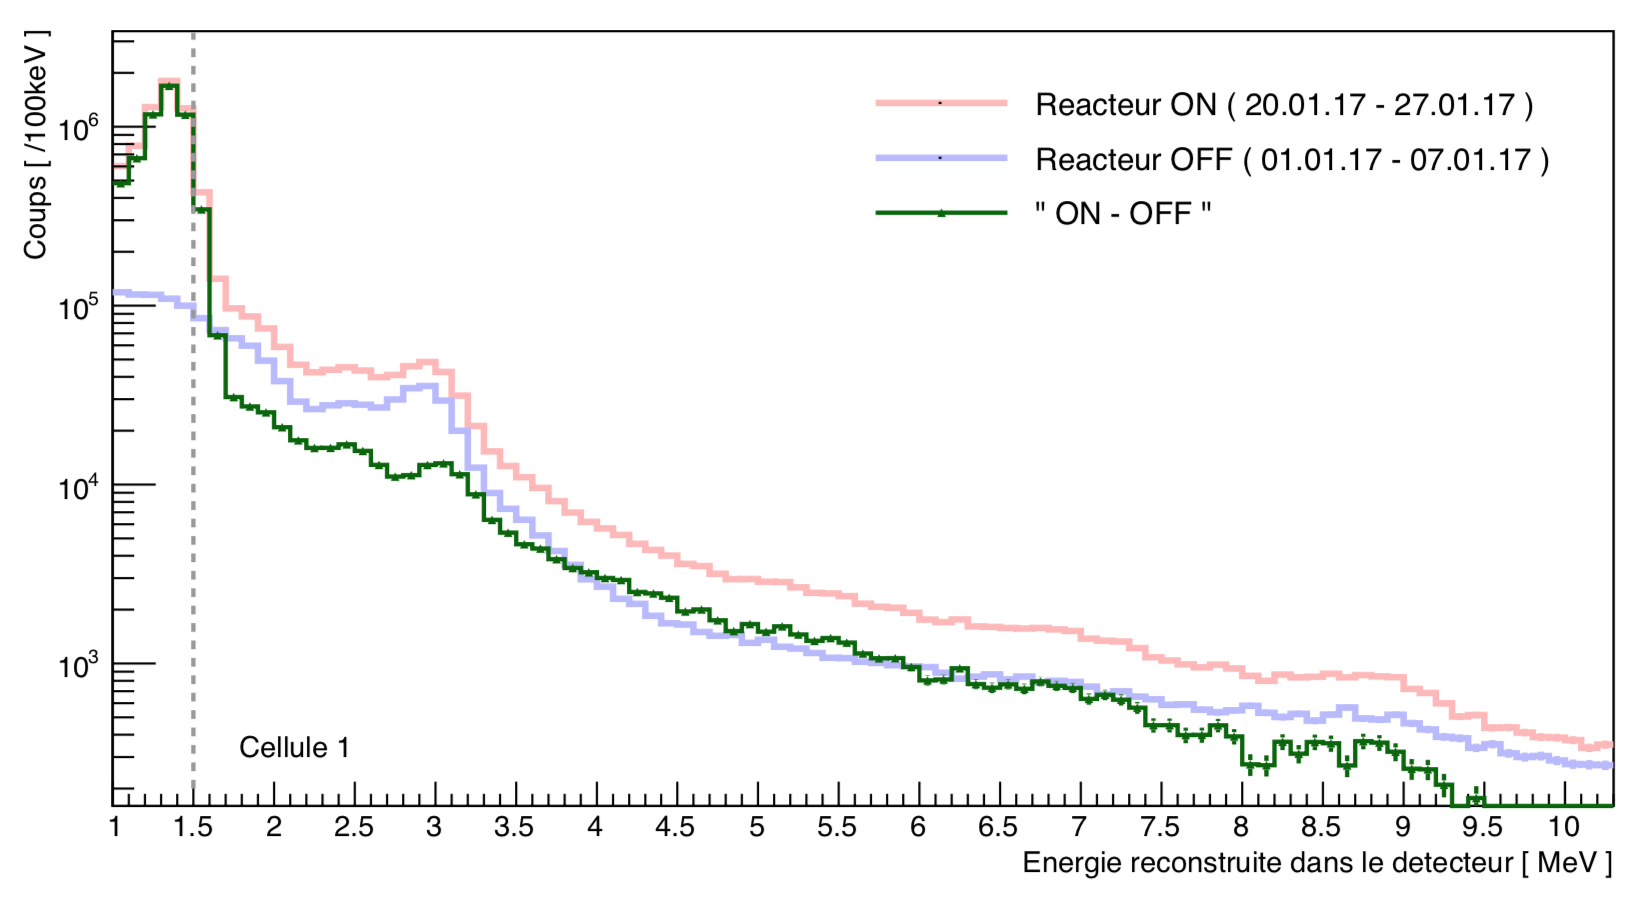
\includegraphics[width=0.9\textwidth]{images/single_spectrum_cell1.png}
\caption[Distribution énergétique des événements simples dans la cellule 1]{Distribution énergétique des événements simples dans la cellule 1. Le spectre en bleu représente les candidats simples dans le détecteur lorsque le réacteur est OFF, tandis que le spectre rouge est le même spectre pendant une période réacteur ON. La distribution en vert correspond à la soustraction "ON - OFF". La ligne verticale en pointillés représente le seuil en énergie pour les candidats Prompt. Le pic en dessous de $\SI{1.5}{MeV}$ correspond en fait à la décroissance du noyau d'$\ce{^{41}Ar}$ dans l'air de l'enceinte du hall expérimental. (source \cite{bonhomme:tel-01931309})}
\label{fig:single_spectrum_cell1.png}

\end{figure}

}


Les bruits de fond simples, très largement majoritaires avant les coupures en temps Prompt-Retardés, s'étalent sur un spectre décroissant de 0 à $\SI{10}{MeV}$ dont les quelques structures qui le composent témoignent de la nature des émetteurs (voire figure \ref{fig:single_spectrum_cell1.png}). Pour éviter d'être submergé par ces bruits de fond à basse énergie, il a été choisi dans l'analyse neutrino de ne garder que les événements qui déposent plus de $\SI{1.5}{MeV}$:

\begin{equation}
    E^\textrm{rec}(\textrm{Prompt}) > \SI{1.5}{MeV}.
\end{equation}

\bigbreak

Afin de limiter la contribution des bruits de fond gamma sur le spectre positron, des contraintes supplémentaires sur l'énergie reconstruite dans les cellules voisines sont imposées:

\begin{align}
\label{eq:neighbor_E_cuts}
    E^\textrm{rec}_{c = (\mathcal{C} \pm 1 \textrm{ ou } c = \{8,9\})} < \SI{1}{MeV},\\
    E^\textrm{rec}_{c \neq (\mathcal{C} \pm 1 \textrm{ ou } c = \{8,9\})} < \SI{400}{keV},
\end{align}

\bigbreak

où les cellules 8 et 9 désignent les longues cellules du Gamma Catcher.

\bigbreak

La signature du neutron attendu dans la fenêtre Retardée se caractérise par la cascade de rayons gammas émis par un noyau de gadolinium. Environ $\SI{8}{MeV}$ sont libérés par cascade et chaque gamma a en moyenne une énergie de $\SI{2}{MeV}$. La distribution spatiale des dépôts d'énergie est plus large, c'est pourquoi le spectre en énergie possède une large queue à basse énergie (voir figure \ref{fig:Data_z45cm-Delay-Diff-Energy.pdf}). Les bornes en énergie sur la fenêtre Retardée ont été choisies pour que la contribution des bruits de fond accidentels soit minime:

\begin{equation}
    \SI{4.5}{MeV} < E^\textrm{rec}(\textrm{Retardé}) < \SI{10}{MeV}.
\end{equation}

\bigbreak

\afterpage{
%Data_z45cm-Delay-Diff-Energy.pdf

\begin{figure}[h!]
\centering
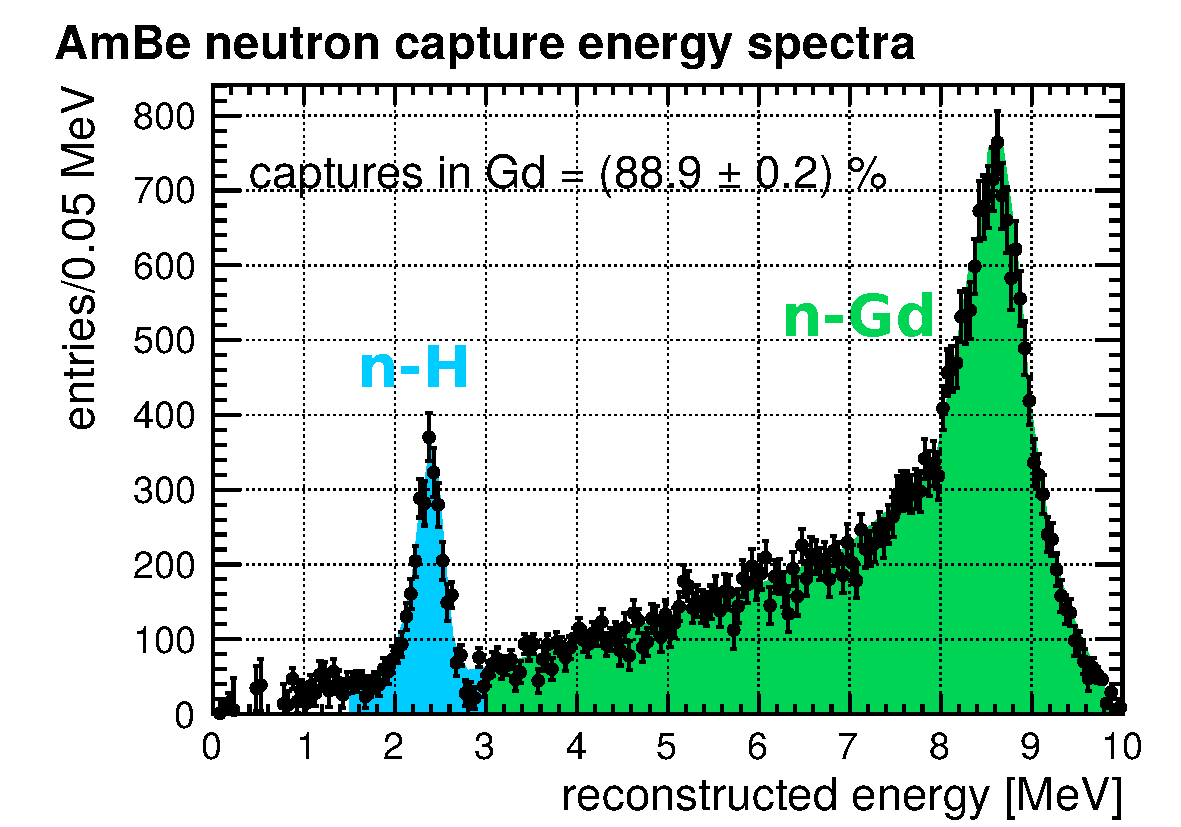
\includegraphics[width=0.9\textwidth]{images/Data_z45cm-Delay-Diff-Energy.pdf}
\caption[Spectre des gammas de capture neutron dans \textsc{Stereo}]{Spectre des gammas de captures neutrons produits par la source d'$\ce{AmBe}$ \cite{docdb548}. Les zones en bleu et en vert représentent respectivement les quantités $N_\textrm{H}$ et $N_\textrm{Gd}$ qui servent à l'ajustement de la concentration de gadolinium dans la simulation.}
\label{fig:Data_z45cm-Delay-Diff-Energy.pdf}

\end{figure}

}

La limite basse basse à $\SI{4.5}{MeV}$ coupe une part non négligeable des captures neutrons. En plus de diminuer l'efficacité de détection neutrino, cette contrainte impose une bonne modélisation de la cascade n-Gd pour minimiser les incertitudes systématiques sur la prédiction du nombre de neutrinos détectés.\\

La présence de gadolinium dans la Target exclusivement nous permet d'appliquer une contrainte supplémentaire sur l'énergie reconstruite :

\begin{equation}
    E^\textrm{rec}_\textrm{Target}(\textrm{Retardé}) > \SI{1}{MeV}.
\end{equation}

\bigbreak

Pareillement à la seconde coupure des événements Prompt, cette contrainte permet de retirer une grande partie des contributions des bruits de fond accidentels à haute énergie.

\bigbreak

Puisque le positron et le neutron issus d'une décroissance Beta inverse sont émis au même endroit, il existe une corrélation spatiale de la lumière produite entre les deux événements. En effet, le positron ne parcourt que quelques centimètres avant d'être annihilé en deux gammas de $\SI{511}{keV}$, qui eux aussi ne déposent de l'énergie que sur quelques centimètres. D'autre part, la diffusion du neutron peut être considérée comme une marche aléatoire où l'information sur la direction d'origine est perdue. Ainsi, à partir d'un grand nombre de collisions $n$, la distance moyenne au point de départ $r$ peut être exprimée par la densité de probabilité \cite{doi:10.1080/14786449908621276}:

\begin{equation}
    P(r) \propto \frac{2}{n} e^{-r^2/n}.
\end{equation}

Autrement dit, et pour citer Karl Pearson : \og \textit{In an open country, the most probable place to find a drunken man, who is at all capable of keeping on his feet, is somewhere near his starting point!} \fg{} \cite{PEARSON:1905fu}. En revanche la variance sur $r$ augmente avec le nombre de chocs, et sur une fenêtre de quelques dizaines de microsecondes sa valeur ne dépasse pas $\SI{20}{cm}$.\\

\bigbreak

La précision sur la reconstruction de la position moyenne des dépôts d'énergie est limitée, car les parois réfléchissantes ont justement été conçues pour homogénéiser la collection de lumière. Néanmoins, la segmentation du volume cible permet d'estimer la position des vertex à $\pm \SI{15}{cm}$ dans le sens de la longueur du détecteur (axe $x$). Pour ce faire, un barycentre sur l'axe $x$ est attribué à chaque événement:

\begin{equation}
    B_x = \frac{\sum_{c = 0}^{10} E^\textrm{rec}_c \times b_c}{\sum_{c = 0}^{10} b_c},
\end{equation}

\bigbreak

où $b_c$ est la position du barycentre en charges collectées par les photomultiplicateurs de la cellule $c$. Ainsi, l'écart entre les barycentres de l'événement Prompt et Retardé est contraint pour réduire les coïncidences fortuites:

\begin{equation}
    | B_x(\textrm{Retardé}) - B_x(\textrm{Prompt})| < \SI{600}{mm} \simeq 1.5 \times \textrm{largeur de cellule}.
\end{equation}

\bigbreak

Étant donné qu'au sein de chaque cellule les photons sont brassés par les parois réfléchissantes, la lumière est collectée de façon relativement équitable entre les photomultiplicateurs. L'asymétrie de collection de charges dans une cellule est définie comme le rapport entre le nombre de photons collectés par le PM qui a reçu le plus de photo-électrons et la charge totale collectée par la somme de tous les PMs de la cellule. L'asymétrie qui est considérée dans l'analyse concerne la cellule qui a reconstruit le plus d'énergie, elle est définie comme suit:

\begin{equation}
    \zeta \doteq \frac{Q_{\textrm{PM(i)}}^\textrm{Max}}{Q_i} \textrm{ avec } i \textrm{ tel que } E_i \geq E_j \forall j \in \left\{ 0, 10\right\}.
\end{equation}

\bigbreak

Bien que la coupure à $\SI{8}{MeV}$ sur l'énergie reconstruite du candidat Prompt élimine la plupart des signaux muons ($dE/dx \geq \SI{2}{MeV/cm}$), une partie d'entre eux persistent et ont une signature qui imite celle des neutrinos: il s'agit des muons qui s'arrêtent en haut d'une cellule et décroissent (\og \textit{muons stop} \fg{}). En effet, ces muons déposent suffisamment d'énergie en haut du détecteur pour passer la coupure Prompt et l'électron produit par leur décroissance (dit \og \textit{électron Michel} \fg{} \cite{Michel:1949qe}) peut être confondu avec une cascade neutron dans la fenêtre Retardée. Ces décroissances ont forcément lieu proche de la surface du liquide scintillateur, au niveau des \textit{buffers}, et par conséquent très proche d'un photomultiplicateur. Leur asymétrie $\zeta$ est anormalement haute, alors la coupure suivante a été choisie :

\begin{equation}
    \zeta < 0.5.
\end{equation}

Les études sur l'efficacité de détection ont montré que cette contrainte permet de rejeter environ 50 \% des \textit{muons stop} tout en conservant 99 \% des neutrinos. Ce critère est appliqué dans les deux fenêtres Prompt et Retardée.

\bigbreak

%\begin{itemize}
%    \item coupures énergie prompt / delay
%    \item veto / GC
%    \item correlation spaciale
%    \item tableau récapitulatif
%    \item Acceptance globale
%\end{itemize}

\subsection{Coupures en temps}
\label{sec:time_cuts_pair_search}

La corrélation temporelle entre la détection du positron et celle du neutron est définie par l'écart entre leurs temps d'occurrence :

\begin{equation}
    \Delta T = T(\textrm{Retardé}) - T(\textrm{Prompt}),
\end{equation}

\bigbreak

où $T(\textrm{Prompt})$ et $T(\textrm{Retardé})$ sont les temps mesurés par discrimination à fraction constante (c.f. section \ref{sec:stereo_elec}). Le temps de capture d'un neutron dans le liquide est le résultat d'une compétition entre la phase de thermalisation et de diffusion. La durée de thermalisation ne dépend que très peu de l'énergie cinétique initiale du neutron, car celle-ci est largement dominée par les dernières collisions: $t_\textrm{inter-collisions} \propto \lambda_n / v_n(t)$ où $\lambda_n$ est la distance moyenne sans collision et $v_n(t)$ la vitesse du neutron qui décroit avec le temps\footnote{Au premier ordre, on peut considérer que la vitesse du neutron diminue de moitié à chaque collision. Le temps entre deux collisions croit alors en puissance de 2 : $t \propto 2^n$, où $n$ est le nombre de chocs subis.}. C'est pourquoi des études sur le temps de capture neutron ont pu être menées avec la source d'AmBe, où les neutrons émis ont une énergie cinétique de l'ordre du MeV contre quelques dizaines de keV pour ceux issus d'une décroissance Beta inverse. Les distributions de temps de capture neutron dans les données et la simulation sont présentés sur la figure \ref{fig:neutron_delta_t_AmBe.pdf}. La section efficace de capture sur un noyau de gadolinium augmente au fur et à mesure que l'énergie du neutron diminue, c'est pourquoi la distribution des $\Delta T$ augmente jusqu'à $\SI{6}{\mu s}$. L'allure décroissante après $\SI{10}{\mu s}$ de la courbe suit une loi exponentielle dont la constante de temps $\tau_\textrm{Gd}$ est caractéristique de la section efficace de capture pour des neutrons thermiques (c.f. Equation (\ref{eq:neutron_capture_time})) : $\SI{16}{\mu s}$.\\

\afterpage{
% neutron_delta_t_AmBe.pdf

\begin{figure}[h!]
\centering
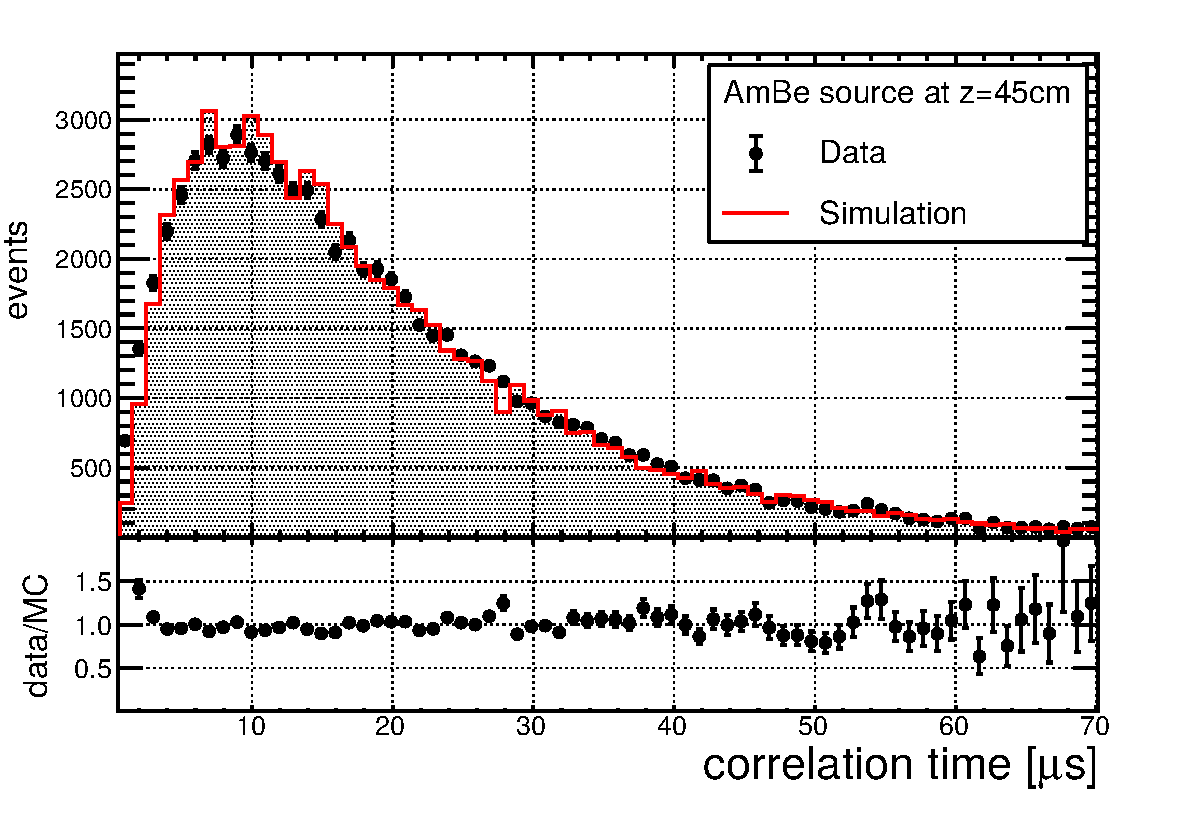
\includegraphics[width=0.8\textwidth]{images/neutron_delta_t_AmBe.pdf}
\caption[Distributions des temps de captures neutrons produits par la source d'$\ce{AmBe}$]{Comparaison données simulation des distributions de temps de captures neutrons produits par la source d'$\ce{AmBe}$ placée au centre d'une cellule. (source : \cite{docdb861})}
\label{fig:neutron_delta_t_AmBe.pdf}

\end{figure}

\begin{figure}[h!]
\centering
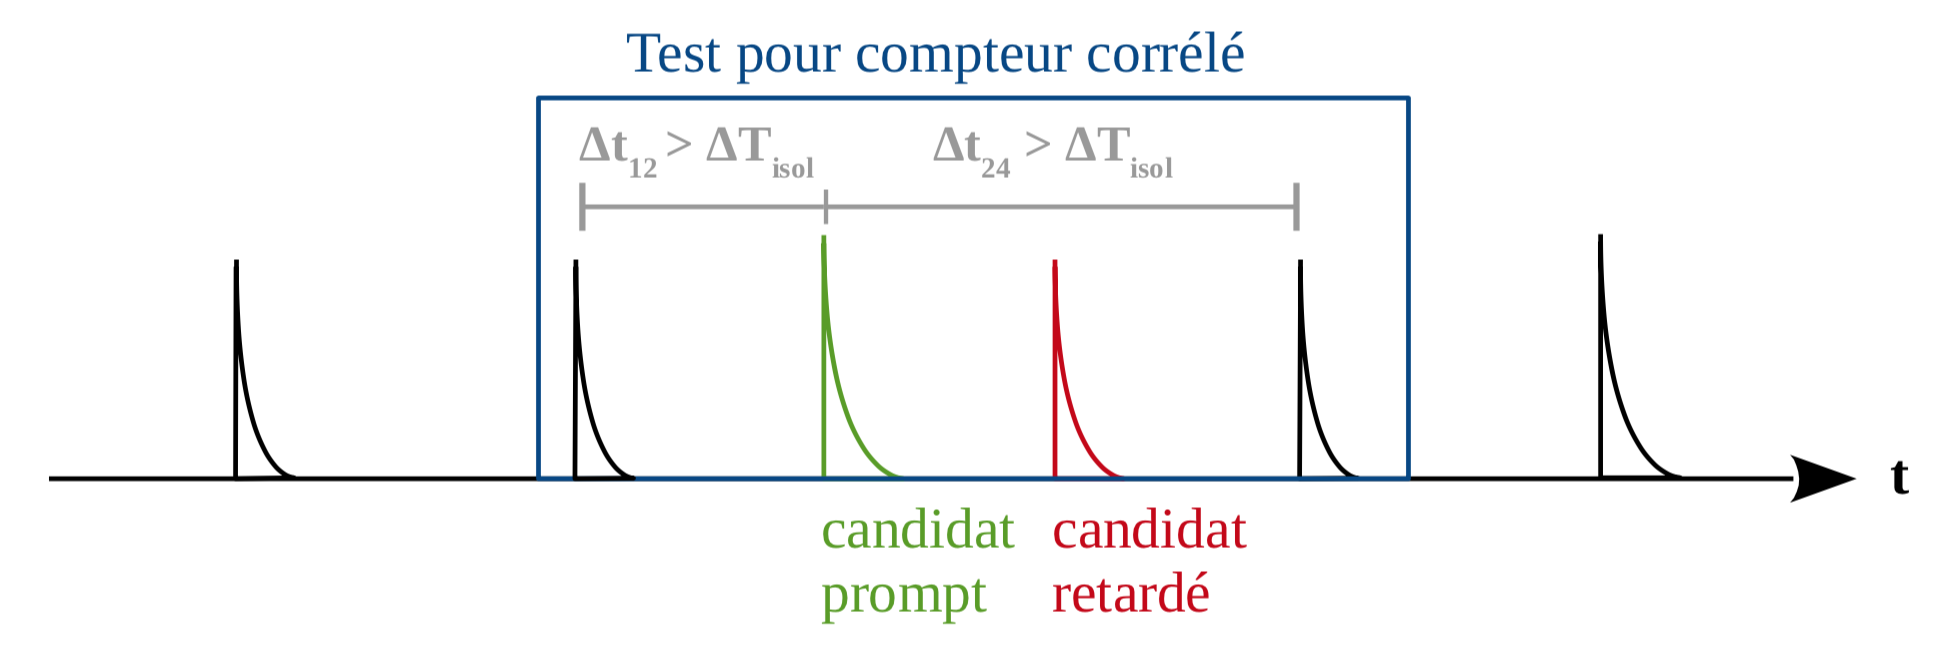
\includegraphics[width=1\textwidth]{images/principe_coupures_isolation_temps.png}
\caption[Principe des coupures temporelles sollicitées pour extraire les événements IBD]{Principe des coupures temporelles sollicitées pour extraire les événements IBD. (source : \cite{bonhomme:tel-01931309})}
\label{fig:principe_coupures_isolation_temps.png}

\end{figure}

}

La coupure haute sur $\Delta T$ a été choisie à $\SI{70}{\mu s}$ pour maximiser l'acceptance des signaux neutrino ($\sim \SI{98}{\%}$) tout en réduisant la contribution des bruits de fond. Aussi, un seuil en temps a été fixé à $\SI{2}{\mu s}$ pour éliminer le reste des événements \textit{muons stop} qui ont survécu la coupure sur l'asymétrie $\zeta$, au prix d'environ $\SI{2}{\%}$ d'efficacité de détection. Les bornes retenues pour l'analyse neutrino sont :

\begin{equation}
\label{eq:delta_T_prompt_delayed}
    \SI{2}{\mu s} < T(\textrm{Retardé}) - T(\textrm{Prompt}) \doteq \Delta T < \SI{70}{\mu s}.
\end{equation}

\bigbreak

Par ailleurs, des critères d'isolation temporelle de la paire candidate ont été ajoutés pour rejeter davantage les paires d'événements dont l'origine est cosmique. En effet, l'interaction des muons à proximité du détecteur peut engendrer de multiples particules susceptibles de déposer de l'énergie dans le liquide. De par leur nature, ces bruits de fond sont corrélés et passent donc aisément la coupure en $\Delta T$. Leurs critères de réjection sont basés sur l'identification des muons cosmogéniques.\\

Le véto muon qui surplombe le détecteur étiquette le passage d'un muon dans l'eau par effet Cherenkov. Il a été montré que l'efficacité de détection des muons était supérieure à $\SI{99}{\%}$ \cite{docdb445}. Cependant lorsque leur angle d'incidence est trop important, certains muons atteignent le volume cible et déposent de l'énergie dans le liquide scintillateur sans passer par le véto. Au minimum d'ionisation, les muons déposent environ $\SI{2}{MeV/cm}$ et donc après moins de $\SI{10}{cm}$ dans le liquide, $\SI{20}{MeV}$ ont été déposés. Au-dessus de cette énergie peu d'autres bruits de fond sont présents, par conséquent il a été choisi d'étiqueter arbitrairement comme muon tout événement dont l'énergie reconstruite est supérieure à $\SI{20}{MeV}$. La fréquence de muons étiquetés est d'environ $\SI{850}{Hz}$, dont $\SI{650}{Hz}$ sont détectés dans le véto et $\SI{400}{Hz}$ dans le détecteur avec 20 \% d'overlap. À chaque muon est attribué le temps d'arrivée $t_\mu$ et, dans le cadre de la recherche de paires corrélées en temps, le temps d'arrivée du dernier muon est défini comme:

\begin{equation}
    T_\mu \doteq \underset{t_\mu}{\operatorname{argmax}} \left( t_\mu | t_\mu < T(\textrm{Signal})\right),
\end{equation}

\bigbreak

où $T(\textrm{Signal})$ est la date de déclenchement de l'acquisition pour n'importe quel signal: Prompt, Retardé, ou Simple. Pour limiter la contribution des bruits de fond d'origine cosmique, chaque événement doit satisfaire la condition suivante :

\begin{equation}
\label{eq:cut_muon_veto}
    \Delta T_\mu \doteq T(\textrm{Signal}) - T_\mu > \SI{100}{\mu s}.
\end{equation}

\bigbreak

Notons que cette condition implique un \og \textit{temps mort} \fg{} d'acquisition de l'ordre de $R_\mu \Delta T_\mu$, où $R_\mu$ est la fréquence moyenne d'étiquetage muon. L'estimation du temps mort est calculée précisément à chaque run avec l'algorithme de recherche de paire décrit dans la section suivante.\\

\afterpage{

\begin{table}
  \begin{center}
    \begin{tabular}{|c|c|c|}
    \hline
      Type & Étiquette & Critère de sélection\\
      \hline
      \hline
      \multirow{6}{*}{Prompt} & A & $\SI{1.5}{MeV} < E^\textrm{rec}(\textrm{Prompt}) < \SI{8}{MeV}$\\
      & B & $E^\textrm{rec}_\textrm{GC}(\textrm{Prompt}) < \SI{1.1}{MeV}$\\
      & C & $\mathcal{C} \doteq c \textrm{ tel que } E_c^\textrm{rec} > E_{c'}^\textrm{rec} \forall c' \neq c$\\
      & D & $E^\textrm{rec}_{c = (\mathcal{C} \pm 1 \textrm{ ou } c = \{8,9\})} < \SI{1}{MeV}$\\
      & E & $ E^\textrm{rec}_{c \neq (\mathcal{C} \pm 1 \textrm{ ou } c = \{8,9\})} < \SI{400}{keV}$\\
      & F & $\zeta < 0.5$\\
      \hline
      \multirow{3}{*}{Retardé} & G & $\SI{4.5}{MeV} < E^\textrm{rec}(\textrm{Retardé}) < \SI{10}{MeV}$\\
      & H &  $E^\textrm{rec}_\textrm{Target}(\textrm{Retardé}) > \SI{1}{MeV}$\\
      & I & $\zeta < 0.5$\\
      \hline
      Corrélation spatiale & J & $| B_x(\textrm{Retardé}) - B_x(\textrm{Prompt})| < \SI{600}{mm}$\\
      \hline
      Corrélation temporelle & K & $\SI{2}{\mu s} < \Delta T < \SI{70}{\mu s}$\\
      \hline
      \multirow{2}{*}{Véto Muon} & L & $\Delta T_\mu > \SI{100}{\mu s}$\\
      & M & $Q_\textrm{veto} < \SI{80}{pe}$\\
      \hline
      \multirow{2}{*}{Isolation temporelle} & N & $\Delta T_\textrm{isol}^\textrm{before} > \SI{100}{\mu s}$\\
      & O & $\Delta T_\textrm{isol}^\textrm{after} > \SI{100}{\mu s}$\\
      \hline
    \end{tabular}
  \end{center}
  \caption{Liste des coupures topologiques et temporelles utilisées pour l'extraction du signal neutrino.}
    \label{tab:neutrino_cuts_base}
\end{table}

}

Il arrive parfois que le muon ne soit pas directement détecté, mais que la gerbe de particules qu'il génère le soit. Ces particules étant corrélées en temps peuvent imiter la signature de la décroissance Beta inverse. Afin de s'affranchir de cette composante de bruit de fond, une coupure d'isolation des paires Prompt-Retardé est imposée:

\begin{equation}
\label{eq:isolation_cut}
    \begin{gathered}
        \Delta T_\textrm{isol}^\textrm{before} \doteq T(\textrm{Prompt}) - T(\textrm{Simple}) > \SI{100}{\mu s} \ \textrm{ et }\\
    \Delta T_\textrm{isol}^\textrm{after} \doteq T(\textrm{Simple}) - T(\textrm{Prompt}) > \SI{100}{\mu s}.
    \end{gathered}
\end{equation}

\bigbreak

Pareillement à la coupure muon, cette condition implique un temps mort estimé par l'algorithme de recherche de paires. La taille des fenêtres d'isolation temporelle a été optimisée en calculant l'évolution de l'erreur statistique du signal neutrino en fonction du temps mort. Le principe des coupures temporelles est résumé par le schéma dessiné sur la figure \ref{fig:principe_coupures_isolation_temps.png}.\\

Finalement, l'ensemble des coupures utilisées dans l'analyse est reporté dans le Tableau \ref{tab:neutrino_cuts_base}. Les lettres correspondantes à chaque coupure interviennent dans les discussions suivantes.

%\begin{itemize}
%    \item delta t plot
%    \item critères d'isolation des paires
%\end{itemize}

\bigbreak

\subsection{Contrôle des biais sur l'efficacité de détection}
\label{sec:neutrino_biases_eff}

\afterpage{

% total_efficiency_proton_spectra.png

\begin{figure}[h!]
\centering
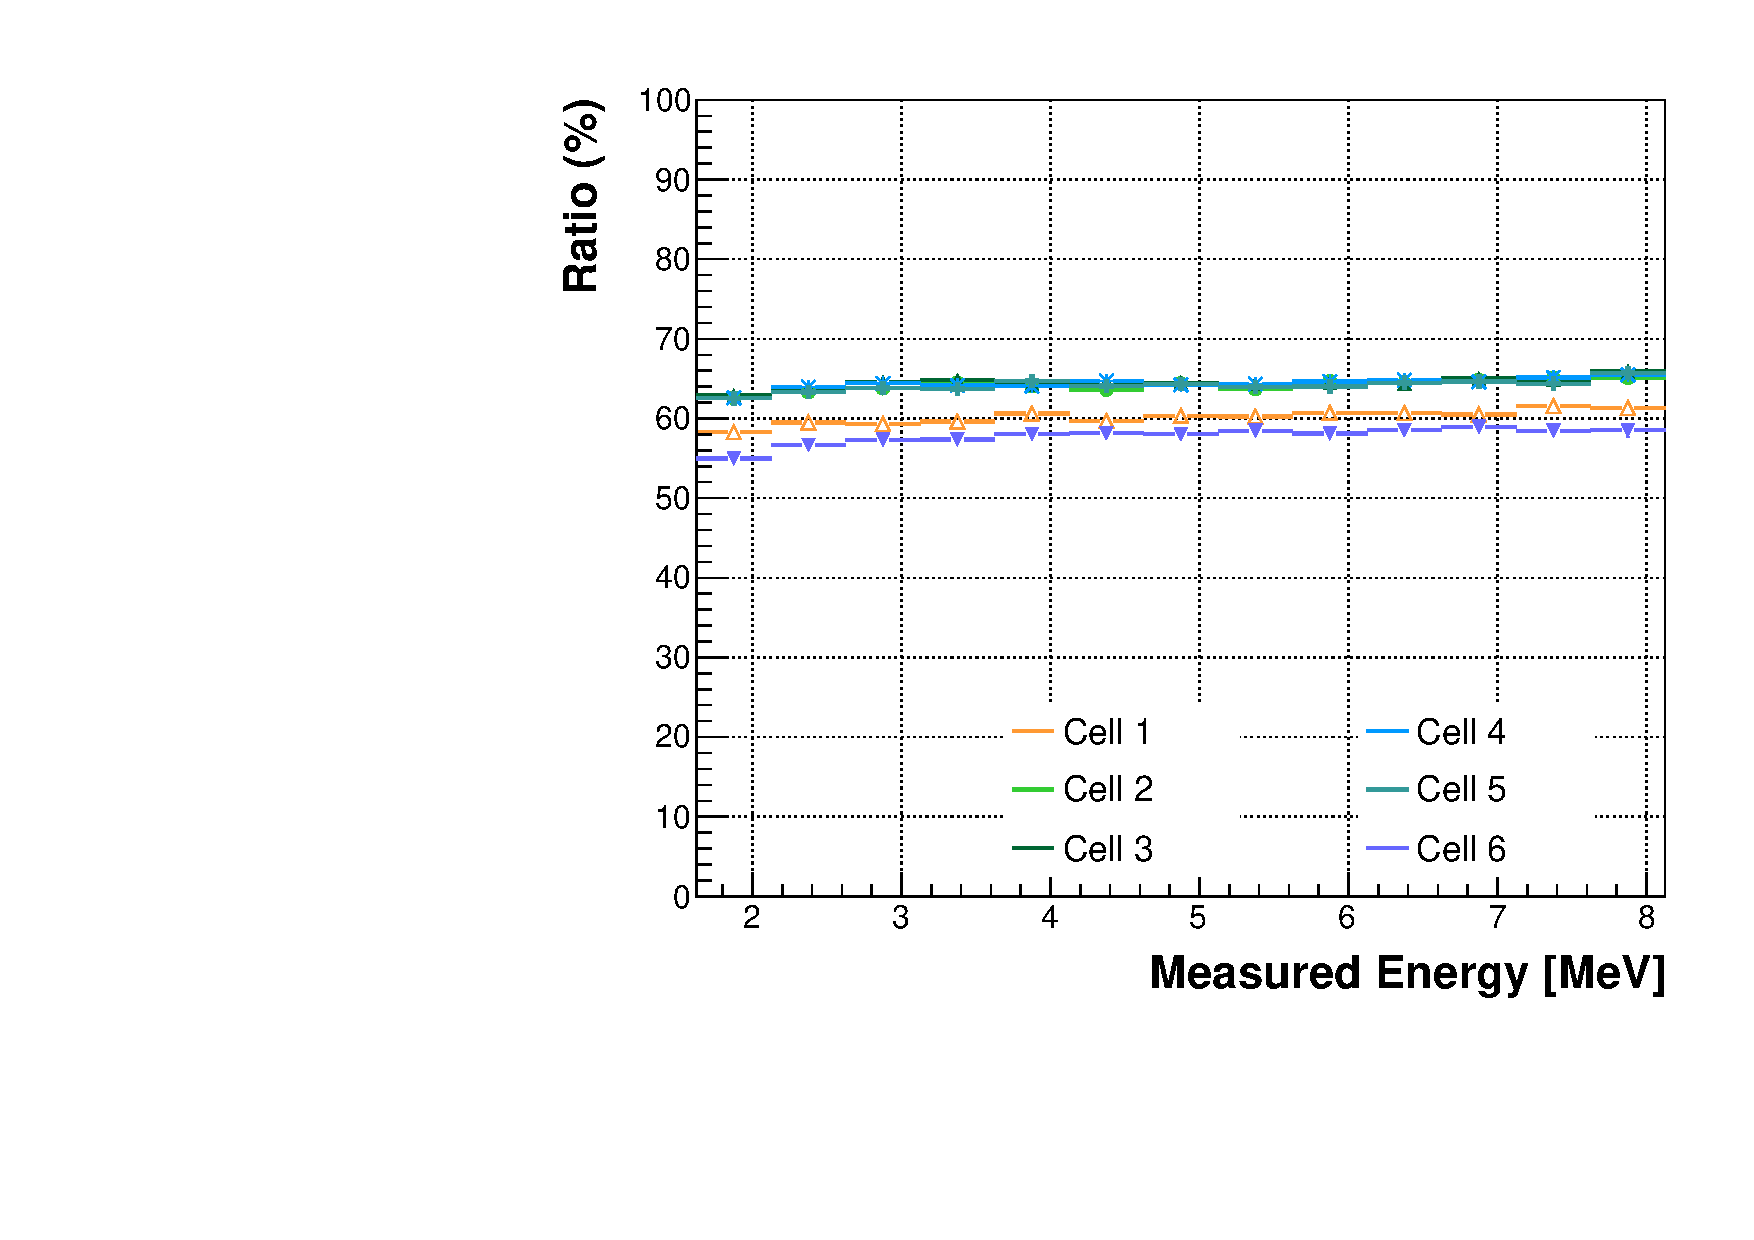
\includegraphics[width=0.7\linewidth]{images/cutAcceptanceByEnergy.pdf}
\caption[Distorsions induites par les coupures topologiques sur le spectre positron]{Distorsions induites par les coupures topologiques sur le spectre positron. (source : \cite{docdb706})}
\label{fig:total_efficiency_proton_spectra.pdf}
\end{figure}

}

À cause de la complexité des effets de volume sur la collection de lumière, l'efficacité des coupures dans la simulation peut légèrement différer de celle  des données. Les désaccords dans la simulation doivent être identifiés pour être corrigés en aval dans l'analyse si besoin. Cette partie est consacrée à l'évaluation de ces biais.\\

\subsubsection*{Efficacité de détection de l'événement Prompt}

%Puisque l'événement Prompt contient l'information sur l'énergie du neutrino incident, la coupure B à $\SI{1.1}{MeV}$ au lieu des $\SI{511}{keV}$ "naturels" a été choisie suffisamment lâche pour éviter toute distorsion du spectre. Cependant, les coupures sur les cellules voisines (\ref{eq:neighbor_E_cuts}) peuvent introduire des biais sur l'acceptance qui dépendent de l'énergie totale. En effet, comme il a été dit dans la Section \ref{seq:Erec_tuning}, un biais sur le coefficient de fuite lumière introduit un décalage sur l'énergie reconstruite dans la cellule voisine :
%
%\begin{equation}
%    \delta E_{2} \propto \delta L_{12} E_1,
%\end{equation}
%
%\bigbreak
%
%avec l'indice $1$ qui représente la cellule où le vertex IBD a été identifié ($\mathcal{C}$) et l'indice $2$ pour une cellule voisine. Puisque le biais $\delta E_{2}$ est proportionnel à l'énergie $E_1$, l'efficacité de la coupure sur $E_{2}$ varie en fonction de l'énergie totale du Prompt. Cet effet est illustré sur la figure \ref{fig:Prompt_Erec_neighbor}. La raison pour laquelle la valeur de $\delta L_{12}$ n'est pas nulle alors que les fuites de lumière ont été ajustées précisément sur le $\ce{^{54}Mn}$, provient du fait que la répartition des dépôts d'énergie pour les neutrinos est homogène contrairement à ceux des gammas du $\ce{^{54}Mn}$ qui sont centrés autour du tube de calibration. Bien que les dépôts d'énergie soient bien décrits par les simulations \textsc{Géant4} et que la procédure de reconstruction ne corrige les effets sur la collection de lumière au premier ordre: les propriétés optiques des parois peuvent différer au second ordre.\\
%
%Cependant, la comparaison des spectres neutrino dans les données avec et sans coupure sur les voisins a montré qu'aucune distorsion significative n'était induite avec une contrainte sur les cellules voisines à $\SI{1}{MeV}$ \cite{docdb695}.\\
%
%\begin{figure}[h!]
%\centering
%\begin{subfigure}[b]{0.49\textwidth}
%
%\centering
%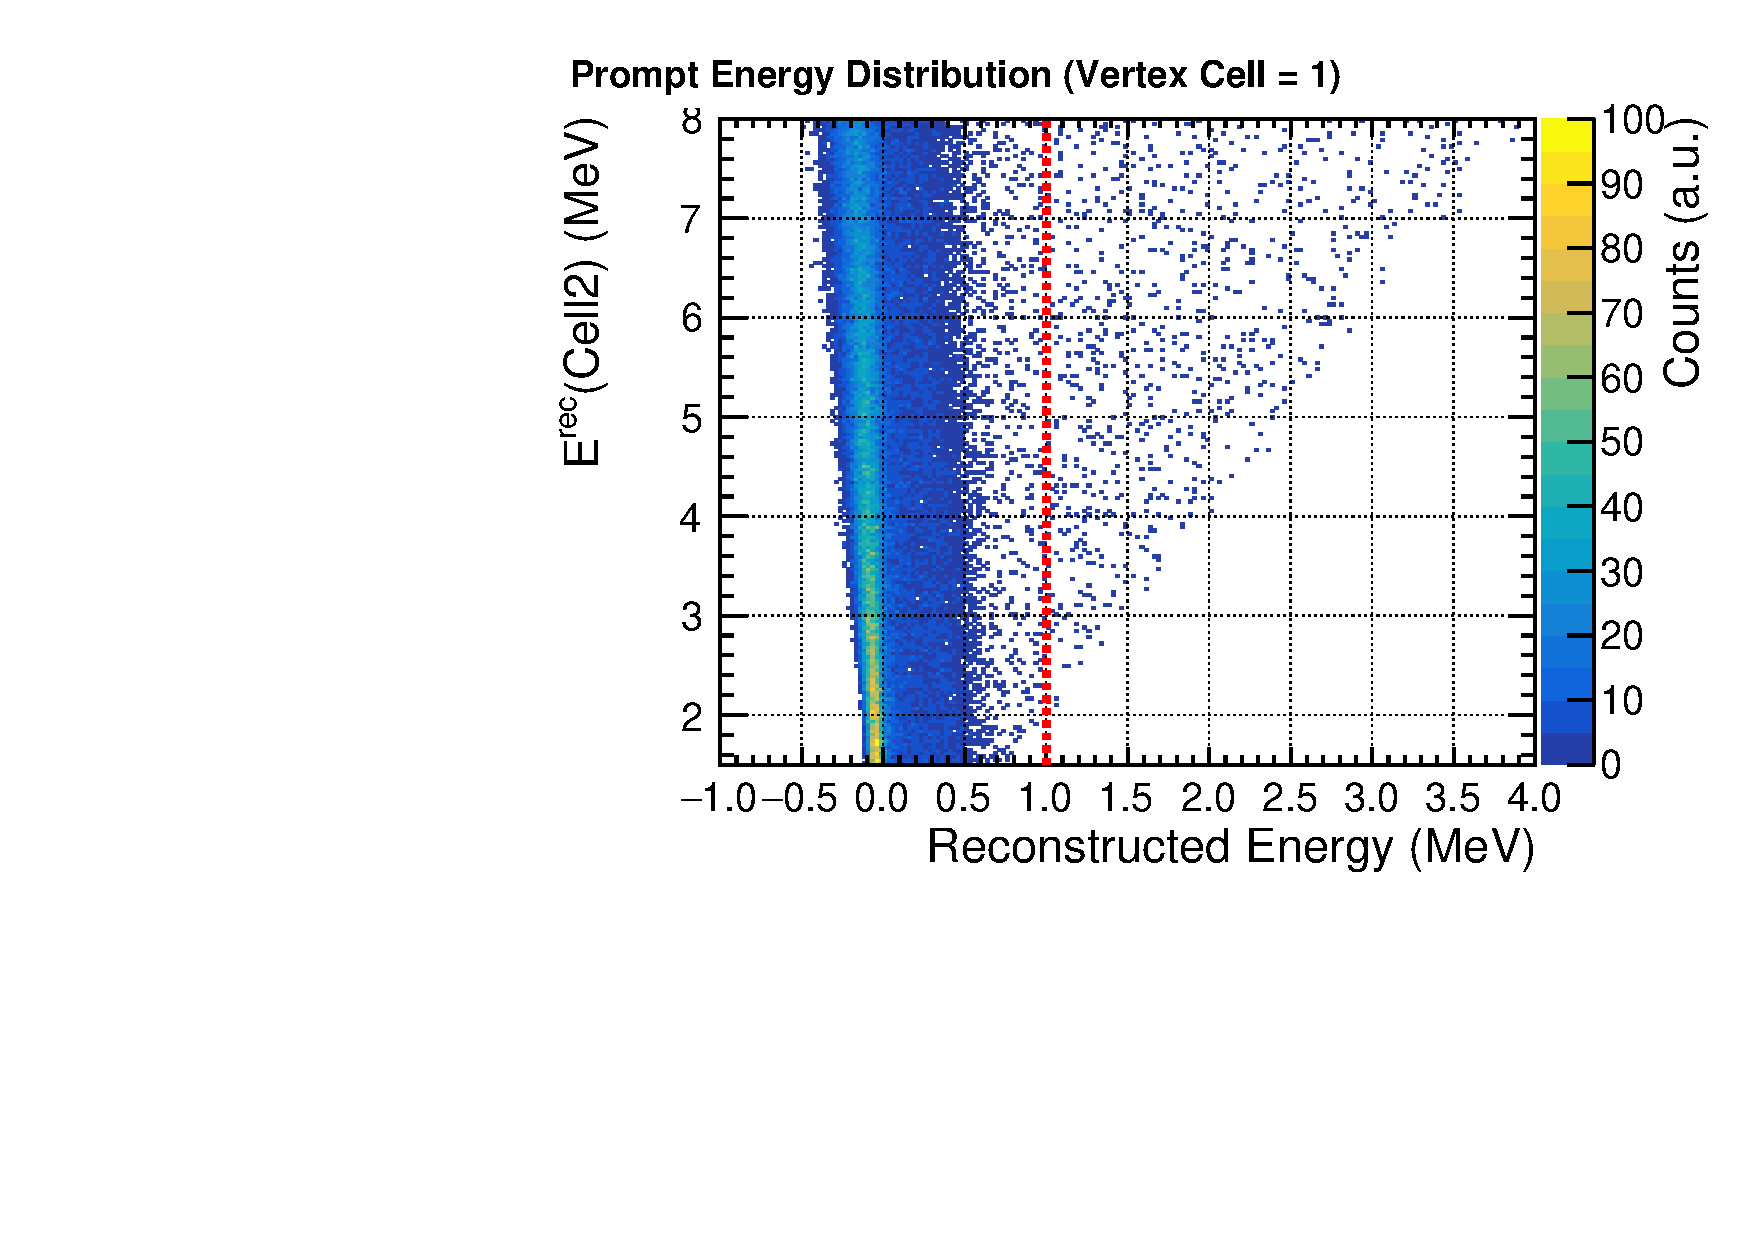
\includegraphics[width=1\linewidth]{images/Prompt_Erec_neighbor_1_to_2.pdf}
%\caption{Vertex localisé dans la cellule 1.}
%\label{fig:Prompt_Erec_neighbor_1_to_2.pdf}
%
%\end{subfigure}
%~ % attention ! space sensitive
%\begin{subfigure}[b]{0.49\textwidth}
%
%\centering
%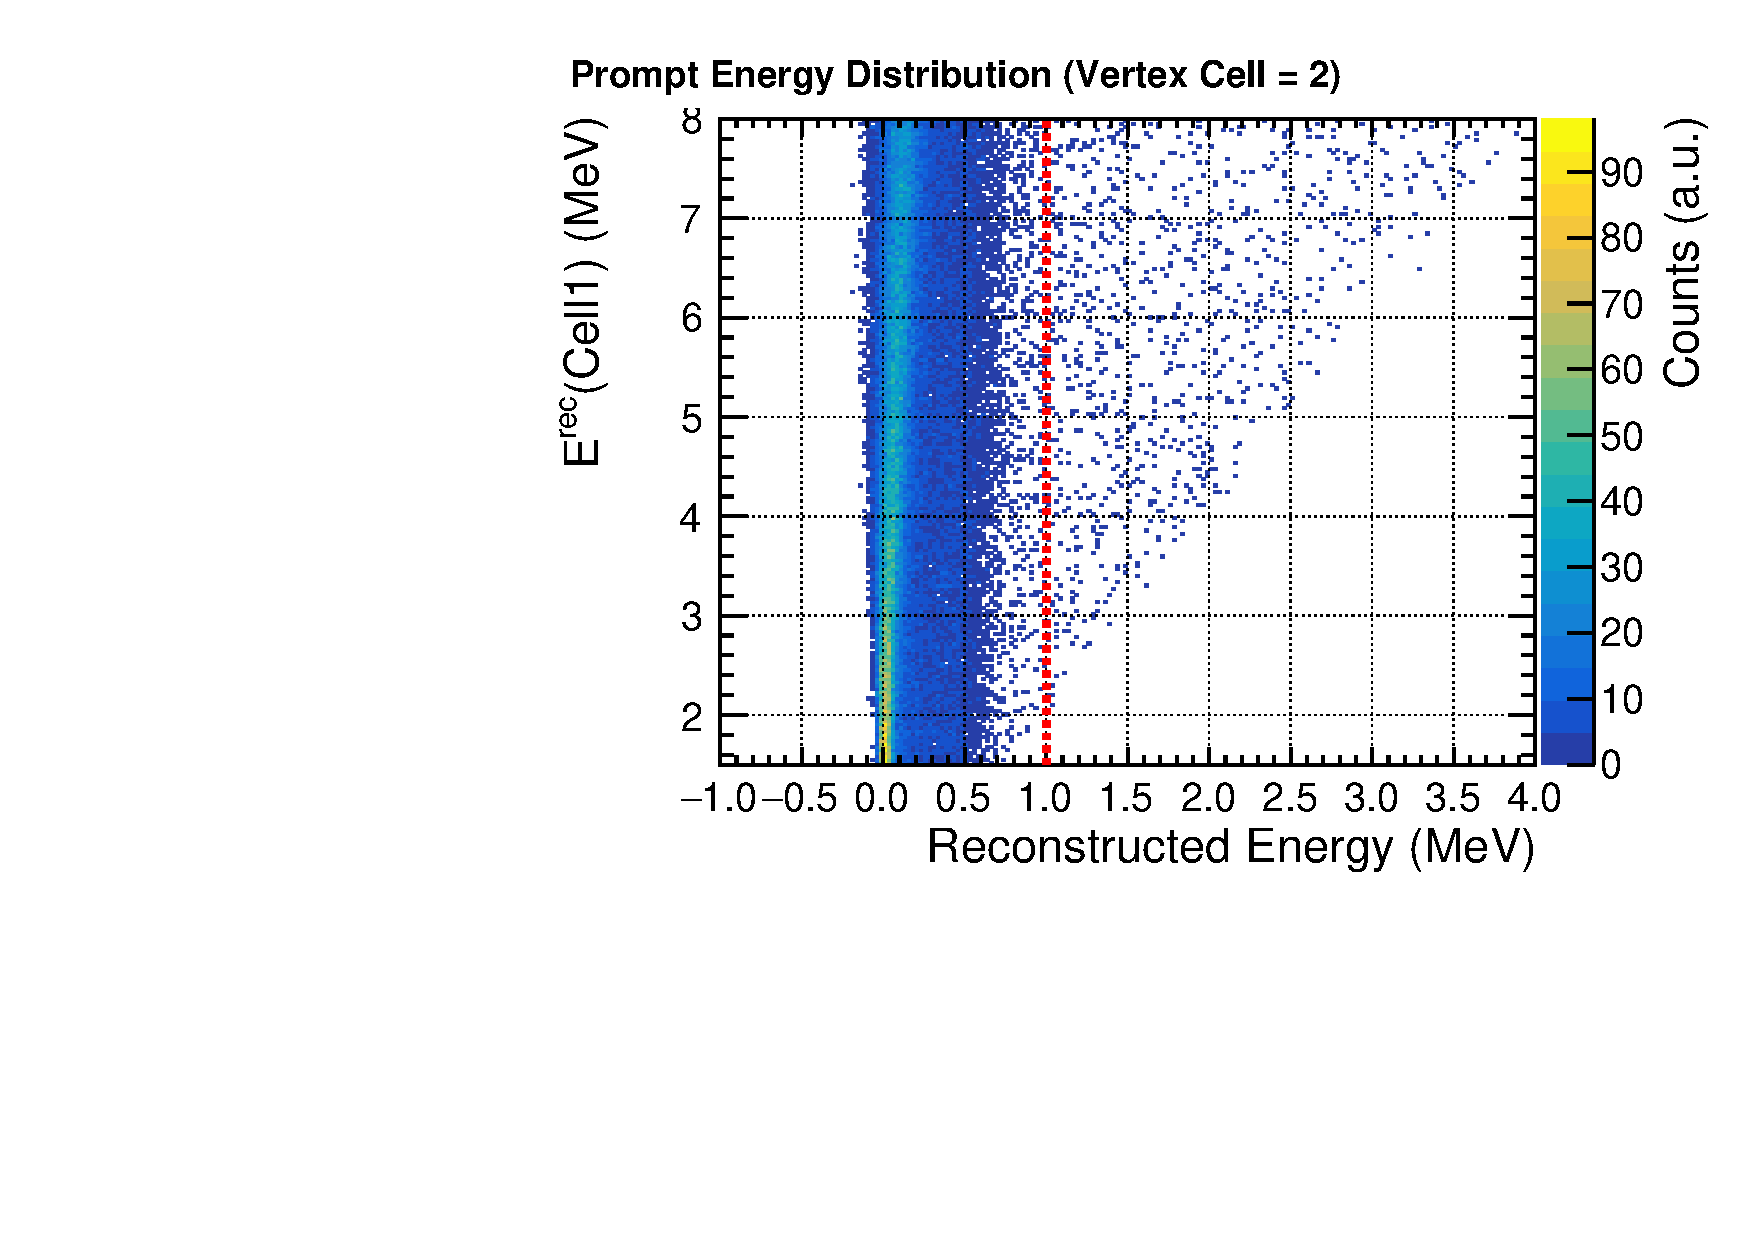
\includegraphics[width=1\linewidth]{images/Prompt_Erec_neighbor_2_to_1.pdf}
%\caption{Vertex localisé dans la cellule 2.}
%\label{fig:Prompt_Erec_neighbor_2_to_1.pdf}
%
%\end{subfigure}
%\caption[Comparaison entre l'énergie du Prompt et l'énergie reconstruite dans une cellule voisine pour des neutrinos simulés.]{Comparaison entre l'énergie du Prompt et l'énergie reconstruite dans une cellule voisine pour des neutrinos simulés. La pente résiduelle est due à un biais sur les coefficients de fuites de lumière utilisés lors de la procédure de reconstruction en énergie. La ligne rouge représente la coupure choisie dans l'analyse.}
%\label{fig:Prompt_Erec_neighbor}
%\end{figure}

L'effet des coupures sur les spectres en énergie des positrons dans chaque cellule a été étudié avec la simulation. Les données MC utilisées sont générées suivant la procédure décrite dans la section \ref{sec:neutrino_simulation}. L'efficacité des coupures est présentée pour chaque cellule par bin en énergie sur la figure \ref{fig:total_efficiency_proton_spectra.pdf}. Les cellules situées au centre du détecteur (2,3,4 et 5) ont une efficacité moyenne de 64 \% avec des distorsions similaires contenues dans une bande de $\pm 2\%$. Cela signifie que dans le scénario sans neutrino stérile, les spectres positrons mesurés doivent avoir la même forme. Les cellules 1 et 6 en revanche sont situées près des bords et montre une efficacité plus faible : 60 \% pour la cellule 1 et 58 \% pour la 6. Cette chute d'efficacité est en fait essentiellement causée par la contrainte sur l'énergie reconstruite dans la Target de l'événement Retardé (H). En effet, puisque la cascade du gadolinium produit plusieurs gammas isotropiquement dans le détecteur, certains peuvent traverser la Target sans y déposer de l'énergie et finalement s'arrêter dans le Gamma-Catcher. La probabilité qu'un tel cas de figure se produise est accrue en bordure de la Target. Pour terminer, le fait que la cellule 1 a une meilleure efficacité que la 6 provient de l'impulsion initiale attribuée au neutron lors de la simulation d'une IBD. Lorsqu'un neutrino interagit avec un proton, le neutron fils est généré avec une impulsion de quelques dizaines keV dans la direction de propagation du neutrino, tandis que le positron est émis plutôt vers l'arrière\footnote{Le positron est émis légèrement vers l'arrière pour des énergies entre 0 et $\SI{10}{MeV}$ : $<\textrm{cos}(\theta)> \simeq -0.02$ où $\theta$ est l'angle entre la direction du neutrino et celle du positron. \cite{Vogel:1999zy}}. Les neutrons créés près de la bordure qui sépare la cellule 1 du Gamma-Catcher Front sont donc ramenés vers l'intérieur de la cible tandis qu'ils sont repoussés vers l'extérieur dans le cas de la 6. Les gammas en cascade émis depuis la limite de la cellule 6 ont donc une probabilité plus forte de déposer moins de $\SI{1}{MeV}$ dans la Target.

\bigbreak

\subsubsection*{Fraction de captures neutrons sur gadolinium}

Une autre source de biais dans l'efficacité de détection concerne la coupure en énergie sur l'événement Retardé. Puisque ce signal est lavé de toute information sur le neutrino incident, il est possible de comparer l'efficacité de détection entre les données et la simulation à l'aide de la source neutron : AmBe. Le noyau d'Américium 241 est un émetteur $\alpha$ avec une durée de vie de 433 ans. Une faible fraction des particule $\alpha$ émises dans le composé se fait capturer par le noyau de Béryllium 9 pour former un Carbone 13 excité qui libère un neutron. Le noyau de Carbone se désexcite en émettant un gamma de $\SI{4.438}{MeV}$ dans 75 \% des cas. L'algorithme de cherche de paires corrélées en temps (décrit dans la section suivante) est exploité pour isoler les signaux de captures des neutrons quelques microsecondes (entre 0 et 100) après la détection du gamma de $\SI{4.438}{MeV}$. Le spectre des gammas de capture est finalement comparé avec la simulation.\\

% 𝑇_1/2 = ℏln2/Γ
% 6,582 119 514(40) × 10−16

\afterpage{

%FIFRELIN_vs_GLG4Sim_new.pdf
\begin{figure}[h!]
\centering
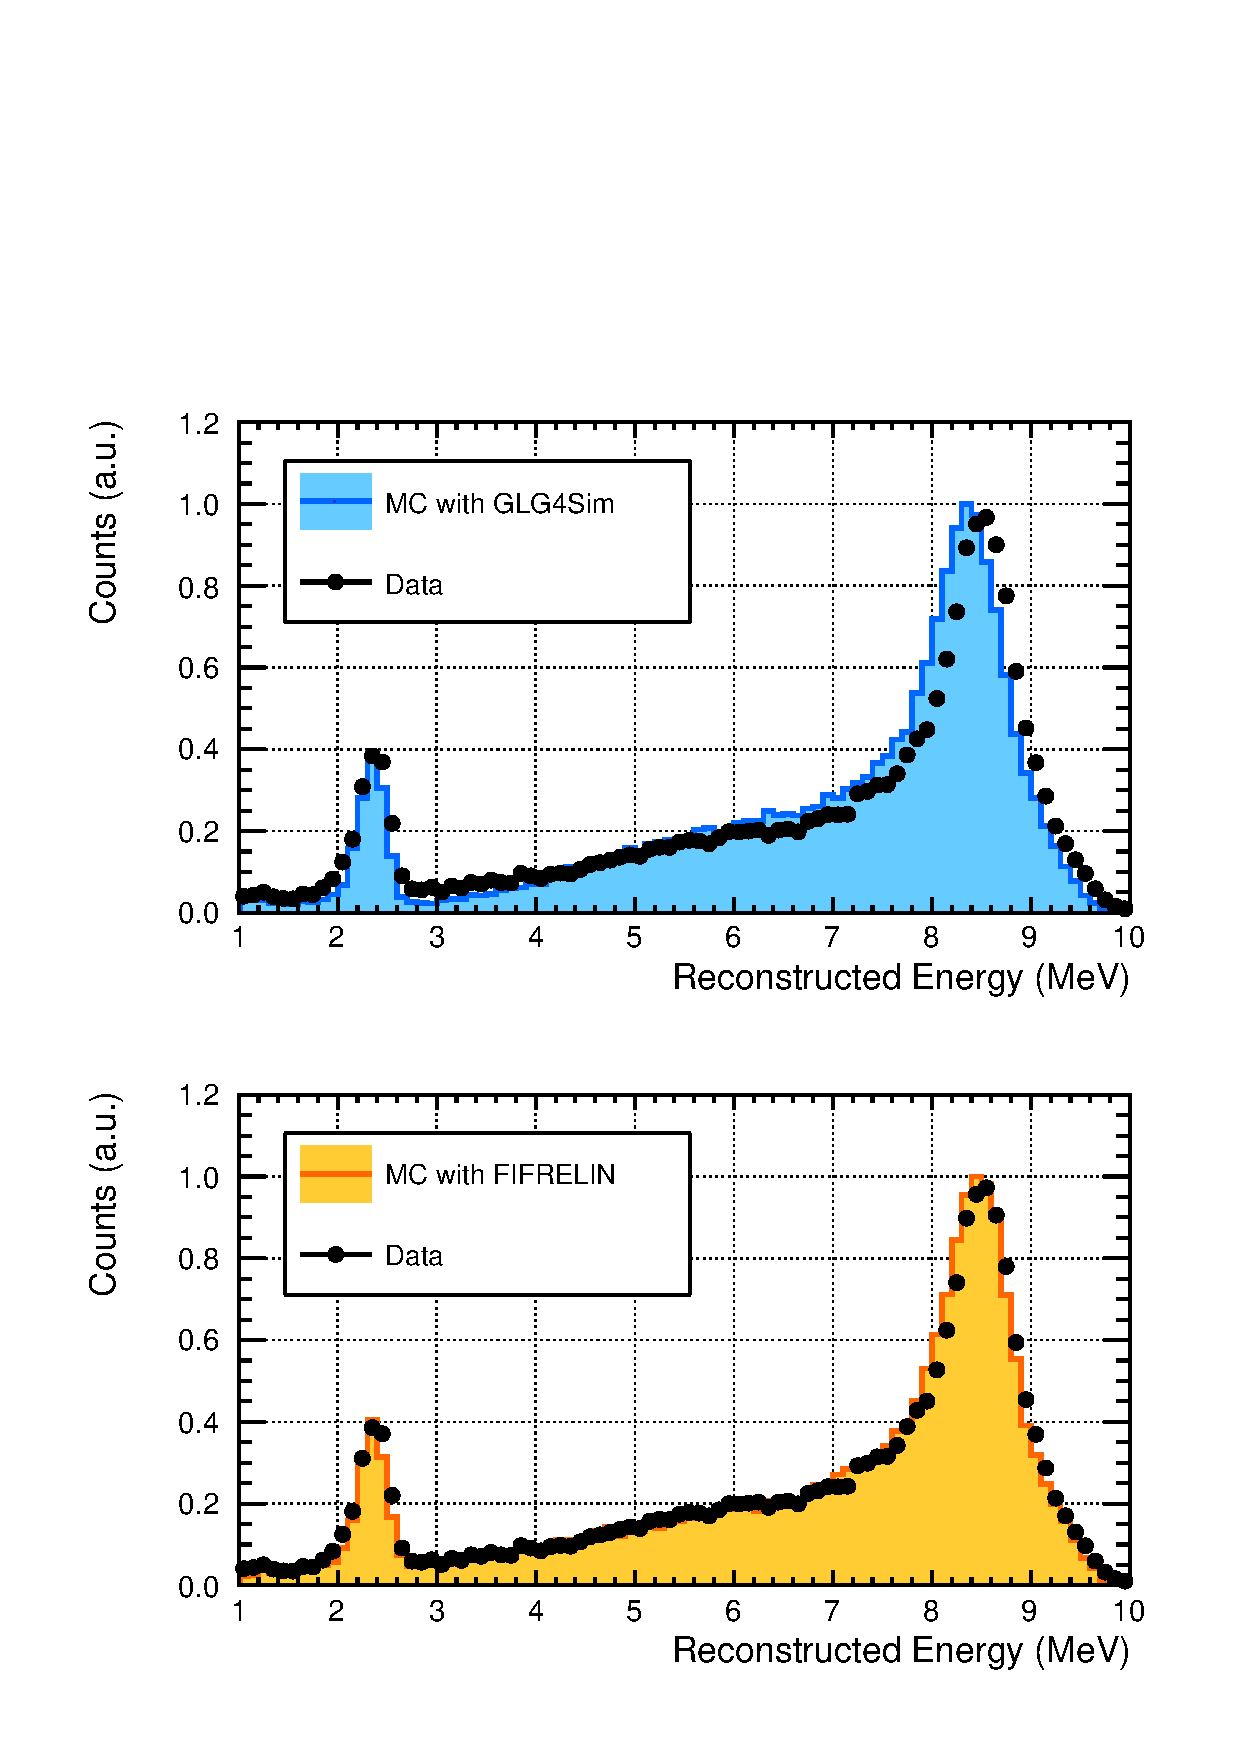
\includegraphics[width=0.7\linewidth]{images/FIFRELIN_vs_GLG4Sim_new.pdf}
\caption[Mise à l'épreuve des simulations des cascades gammas FIFRELIN et GLG4Sim avec les données]{Mise à l'épreuve des simulations des cascades gammas FIFRELIN et GLG4Sim avec les données.}
\label{fig:FIFRELIN_vs_GLG4Sim_new.pdf}
\end{figure}

%C_Gd_fraction.png

\begin{figure}[h!]
\centering
\begin{subfigure}[b]{0.49\textwidth}

\centering
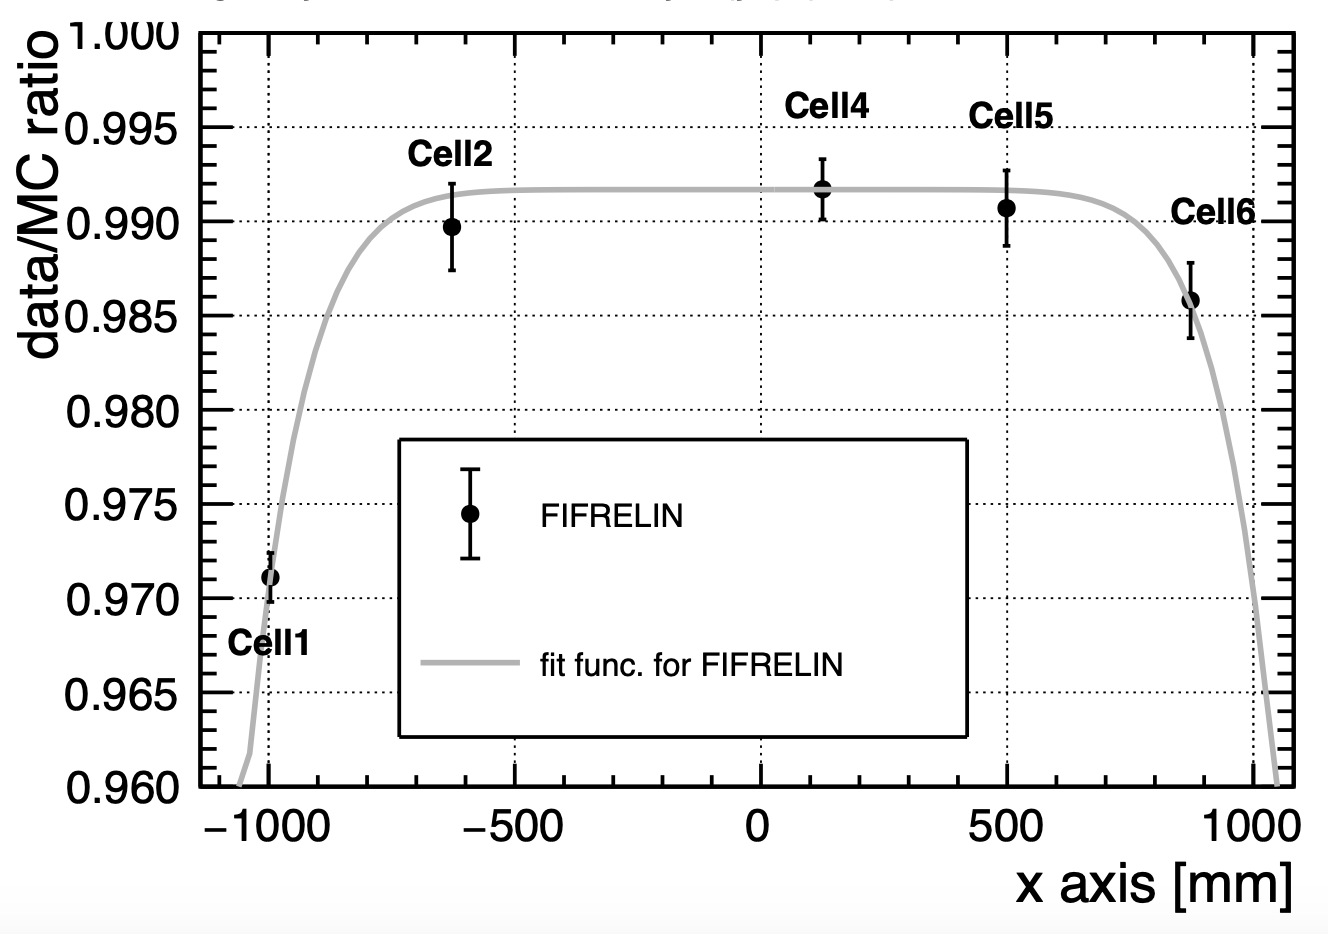
\includegraphics[width=1\linewidth]{images/f_x_Gd_fraction.png}
\caption{}
\label{fig:f_x_Gd_fraction.png}

\end{subfigure}
~ % attention ! space sensitive
\begin{subfigure}[b]{0.49\textwidth}

\centering
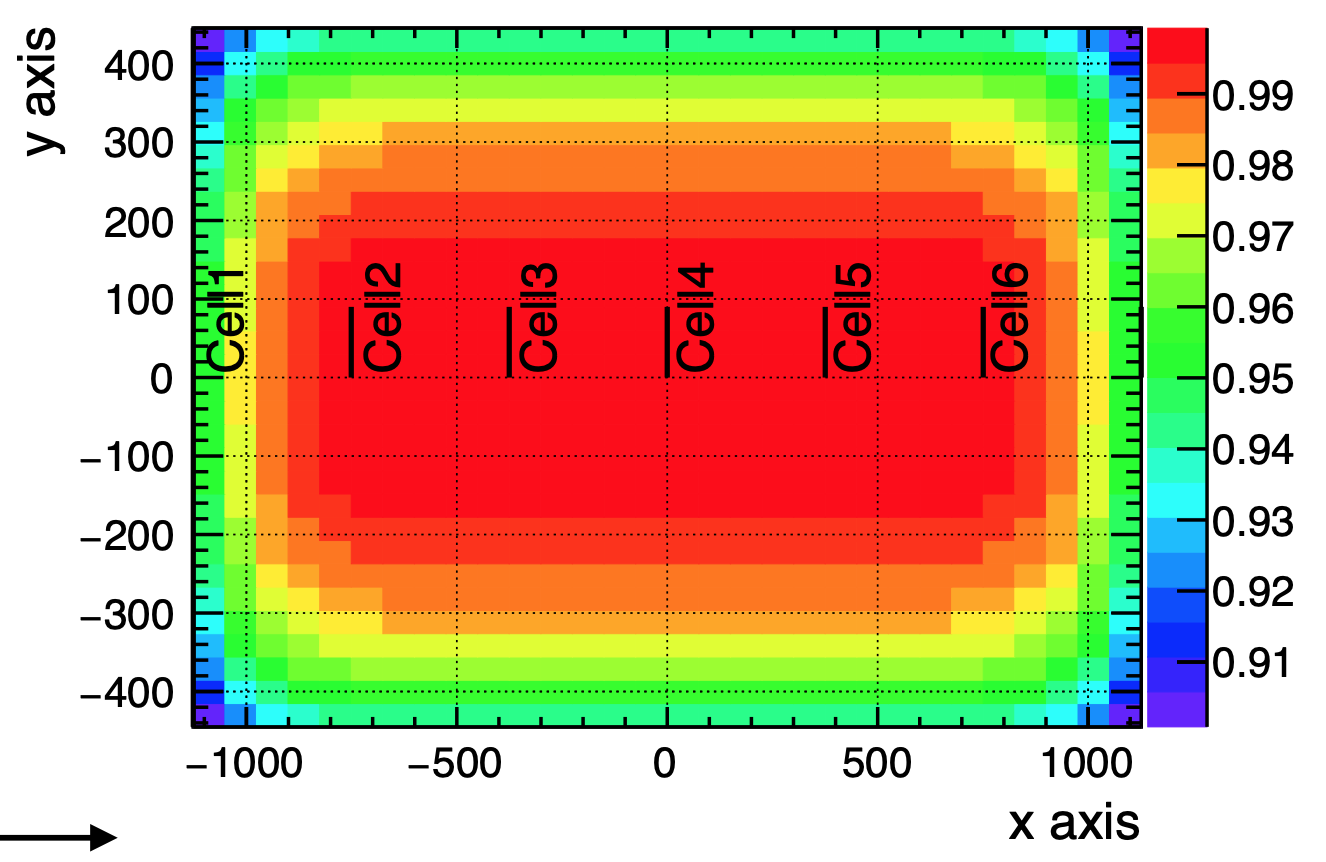
\includegraphics[width=1\linewidth]{images/f_xy_Gd_fraction.png}
\caption{}
\label{fig:f_xy_Gd_fraction.png}

\end{subfigure}
\caption[Ajustement d'un modèle d'évolution du rapport des efficacités de la coupure Retardé entre les données et la simulation]{Ajustement d'un modèle d'évolution du rapport des efficacités de la coupure Retardé entre les données et la simulation. Le modèle est ajusté avec les données de captures des neutrons fournies par la source d'AmBe placé dans chaque cellule (a). Le modèle d'évolution de l'efficacité est étendu en Y (b). (source : \cite{docdb861})}
\label{fig:model_2D_capture_n}
\end{figure}

\clearpage


}

L'implémentation du code FIFRELIN dans la simulation, qui a été décrit dans la section \ref{sec:cascade_Gd_MC}, a permis d'améliorer significativement l'accord en forme des spectres en énergie reconstruite. Les spectres obtenus avec GLG4Sim et FIFRELIN sont confrontés aux véritables données dans la figure \ref{fig:FIFRELIN_vs_GLG4Sim_new.pdf}. La coupure sur l'énergie à $\SI{4.5}{MeV}$ pour l'événement Retardé (G) entraine une perte d'efficacité importante (environ $-20 \%$) qui doit être maîtrisée dans la simulation et les données. Avec GLG4Sim, puisque le pic gadolinium à $\sim \SI{8.5}{MeV}$ est légèrement décalé vers le bas par rapport aux données, l'efficacité de la coupure (C) est plus faible. L'utilisation de FIFRELIN a permis de réduire sensiblement cet écart. L'étude de l'efficacité de détection du neutron est exposée dans le paragraphe suivant, et les nombres présentés correspondent à la comparaison des données avec le modèle fourni par FIFRELIN.\\

La première quantité à comparer avec la simulation est la concentration de gadolinium dans le liquide scintillateur. Celle-ci est caractérisée par la proportion de capture des neutronsiques sur un noyau de gadolinium par rapport au nombre de captures sur hydrogène. Pour ce faire, le rapport entre le nombre de captures sur le gadolinium $N_\textrm{Gd}$ et le nombre de captures total, c'est-à-dire avec l'hydrogène ($N_\textrm{H} + N_\textrm{Gd}$), est mesuré dans les données et la simulation:

\begin{equation}
    f_\textrm{Gd} \doteq \frac{N_\textrm{Gd}}{N_\textrm{H} + N_\textrm{Gd}}.
\end{equation}

\bigbreak

Les quantités $N_\textrm{H}$ et $N_\textrm{Gd}$ sont respectivement représentées par les zones en bleu et en vert sur la figure \ref{fig:Data_z45cm-Delay-Diff-Energy.pdf}. $N_\textrm{H}$ est défini en comptant les événements entre 1,5 et \SI{3}{MeV}, et $N_\textrm{Gd}$ entre 3 et $\SI{10}{MeV}$. L'incertitude sur cette quantité est donnée par la loi binomiale:

\begin{equation}
    \delta f_\textrm{Gd} = \sqrt{\frac{f_\textrm{Gd}(1-f_\textrm{Gd})}{N_\textrm{H} + N_\textrm{Gd}}}.
\end{equation}

\bigbreak

Le rapport $f_\textrm{Gd}(\textrm{Data})/f_\textrm{Gd}(\textrm{MC}) \doteq C_\textrm{Gd}$ exprime les disparités d'efficacité de capture entre les données et la simulation. En pratique, $C_\textrm{Gd}$ est utilisé pour corriger l'efficacité totale de détection du MC $\varepsilon_d^\textrm{tot}$ définie dans le Chapitre \ref{chap:chapitre_3}, Equation (\ref{eq:def_detection_eff}). Néanmoins, les inhomogénéités de ce coefficient entre chaque cellule et chaque position en $z$ doivent être prises en compte pour corriger l'efficacité relative des cellules. Pour ce faire, un modèle d'efficacité de capture 3D a été développé. Les variations de $C_\textrm{Gd}$ suivant l'axe $Z$ sont relativement faibles (les incertitudes couvrent les variations résiduelles) donc un modèle constant est utilisé pour décrire l'évolution de l'efficacité : $C(z) = 1$. Les cellules étant réparties sur l'axe $X$, un modèle $C(x)$ est ajusté en fonction des valeurs de $C_\textrm{Gd}$ pour chaque cellule et moyennées en $z$. $C(x)$ est une fonction de Subbotin  \cite{zbMATH02598645} qui s'écrit sous la forme d'une distribution normale généralisée:

\begin{equation}
    C(x) = \textrm{exp}\left[-\left( \frac{|x - \mu_x|}{\sigma_x} \right)^{\beta_x}\right],
\end{equation}

\bigbreak

avec $\mu_x$, $\sigma_x$ et $\beta_x$ les paramètres à ajuster. Notons qu'avec $\beta_x = 2$, $C(x)$ est une gaussienne et lorsque $\beta_x > 2$, $C(x)$ laisse apparaitre un plateau autour de $\mu_x$. Le résultat de l'ajustement est présenté sur la figure \ref{fig:f_x_Gd_fraction.png}. Les cellules centrales ont une valeur de $C(x)$ similaire, car le déficit de $1\%$ ($C(x) = 99\%$) est principalement causée par l'asymétrie haut-bas. En revanche, on observe une chute d'efficacité avec les cellules 1 et 6 dues à leur proximité avec le Gamma-Catcher. L'effet est plus fort dans la cellule 1 car le tube de calibration est davantage vers l'extérieur. Ce biais résiduel données/MC s'explique par la description de la physique du neutron à basse énergie dans la Gamma-Catcher (effets moléculaires). Ce phénomène est mesuré et pris en compte dans le modèle 3D. Pour ce qui concerne $C(y)$, le système de calibration ne permet pas de sonder la réponse du détecteur suivant cet axe. Cependant, puisqu'\textit{a priori} les chutes d'efficacité sur les bords de la Target sont dues aux mêmes effets physiques qu'en $x$, le modèle en $y$ est paramétré avec $C(x)$:

\begin{equation}
\begin{gathered}
    C(y) = \textrm{exp}\left[-\left( \frac{|y - \Delta l_{xy} - \mu_x|}{\sigma_x} \right)^{\beta_x}\right],\\
    \textrm{avec } \Delta l_{xy} = \left\{
    \begin{array}{l}
        - (\Delta L_x - \Delta L_y)/2 \textrm{ lorsque } y > 0\\
        (\Delta L_x - \Delta L_y)/2 \textrm{ sinon.}
    \end{array}
    \right. .
\end{gathered}
\end{equation}

\bigbreak

Les quantités $\Delta L_x$ et $\Delta L_y$ représentent les dimensions de la Target en $x$ et $y$ respectivement et servent à transposer le modèle suivant les dimensions en $y$. L'évolution de $C_\textrm{Gd}$ en fonction de $x$ et $y$ est visualisée par la figure \ref{fig:f_xy_Gd_fraction.png}. Le modèle d'efficacité final est calculé en faisant le produit : $C_\textrm{Gd}(x,y,z) = C(x)C(y)C(z)$.\\

 Ainsi, la fraction de captures neutrons sur gadolinium d'une cellule peut être obtenue en intégrant $C_\textrm{Gd}(x,y,z)$ sur son volume $V_\textrm{cell}$:

\begin{equation}
    C_\textrm{Gd}(\textrm{cell}) = \frac{1}{V_\textrm{cell}} \iiint_{V_\textrm{cell}} f_n(x,y,z) C_\textrm{Gd}(x,y,z)dxdydz,
\end{equation}

\bigbreak

où $f_n(x,y,z)$ est la densité de probabilité des vertex de création de neutrons. À l'aide des simulations de neutrinos décrites dans la section \ref{sec:neutrino_simulation}, le facteur de correction $C_\textrm{Gd}(\textrm{cell})$ est estimé en bouclant sur les vertex IBD simulés:

\begin{equation}
    C_\textrm{Gd}^\nu(\textrm{cell}) = \frac{1}{N_\nu(\textrm{cell})} \sum_n^{N_\nu(\textrm{cell})} C_\textrm{Gd}(x_n,y_n,z_n),
\end{equation}

\bigbreak

avec $N_\nu(\textrm{cell})$ le nombre de neutrons créés dans la cellule en question et $x_n$, $y_n$ et $z_n$ la position du vertex d'émission du neutron $n$. Ce sont ces facteurs de corrections $C_\textrm{Gd}^\nu$ qui interviennent lors de l'analyse d'oscillation pour que les cellules de la simulation aient la même efficacité de détection relative. Les valeurs de $C_\textrm{Gd}^\nu$ pour chaque cellule sont rassemblées dans le Tableau \ref{tab:data_mc_gd_fraction_ratios}.\\


\afterpage{

\begin{table}[h!]
  \begin{center}
    \begin{tabular}{|c|c|c|c|c|c|c|}
    \hline
      Cellule & 1 & 2 & 3 & 4 & 5 & 6\\
      \hline
      \hline
      $C_\textrm{Gd}^\nu$ & 0,9653 & 0,9845 & 0,9848 & 0,9848 & 0,9845 & 0,9660\\
      \hline
      $\left<C_\textrm{Retardé}\right>_{\textrm{cells},z}$ & \multicolumn{6}{c|}{1.0072}\\
      \hline
      $C_\textrm{total}^\nu$ & 0,9723 & 0,9916 & 0,9919 & 0,9918 & 0,9916 & 0,9729 \\
      \hline
    \end{tabular}
  \end{center}
  \caption[Disparités d'efficacité de capture n-Gd entre les données et la simulation]{Disparités d'efficacité de capture n-Gd entre les données et la simulation. $C_\textrm{Gd}^\nu$ représentent l'écart donnée/MC sur la fraction de captures neutrons sur gadolinium, tandis que $\left<C_\textrm{Retardé}\right>_{\textrm{cells},z}$ est l'efficacité moyenne entre cellules et position en $z$ de la coupure sur l'événement Retardé. $C_\textrm{total}^\nu$ est le produit de ces deux quantités. Ce sont ces valeurs qui sont utilisées pour renormaliser les spectres neutrinos dans la simulation. (source : \cite{docdb945})}
    \label{tab:data_mc_gd_fraction_ratios}
\end{table}

}

\bigbreak

\subsubsection*{Efficacité des coupures topologiques et temporelles}

\afterpage{

\begin{figure}[h!]
\centering
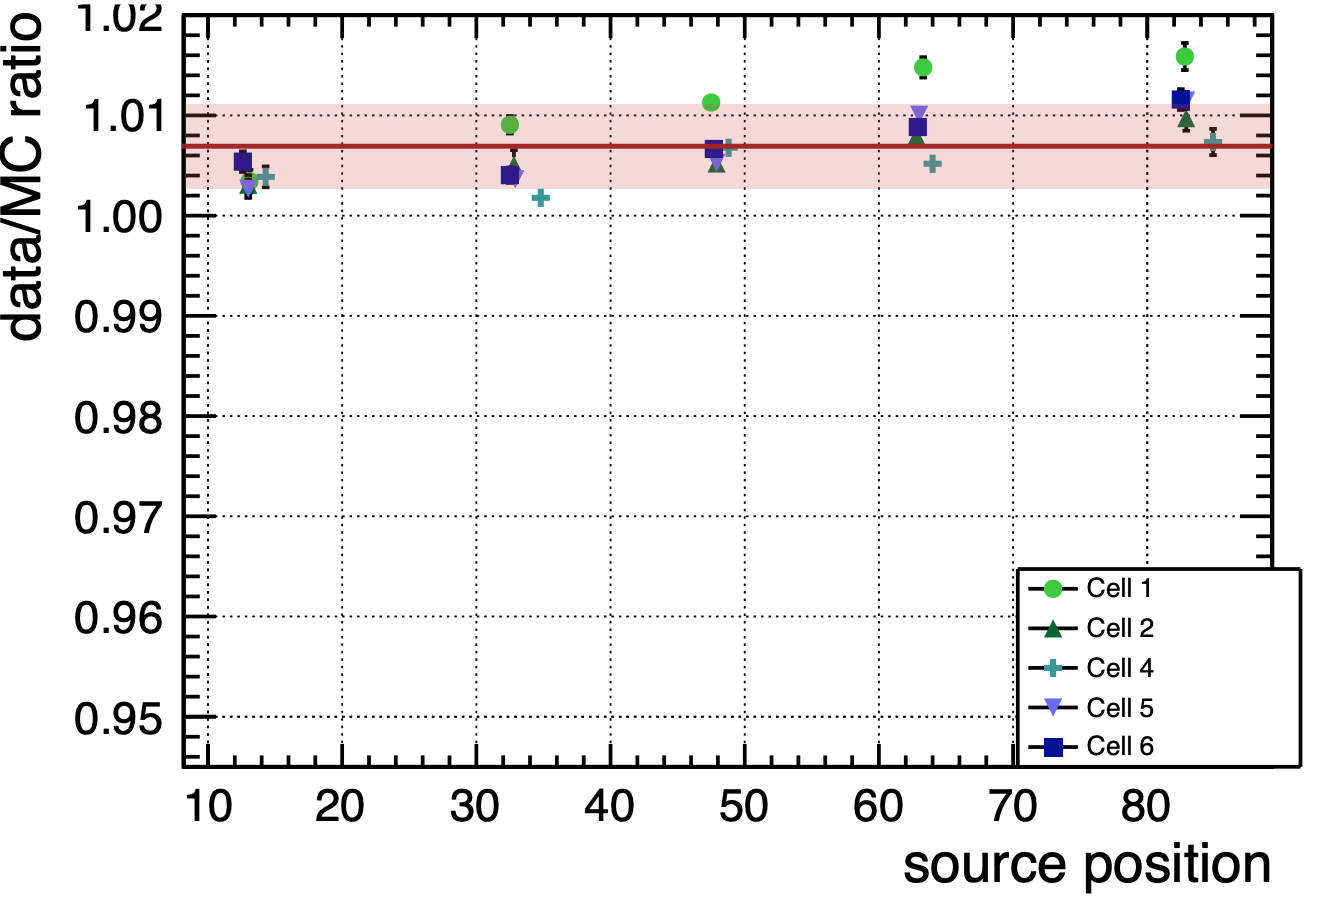
\includegraphics[width=0.8\textwidth]{images/IBD_cuts_eff_inhomo.png}
\caption[Inhomogénéités des rapports d'efficacité entre les données et la simulation]{Inhomogénéités des rapports d'efficacité entre les données et la simulation. (source : \cite{docdb861})}
\label{fig:IBD_cuts_eff_inhomo.png}

\end{figure}

}

L'efficacité des coupures sur l'énergie reconstruite de l'événement Retardé et sur le temps de latence Prompt-Retardé $\Delta T$ est obtenue en faisant le rapport du nombre d'événements avec et sans coupure:

\begin{equation}
\begin{gathered}
    \varepsilon_\textrm{Retardé} \doteq \frac{N\left( 4.5 < E^\textrm{rec} < \SI{10}{MeV} \textrm{ et } E^\textrm{rec}_\textrm{Target} > \SI{1}{MeV} \textrm{ et } 2 < \Delta T < \SI{70}{\mu s}  \right)}{N_\textrm{Gd}}, \\
    \textrm{ et } \delta \varepsilon_\textrm{Retardé} = \sqrt{\frac{\varepsilon_\textrm{Retardé}(1-\varepsilon_\textrm{Retardé})}{N_\textrm{Gd}}}.
\end{gathered}
\end{equation}

\bigbreak

Cette quantité est calculée à la fois dans les données et dans la simulation pour chaque position de la source d'AmBe (hauteur et cellule). Le rapport moyen $C_\textrm{Retardé} \doteq \varepsilon_\textrm{Retardé} (\textrm{Données}) / \varepsilon_\textrm{Retardé} (\textrm{MC})$ donne le facteur de correction à appliquer sur la normalisation des spectres neutrinos, et son incertitude associée se propage dans le bilan d'erreurs. Sa valeur moyennée sur toutes les positions est de $\left<C_\textrm{Retardé} \right>_{\textrm{cells},z} = (100,72 \pm 0,38) \%$ \cite{docdb945}. L'erreur sur la moyenne est calculée en prenant la déviation standard des $C_\textrm{Retardé}(\textrm{cell}, z)$ individuels. La figure \ref{fig:IBD_cuts_eff_inhomo.png} montre la répartition des valeurs de $C_\textrm{Retardé}$ en fonction de $z$, pour chaque cellule. Finalement, le désaccord d'efficacité de détection du neutron entre les données et le MC est obtenu en multipliant : $\left<C_\textrm{Retardé} \right>_{\textrm{cells},z} \times C^\nu_\textrm{Gd}(i) \doteq C^\nu_\textrm{Total}(i)$, où $i$ est le numéro de la cellule considérée. Les valeurs de $C^\nu_\textrm{Total}(i)$ qui sont écrites dans le Tableau \ref{tab:data_mc_gd_fraction_ratios} servent en définitive à renormaliser les spectres d'énergie des positrons de chaque cellule dans la simulation.\\

\subsubsection*{Estimation des incertitudes systématiques}

\afterpage{

\begin{table}[h!]
  \begin{center}
    \begin{tabular}{|c|c|c|}
    \hline
      Incertitude & $\delta C_\textrm{Gd}^\nu$ & $\delta  \left<C_\textrm{Retardé}\right>_{\textrm{cells},z}$ \\
      \hline
      \hline
      Variation temporelle & \multicolumn{2}{c|}{$\pm 0,10 \%$} \\
      \hline
      Position de la source en $z$ & $\pm 0,22 \%$ & $\pm 0,27 \%$ \\
      \hline
      Homogénéité & $\pm 0,51 \%$ & $\pm 0.,38 \%$\\
      \hline
      Total & $\pm 0,56 \%$ & $\pm 0,48 \%$\\
      \hline
    \end{tabular}
  \end{center}
  \caption[Liste des erreurs systématiques associées aux coefficients traitants de l'efficacité de détection des neutrons]{Liste des erreurs systématiques associées aux coefficients traitants de l'efficacité de détection des neutrons : $C_\textrm{Gd}^\nu$ et $\left<C_\textrm{Retardé}\right>_{\textrm{cells},z}$.}
    \label{tab:gd_correction_factor_uncertainty}
\end{table}

}

Les erreurs systématiques associées à ces nombres ont été estimées via trois facteurs : l'évolution en temps, les biais dus à la mauvaise position de la source en $z$, et les inhomogénéités. Ces analyses avec l'AmBe ont été menées sur toutes les campagnes de calibration, et les variations temporelles de $C_\textrm{Retardé} (\textrm{cell},z)$ et $C^\nu_\textrm{Gd}(\textrm{cell},z)$ sont de $0,1 \%$ à $1\sigma$ chacun. Par ailleurs, la position de la source en $z$ est repérée par une étiquette disposée sur le câble au bout duquel se trouve le porte source. L'incertitude sur la position des étiquettes a été considérée à $\pm \SI{1}{cm}$. En appliquant un biais de $\SI{1}{cm}$ sur la hauteur en $z$ dans la simulation les quantités $C_\textrm{Retardé} (\textrm{cell},z)$ et $C^\nu_\textrm{Gd}(\textrm{cell},z)$ évoluent de $\pm 0,22 \%$ et $\pm 0,27 \%$ respectivement. Enfin, les inhomogénéités du coefficient $C^\nu_\textrm{Gd}(\textrm{cell},z)$ induisent une erreur sur les paramètres du modèle 3D. En effet le modèle en $z$ a été choisi constant ($C(z) \doteq 1$) alors que la fraction de captures sur Gd ($C^\nu_\textrm{Gd}(\textrm{cell},z)$) présente une légère évolution. L'incertitude associée à cette grandeur a été estimée à $\pm 0,51 \%$.\\

L'incertitude totale sur les coefficients est calculée par somme quadratique de ces 3 composantes. Ces erreurs sont finalement propagées sur les spectres positrons pour l'analyse statique qui est discutée dans le Chapitre \ref{chap:chapitre_stat}. Le Tableau \ref{tab:gd_correction_factor_uncertainty} est un compendium des incertitudes systématiques associées à ces coefficients.

\bigbreak

\section{Recherche de paires corrélées en temps}

À la manière des expériences pionnières de Cowan et Reines \cite{Reines:1953kf}, l'identification d'une IBD est effectuée par la double détection de deux signaux Prompt et Retardé, dans un intervalle de temps restreint. Dans un premier temps le principe de la recherche de paire et l'application des coupures est discuté, suivi d'une partie consacrée à la soustraction des coïncidences fortuites (accidentelles). Enfin le calcul du temps mort est brièvement mentionné pour terminer sur les tests menés pour valider l'algorithme.

\subsection{Principe de la méthode de recherche de paires}

L'algorithme de recherche de paires corrélées en temps consiste à sélectionner des paires d'événements qui respectent un certain nombre de contraintes : énergie, écart en temps, confinement géométrique de la paire. Cette méthode a également pour but de soustraire la composante de bruits de fond dits accidentels, qui relève de sa nature purement statistique.\\

Deux algorithmes de recherches de paires ont été développés indépendamment au sein de la collaboration. Bien que leur principe de fonctionnement est similaire, l'intérêt de paralléliser cette tâche repose sur deux constats: l'élaboration de tels programmes est complexe et nécessite un travail d'optimisation réfléchi; de plus, les erreurs d'exécution sont parfois subtiles, car les éléments en sortie peuvent contenir des biais sans pour autant présenter des résultats aberrants. La vérification croisée des deux codes assure donc une fiabilité capitale pour l'extraction des taux de comptage des candidats neutrinos. La méthode décrite ici est celle développée à Saclay, dans le cadre de la thèse d'Aurélie Bonhomme \cite{bonhomme:tel-01931309}.\\

Les événements de chaque run d'acquisition sont parcourus séquentiellement par le programme qui teste l'ensemble des conditions de topologies décrites dans la section précédente. Inspiré de l'expérience antécédente \textsc{Nucifer} (\cite{pequignot:tel-01217946} et \cite{gaffiot:tel-00770675}), l'algorithme est basé sur l'utilisation d'une mémoire glissante contenant les informations de 4 candidats à la suite: Pré-Prompt, Prompt, Retardé, Post-Retardé. Les runs neutrino sont lus du début à la fin en déplaçant cette fenêtre sur chaque événement. À chaque séquence, le programme vérifie les conditions d'acceptation d'une paire candidate Prompt-Retardé :\\

\begin{itemize}
    \item Les candidats \textbf{Pré-Prompt} et \textbf{Post-Delayed} ne sont pas précédés par un muon : coupures (L) et (M)
    \item Le candidat \textbf{Prompt} respecte les coupures en énergie : (A), (B), (C), (D), (E) et (F)
    \item Le candidat \textbf{Retardé} respecte les coupures en énergie (G), (H) et (I)
    \item Les candidats \textbf{Prompt} et \textbf{Retardé} sont corrélés en distance (J)
    \item L'événement \textbf{Prompt} est suffisamment éloigné de \textbf{Pré-Prompt} (N)
    \item L'événement \textbf{Prompt} est suffisamment éloigné de \textbf{Post-Retardé} (O)
\end{itemize}

\bigbreak

Si l'ensemble des critères est satisfait, alors la paire est stockée dans une base de donnés réduite. Cette collection d'événements se compose de 3 catégories : les événements induits par les neutrinos, les paires de bruits de fond corrélés et les bruits de fond accidentels. Il est important de noter qu'après cette étape, les signaux ne seront plus considérés comme des candidats individuels. En effet les procédures de soustraction des bruits de fond vont s'appliquer sur des distributions, par exemple des spectres en énergie ou PSD, et donc l'information événement par événement ne sera plus accessible.

\bigbreak



%\begin{itemize}
%    \item Algo recherche paires
%    \item soustraction accidentelles
%    \item Calcul du temps effectif
%    \item Cross-check avec pseudo-expériences
%    \item Correction de biais
%\end{itemize}

\subsection{Soustraction de la composante des paires accidentelles}

\label{seq:acc_subtraction}

La contribution des bruits de fond accidentels est mesurée très précisément grâce à la méthode des portes décalées en temps. À chaque paire candidate qui respecte les critères de sélection, un événement Prompt virtuel est créé dans la séquence de données. Ce signal factice est placé $\SI{1}{ms}$ dans le futur par rapport au candidat Prompt original, et l'ensemble des coupures est de nouveau sollicité pour tester s'il se retrouve \textit{accidentellement} associé à un candidat Retardé réel dans les données. Si la paire (ou plus précisément le quatuor à cause des conditions d'isolation) est acceptée, alors un compteur d'accidentelles $N_\textrm{acc}$ est incrémenté. La fenêtre d'$\SI{1}{ms}$ a été choisie suffisamment grande afin de s'affranchir de toute corrélation résiduelle. En pratique, 100 candidats virtuels ($N_\textrm{réinsertions}$) sont chacun placés à $\SI{1}{ms}$ d'intervalle pour obtenir une estimation plus précise du nombre de coïncidences accidentelles. Le principe de cette méthode est résumé sur la figure \ref{fig:acc_method.png}.\\

\afterpage{
% neutron_delta_t_AmBe.pdf

\begin{figure}[h!]
\centering
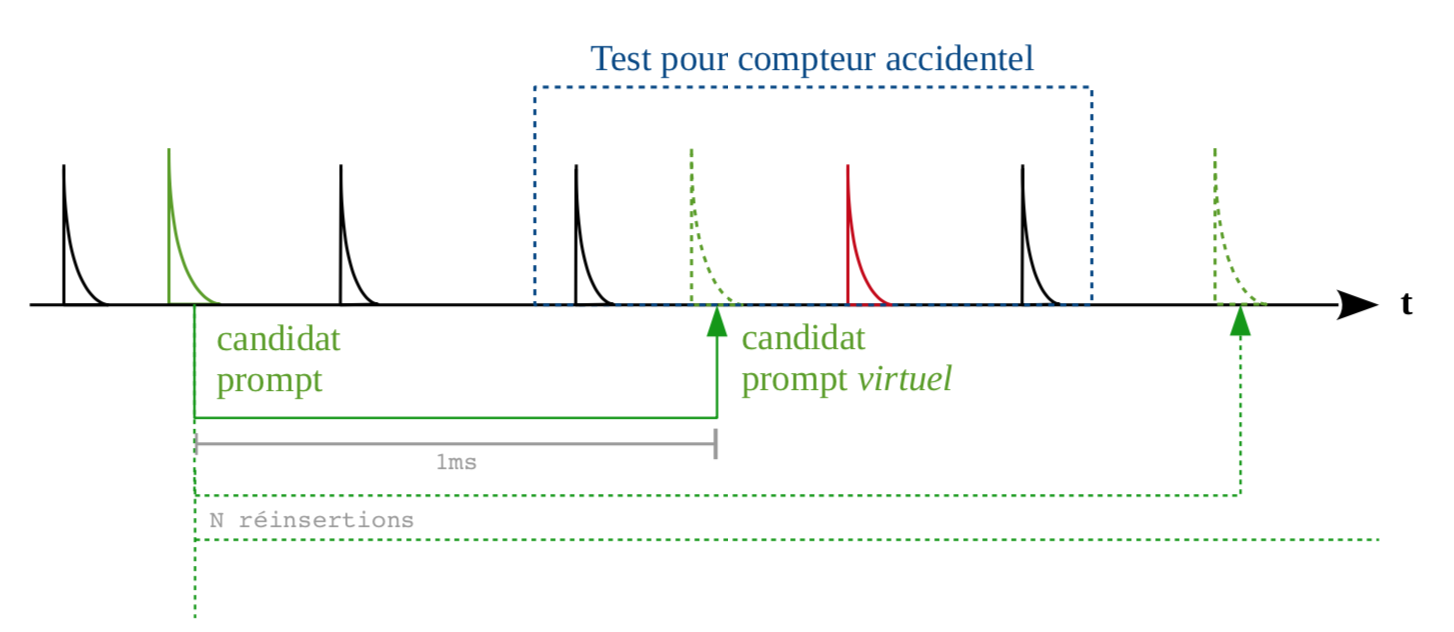
\includegraphics[width=1\textwidth]{images/acc_method.png}
\caption[Méthode de soustraction des bruits de fond accidentels]{Méthode de soustraction des bruits de fond accidentels.}
\label{fig:acc_method.png}

\end{figure}

}

Malgré le fait que toutes des coupures de sélection soit appliquées sur les paires virtuelles comme sur les paires candidates, des facteurs de corrections doivent prendre en compte que la probabilité de former une paire accidentelle est légèrement plus faible. Le premier facteur de correction concerne la coupure véto muon (\ref{eq:cut_muon_veto}). En effet, cette condition s'applique à la fois sur l'événement Prompt et sur le Retardé dans le cas d'une véritable paire corrélée. Étant donné que la coupure véto muon (L) est appliqué sur le Prompt, l'acceptation de l'événement Retardé ne dépend que de l'éventualité où un muon s'insère entre les deux candidats. La probabilité d'acceptation du candidat Retardé est donc fonction de l'intervalle de temps $\Delta T$ (K) et non $\Delta T_\mu$ comme le suggère la coupure (L). En revanche dans le cas de la paire virtuelle, le véto muon n'est appliqué que sur l'événement Retardé donc cette fois la probabilité d'acceptation dépend bien de $\Delta T_\mu$. Le facteur de correction s'exprime donc de la façon suivante:

\begin{equation}
    f^\mu_\textrm{acc} = \frac{P_\mu(\Delta T)}{P_\mu(\Delta T_\mu)} = e^{-R_\mu (\Delta T - \Delta T\mu)},
\end{equation}

\bigbreak

où $P_\mu(\Delta T_\mu)$ et $P_\mu(\Delta T)$ expriment selon des lois poissoniennes, la probabilité de ne pas avoir de muon dans l'intervalle spécifié, et $R_\mu$ le taux de muon observés. Notons que ce facteur de renormalisation n'est appliqué que si la coupure en $\Delta T_\mu$ est plus grande que la fenêtre Prompt-Retardé $\Delta T$.

\bigbreak

Pareillement au véto muon, les coupures d'isolation (N) et (O) induisent un biais sur le calcul des accidentelles. Cette fois, la condition d'isolation du candidat Prompt réinséré est appliquée bien que le candidat Prompt original l'ai déjà satisfaite. Le facteur de correction s'exprime donc ainsi:

\begin{equation}
    f^\textrm{isol}_\textrm{acc} = \frac{P_\textrm{isol} (\Delta T_\textrm{isol}^\textrm{before})}{\left(P_\textrm{isol} (\Delta T_\textrm{isol}^\textrm{before})\right)^2} \times \frac{P_\textrm{isol} (\Delta T_\textrm{isol}^\textrm{after})}{\left(P_\textrm{isol} (\Delta T_\textrm{isol}^\textrm{after})\right)^2} = e^{R_s (\Delta T_\textrm{isol}^\textrm{before} + \Delta T_\textrm{isol}^\textrm{after})},
\end{equation}

\bigbreak

où $R_s$ est le taux de comptage d'événements simples. La probabilité d'acceptation pour l'événement virtuel est élevée au carré parce que la coupure temporelle est en fait appliquée deux fois : une fois par l'événement Prompt original, et une fois par l'événement virtuel. Ainsi, le facteur de correction global à appliquer sur l'estimation des coïncidences fortuites est défini de la sorte :

\begin{equation}
    f_\textrm{acc}(\Delta T) \doteq \frac{f^\mu_\textrm{acc} (\Delta T) f^\textrm{isol}_\textrm{acc}}{N_\textrm{réinsertions}}.
\end{equation}

\bigbreak

Remarquons que la dépendance en $\Delta T$ est précisée, car cela implique un facteur de correction différent pour chaque paire. En pratique $f_\textrm{acc}$ est estimé pour chaque bin en $\Delta T$ et sa dépendance n'est considéré que pour estimer la distribution en $\Delta T$ des événements corrélés. Du reste, seule la valeur moyenne $\left< f_\textrm{acc} \right>_{\Delta T} $ est utilisée pour soustraire les distributions dont la composante accidentelle est indépendante de $\Delta T$.\\

Finalement, le taux de paires corrélées est estimé par soustraction des bruits de fond accidentels de la façon suivante:

\begin{equation}
    N_\textrm{corr} = N_\textrm{corr + acc} - N_\textrm{acc} \left< f_\textrm{acc} \right>_{\Delta T}.
\end{equation}

\bigbreak

\subsection{Calcul du temps d'acquisition effectif}

Afin de convertir le nombre de coïncidences corrélées mesuré $N_\textrm{corr}$ en taux de comptage, le temps mort de chaque run doit être estimé. Le temps mort induit par les coupures d'isolation temporelle (N) et (O) est largement dominant face à celui induit par l'électronique ($< 0.2 \%$). La procédure  d'estimation du temps d'acquisition effectif fait intervenir les probabilités d'occurrence des événements. Celle-ci est brièvement résumée dans les paragraphes suivants. Pour plus de détails, le lecteur se réfèrera au manuscrit de thèse d'Aurélie Bonhomme \cite{bonhomme:tel-01931309}.\\

Chaque paire d'événements provoque un certain temps mort d'acquisition. Par exemple, la détection d'un candidat muon empêche la détection d'un neutrino pendant un laps de temps défini par les coupures d'isolation. La fraction de temps mort $f_\textrm{dead}$ à laquelle la détection d'un événement est soumise peut être écrite en fonction du taux de comptage des événements contribuant au temps mort $R$ et du temps mort moyen induit par ces derniers $\overline{\tau}$ :

\begin{equation}
    f_\textrm{dead} = R\overline{\tau}.
\end{equation}

\bigbreak

Cette grandeur donne le pourcentage de temps pendant lequel l'acquisition ne peut mesurer un signal. Dans le cas des neutrinos, le signal a une largeur temporelle qui est l'écart entre l'arrivée de l'événement Prompt et du Retardé. Un facteur de correction doit être appliqué:

\begin{equation}
    f_\textrm{dead}^\textrm{pair} = f_\textrm{dead} + \left<\Delta T\right>_\textrm{pairs} R_\mu e^{-R \Delta T_\mu},
\end{equation}

\bigbreak

où $R_\mu$ et $\Delta T_\mu$ sont respectivement le taux de comptage de muons et la coupure d'isolation des muons. Le principe de cette correction est illustré sur la  figure \ref{fig:dead_time_correction.png}. En définitive, le nombre de paires d'événements corrélés est converti en taux de comptage avec le temps d'acquisition $T_\textrm{run}$ et la fraction de temps mort associée aux paires corrélées:

\begin{equation}
    R_\textrm{corr} = \frac{N_\textrm{corr}}{T_\textrm{run}\left(1 - f_\textrm{dead}^\textrm{pair} \right)}.
\end{equation}


% Pour chaque type d'événements étiqueté $i$, qui à la détection sans chevauchement créé un temps mort $\Delta T_i$, le temps mort moyen peut être exprimé comme suit:

%\begin{equation}
%    \overline{\tau}_i = \int_{0}^{\infty} P(t) \tau dt,
%\end{equation}
%
%\bigbreak
%
%où $P(t)$ désigne la densité de probabilité qu'un nouvel événement de type $i$ soit détecté après un laps de temps égal à $t$ et $\tau$ le temps mort qu'il induit. Si $t$ est plus grand que $\Delta T_i$ alors $\tau$ prend cette valeur, sinon, cela signifie qu'il y a un recouvrement entre deux événements de type $i$, et le temps mort est $\tau = t$:
%
%\begin{equation}
%    \overline{\tau}_i = \int_{0}^{\Delta T_i} P(t) t dt + \int_{\Delta T_i}^{\infty} P(t) \Delta T_i dt.
%\end{equation}
%
%\bigbreak
%
%En considérant que les événements $i$ soient générés suivant une loi poissonienne, la densité de probabilité est $ P(t) = R_i e^{-R_it} $, où $R_i$ est le taux de comptage associé à $i$. Le temps mort moyen devient:
%
%\begin{equation}
%    \overline{\tau}_i = \frac{1}{R_i} \left(1 - e^{-R_i\Delta T_i}\right).
%\end{equation}
%
%\bigbreak
%
%Cette formule peut être généralisée en considérant $n$ types d'événements enchevêtré. Le temps mort moyen total est:
%
%\begin{equation}
%\label{eq:total_mean_dead_time}
%    \overline{\tau} = \frac{1}{R}\sum_{i = 1}^{n} \frac{R_i}{R} \left(1 - e^{-R\Delta T_i}\right),
%\end{equation}
%
%\bigbreak
%
%où $R \doteq \sum_i R_i$ est le rate total des événements contribuant au temps mort \cite{bonhomme:tel-01931309}. Dans le cas de la recherche de paires neutrinos, deux types d'événements contribuent au temps mort: les vétos muon (L) et les conditions d'isolation temporelle de la paire avec un bruit de fond Simple (N) et (O). La fraction de temps mort de l'acquisition  s'exprime finalement comme:
%
%\begin{equation}
%    X_\textrm{dead} \doteq R\overline{\tau} = \frac{1}{R_\mu + R_s}\left\{ R_\mu\left(1 - e^{-(R_\mu + R_s)\Delta T_\mu}\right) + R_s \left(1 - e^{-(R_\mu + R_s)(\Delta T_\textrm{isol}^\textrm{before} + \Delta T_\textrm{isol}^\textrm{after})} \right)\right\} ,
%\end{equation}
%
%\bigbreak

% où $R_\mu$ est le taux de muons, $R_s$ le taux d'événements Simples. Cette grandeur donne le pourcentage pendant lequel l'acquisition ne peut mesurer un signal. Dans le cas des neutrinos, le signal a une largeur temporelle qui est l'écart entre l'arrivée de l'événement Prompt et du Retardé (voire figure \ref{fig:dead_time_correction.png}). Un facteur de correction doit être appliqué:

%\begin{equation}
%    X_\textrm{dead}^\textrm{pair} = X_\textrm{dead} + \left<\Delta T\right>_\textrm{pairs} R_\mu e^{-(R_\mu + R_s) \Delta T_\mu}.
%\end{equation}

\afterpage{

\begin{figure}[h!]
\centering
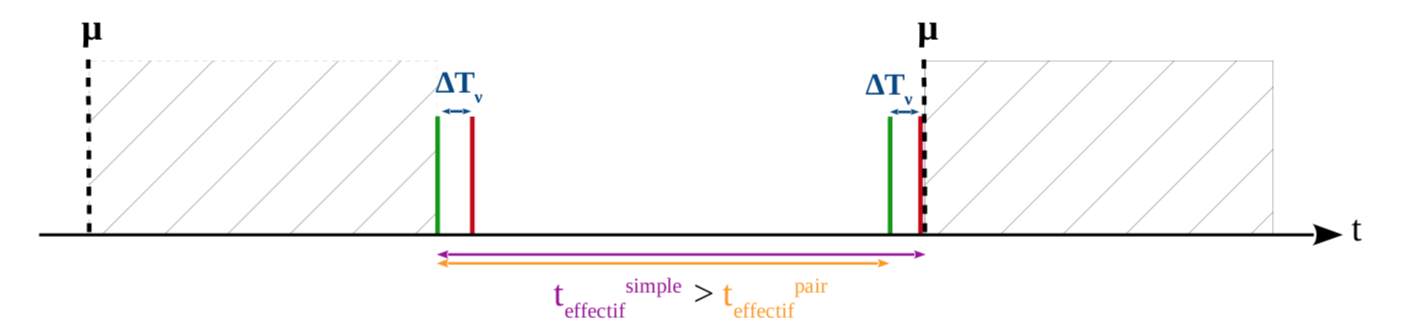
\includegraphics[width=1\textwidth]{images/dead_time_correction.png}
\caption[Illustration de la correction à appliquer sur le temps mort pour la recherche de paires corrélées.]{Illustration de la correction à appliquer sur le temps mort pour la recherche de paires corrélées. Le temps d'acquisition effectif est plus faible dans le cas des paires corrélées à cause de l'étalement temporel de ces dernières. (source : \cite{bonhomme:tel-01931309})}
\label{fig:dead_time_correction.png}

\end{figure}

}

%\bigbreak
%
%En définitive, le nombre de paires d'événements corrélé est converti en taux de comptage avec le temps d'acquisition $T_\textrm{run}$ et la fraction de temps mort associée aux paires corrélées:
%
%\begin{equation}
%    R_\textrm{corr} = \frac{N_\textrm{corr}}{T_\textrm{run}\left(1 - X_\textrm{dead}^\textrm{pair} \right)}.
%\end{equation}


\bigbreak

\subsection{Validation de l'algorithme}

Afin d'affirmer le bon comportement de l'algorithme dans la recherche de paires, la soustraction du bruit de fond accidentel, et le calcul des \textit{rates}, une séquence de données a été générée par simulation. Ce jeu de données simulées est composé des différents types de bruits de fond auquel est soumise l'expérience. Chacun d'eux est généré indépendamment suivant une loi de probabilité telle que $P(t) \propto e^{R_it}$, où $R_i$ est le taux d'occurrences du type de bruit de fond considéré. Les différents types d'événements générés sont:\\

\begin{itemize}
    \item des signaux isolés dits Simples, suivant un taux de comptage $R_s$,
    \item des signaux isolés dits Muons, suivant un taux de comptage $R_\mu$,
    \item des signaux isolés dits Prompts (c'est-à-dire qui passent les coupures topologiques associées au Prompt), suivant un taux de comptage $R_p$,
    \item des signaux isolés dits Retardés (idem pour les coupures sur l'événement Retardé), suivant un taux de comptage $R_r$,
    \item des paires d'événements corrélés Prompt-Retardé, avec un taux d'occurrence $R_c$.
\end{itemize}

\bigbreak

Plusieurs jeux de données simulés sont générés sous forme de runs d'une heure, comme les véritables données. L'algorithme est testé avec des taux de comptages qui varient de run à run; le but étant de retrouver la fréquence d'événements corrélés qui a été injectée: $R_c$.\\

\afterpage{

%acc_only_test.png

\begin{figure}[h!]
\centering
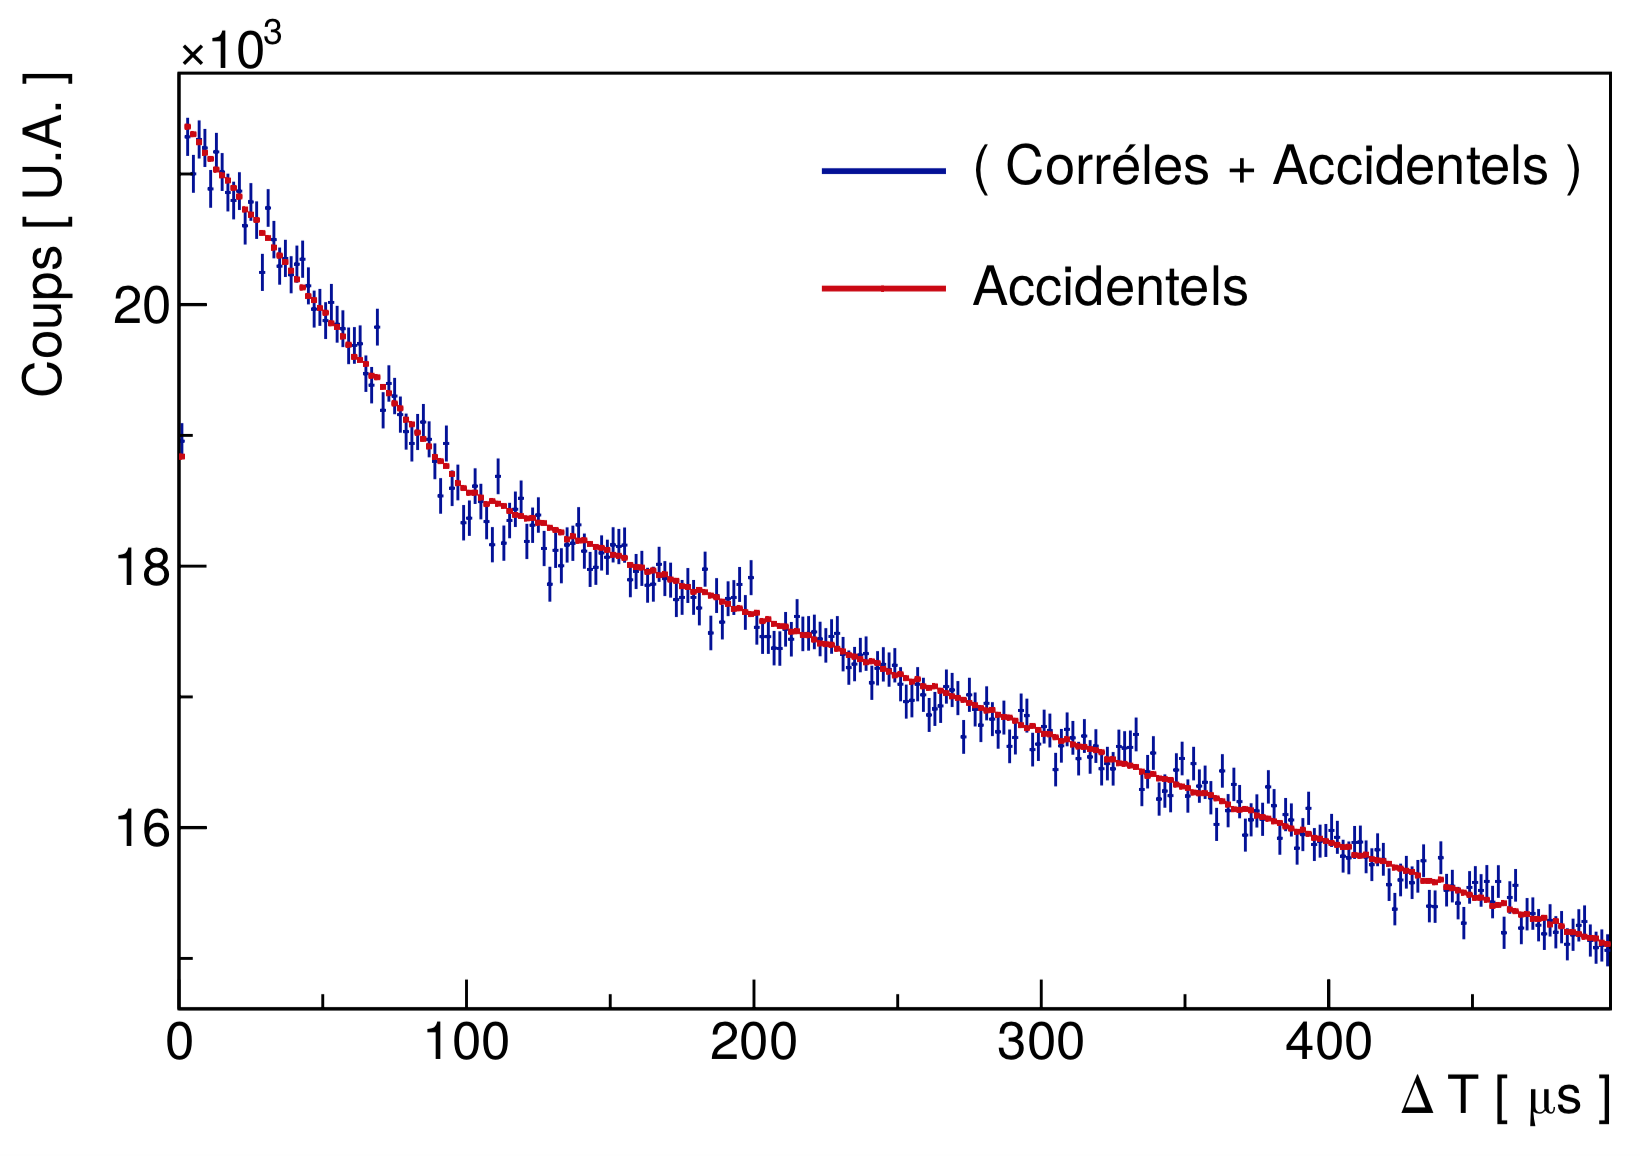
\includegraphics[width=0.7\textwidth]{images/acc_only_test.png}
\caption[Mise à l'épreuve de la méthode de soustraction des paires accidentelles]{Mise à l'épreuve de la méthode de soustraction des paires accidentelles. Dans cette pseudo-expérience, seuls des candidats simples ont été injectés. L'estimation du nombre de paires accidentelles (rouge) doit donc correspondre avec les coincidences obtenues en appliquant l'algorithme de recherche de paires (bleu). (source : \cite{bonhomme:tel-01931309})}
\label{fig:acc_only_test.png}

\end{figure}

% ultimate_test_corr_acc_var.png

\begin{figure}[h!]
\centering
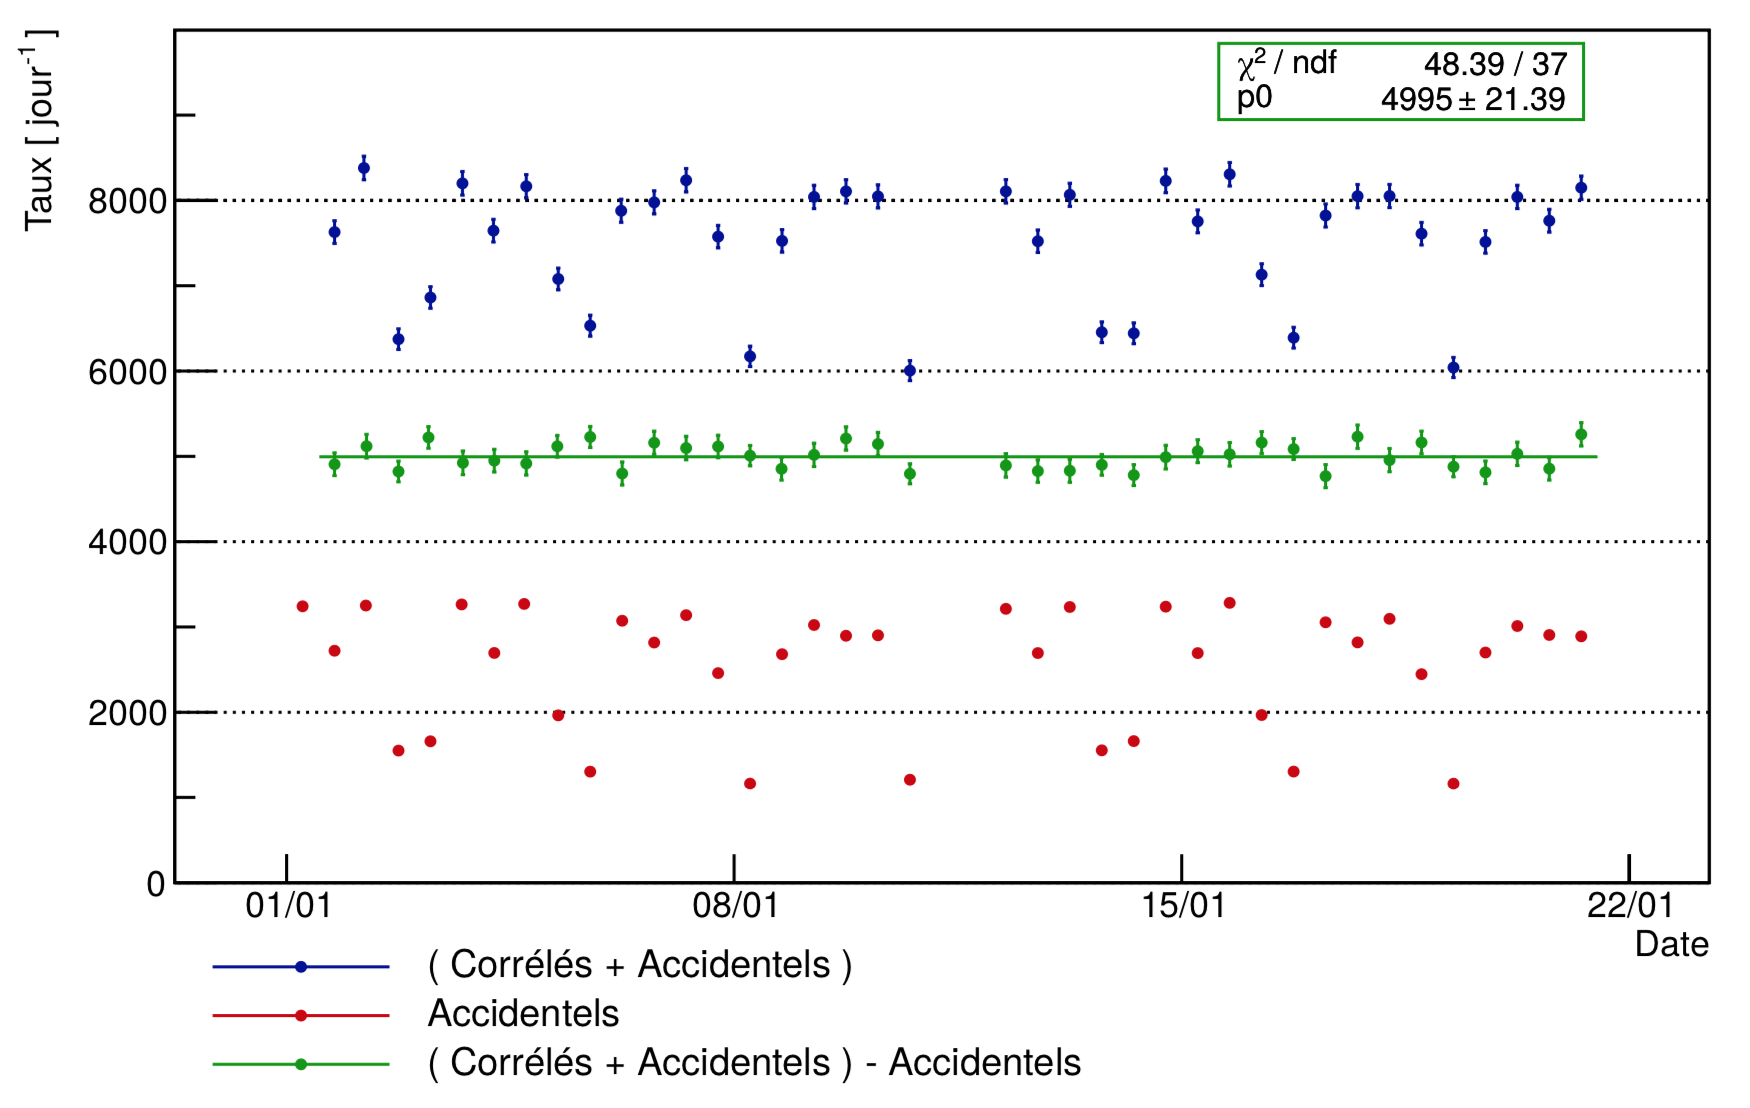
\includegraphics[width=0.7\textwidth]{images/ultimate_test_corr_acc_var.png}
\caption[Test de robustesse complet de l'algorithme de recherche de paires corrélées en temps]{Test de robustesse complet de l'algorithme de recherche de paires corrélées en temps. Malgré les importantes variations du taux d'accidentelles, le taux de paires corrélées mesuré coïncide avec la valeur injectée : 5000/jour. (source : \cite{bonhomme:tel-01931309})}
\label{fig:acc_only_test.png}

\end{figure}

}

La procédure de soustraction des accidentelles a dans un premier temps été testée en ne générant que des événements non corrélés, c'est-à-dire $R_c = 0$. L'analyse a montré des résultats satisfaisants présentés sur la figure \ref{fig:acc_only_test.png}. La rupture de pente observée sur la distribution des $\Delta T$ est causée par la coupure véto muon (L). La probabilité de former une paire $p(\Delta T)$ change de comportement suivant si l'écart en temps Prompt-Retardé est plus petit ou plus grand que le véto muon.\\

Un test plus complet a aussi été effectué en générant l'équivalent de trente jours de données \textsc{Stereo} en modulant fortement l'amplitude du taux de candidats type $R_s$, $R_\mu$, $R_p$ et $R_r$. La figure \ref{fig:acc_only_test.png} montre l'évolution en temps du taux de paires corrélées reconstruites. Malgré les importantes variations des paires accidentelles, l'algorithme démontre sa capacité à reconstruire le taux de paires corrélées $R_c$ injecté avec la précision indiquée par les barres d'erreurs. Cette mise à l'épreuve sollicite à la fois la méthode de soustraction des bruits de fond accidentels, mais aussi les corrections de temps mort.\\

\bigbreak

\section{Extraction des spectres neutrinos}

Une fois la recherche de paires et la soustraction des bruits de fond accidentels effectuées, les distributions obtenues comportent le signal neutrino, mais aussi les bruits de fond corrélés. La soustraction de cette dernière composante nécessite de la mesurer seule, c'est-à-dire d'utiliser les données acquises lorsque le réacteur est OFF. En principe, la soustraction des spectres en énergie ON-OFF devrait suffire pour extraire les spectres neutrinos. Cependant malgré les critères de sélection et la recherche de paires, la contribution des bruits de fond corrélés ($R_c$) reste importante face au signal neutrino ($R_\nu$) et l'erreur induite par la procédure de soustraction est essentiellement dominée par l'erreur statistique du bruit:

\begin{equation}
    \delta R_\nu = \delta ((R_\nu + R_c) - R_c) = \delta (R_\nu + R_c) \oplus \delta R_c = \delta R_{ON} \oplus \delta R_{OFF},
\end{equation}

\bigbreak

où $R_{ON}$ et $R_{OFF}$ sont respectivement les taux de comptages de paires corrélées lorsque le réacteur est ON ou OFF.\\

Pour s'affranchir d'une grande partie des bruits de fond corrélés, la discrimination en forme des signaux (PSD) est exploitée. En effet, la majorité des bruits de fond corrélé est d'origine cosmique, et donc principalement composé de neutrons issus de réactions de spallation.

\bigbreak

\subsection{Discrimination en forme des signaux}
\label{sec:PSD_principe}

\afterpage{
%Qtail_schem.png

\begin{figure}[h!]
\centering
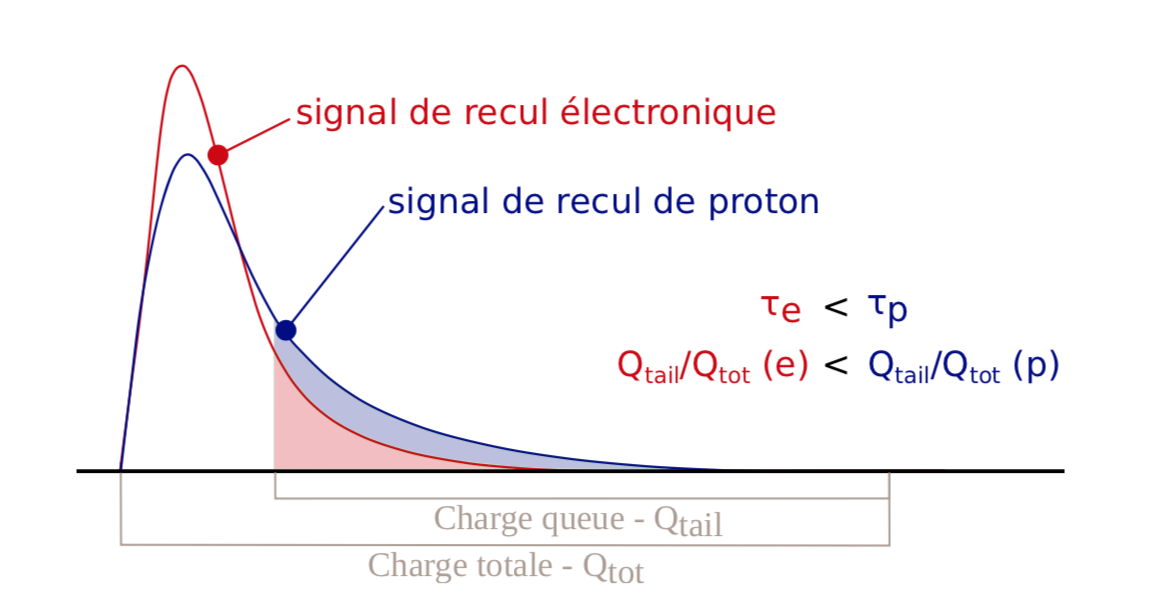
\includegraphics[width=1\textwidth]{images/Qtail_schem.png}
\caption[Principe de la discrimination par forme des signaux.]{Principe de la discrimination par forme des signaux. Les signaux induits par recul électronique (rouge) ont un rapport $Q_\textrm{tail}/Q_\textrm{tot}$ plus faible que ceux des protons de recul (bleu).}
\label{fig:Qtail_schem.png}
\end{figure}

}

Comme il a été décrit dans la section \ref{seq:scintillation}, les constantes de désexcitations différentes des molécules responsables du processus de scintillation permettent de distinguer les dépôts d'énergie par un électron de ceux d'un proton avec l'observable : $PSD \doteq Q_\textrm{tail}/Q_\textrm{tot}$. Les neutrons rapides sont détectés par leur interaction avec des protons du liquide scintillateur et sont attendus avec une haute PSD. En revanche, les positrons créés par les neutrinos déposent leur énergie par ionisation comme les électrons et ont donc une PSD plus faible. Le principe de discrimination est schématisé sur la figure \ref{fig:Qtail_schem.png}. La composante neutron des bruits de fond corrélés joue pour 80 \%, donc l'utilisation de la PSD offre une opportunité unique de réduire sa contribution drastiquement.\\

La forme des pulses de chaque événement n'étant pas enregistrée pendant la prise de données neutrino, seule les variables $Q_\textrm{tot}$ et $Q_\textrm{tail}$ calculées à la volée sont conservées. La qualité de la discrimination réside dans le choix de la borne d'intégration en temps de $Q_\textrm{tail}$ choisie en amont de la prise de données. L'optimisation de cette valeur a été effectuée en déployant la source d'AmBe. La performance de la séparation est quantifiée par le facteur de mérite défini tel que:

\begin{equation}
    F = \frac{\mu_e + \mu_p}{2.35 \times (\sigma_e + \sigma_p)},
\end{equation}

\bigbreak

où $\mu_e$ et $\mu_p$ sont les valeurs moyennes des distributions de PSD des électrons et des protons respectivement, et  $\sigma_e$ et $\sigma_p$ leur écart type. Concrètement, ce facteur mesure la distance en PSD des deux populations en unité de leur écart type. La borne d'intégration a été optimisée pour chaque cellule sur deux plages en énergie, $\sim \SI{1}{MeV_{ee}}$ et $\sim \SI{2.2}{MeV_{ee}}$\footnote{\og ee \fg{} signifie équivalent électron; le détecteur est calibré avec des gammas, qui déposent de l'énergie via les électrons qu'ils produisent, mais cette échelle en énergie n'est qu'arbitraire pour les neutrons.}, en ajustant deux gaussiennes pour reproduire la distribution de PSD. L'optimum a été atteint avec un facteur de mérite de 0,7 en phase 2 à $\SI{2,2}{MeVee}$ \cite{docdb409} contre 0,6 en phase 1 \cite{docdb155}.\\

L'évolution en temps et en énergie de $\mu_e$ et $\sigma_e$ nécessite une attention particulière pour suivre la position du signal neutrino sur la figure de PSD. En effet, la PSD est une observable qui dépend des effets de volume sur la collection de lumière, et l'augmentation progressive des fuites de lumière entre cellules pendant la prise de données a fait évoluer les paramètres $\mu_e$ et $\mu_p$ ainsi que leurs écart-types. De plus, les propriétés de scintillation du liquide sont sensibles à la température donc les moyennes $\mu_e$ et $\mu_p$ sont également corrélés avec la température du liquide.\\

Les événements Simples, principalement constitués de gammas, sont des candidats de choix pour suivre l'évolution en temps et en énergie de la PSD: $\mu_\gamma$ et $\sigma_\gamma$. Trois conditions sont imposées sur les événements Simples pour suivre la cellule $i$:

\begin{itemize}[label=\textbullet]
    \item Un événement Simple ne doit pas être étiqueté comme muon,
    \item Pas de corrélation avec un muon : $T(\textrm{Simple}) - T_\mu > \Delta T_\mu$,
    \item L'énergie reconstruite dans chaque cellule voisine ne doit pas excéder $\SI{0.7}{MeV}$.
\end{itemize}

\bigbreak

L'évolution en énergie est présentée sur la figure \ref{fig:PSD_gamma_vs_energy.png} et montre que $\mu_\gamma$ reste stable tandis que $\sigma_\gamma$ diminue de 30 \% avec l'énergie sur une échelle de 2 à $\SI{8}{MeV}$ grâce à l'évolution de la photostatistique. D'autre part, les évolutions en temps sont mesurées par échantillon d'une semaine. En phase 1, l'augmentation des fuites de lumière est la principale responsable des dérives de la PSD comme le montre la figure \ref{fig:PSD_vs_LL.png}. Entre mi-novembre 2016 et mi-décembre 2016, la PSD moyenne des événements Simples a chuté à hauteur d'environ 1 $\sigma_\gamma$. Les conditions de mesure en phase 2 étant plus stables, les variations de la PSD sont moindres et laissent apparaitre une anti-corrélation nette avec la température du liquide (voire figure \ref{fig:PSD_vs_temperature.png}). Il est important de noter que les montées de température coïncident avec les périodes de fonctionnement du réacteur. En effet, la soustraction des bruits de fond corrélés est basée sur la comparaison des distributions de PSD entre les périodes réacteur ON et OFF, donc cette évolution doit être prise en compte.\\

\afterpage{
%

\begin{figure}[h!]
\centering
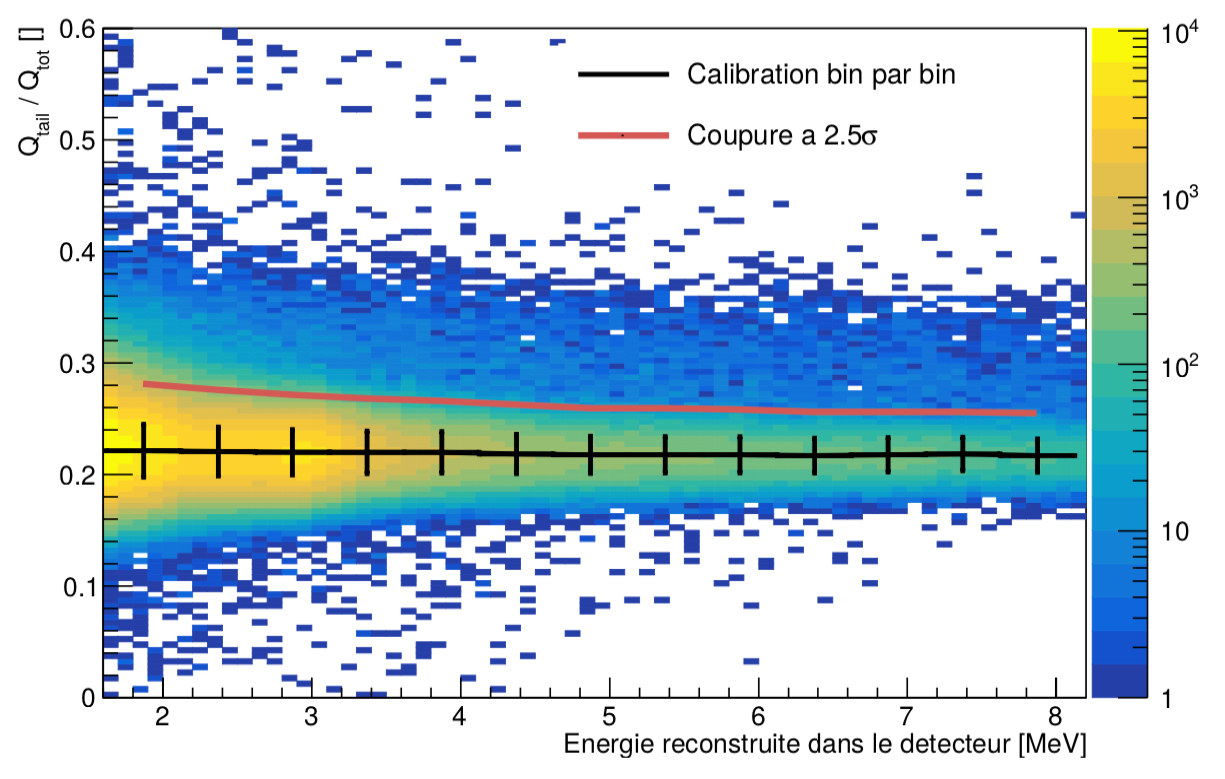
\includegraphics[width=0.8\textwidth]{images/PSD_gamma_vs_energy.png}
\caption[Évolution de la PSD des événements Simples avec l'énergie.]{Évolution de la PSD des événements Simples avec l'énergie. L'échantillon choisi provient de données acquises pendant une semaine en phase 1 qui sont des événements Simples identifiés dans la cellule 1. Les points en noir indiquent la position de $\mu_\gamma$ et la ligne rouge délimite à titre indicatif l'écart type correspondant à $2.5 \sigma_\gamma$.}
\label{fig:PSD_gamma_vs_energy.png}
\end{figure}

\begin{figure}[h!]
\centering
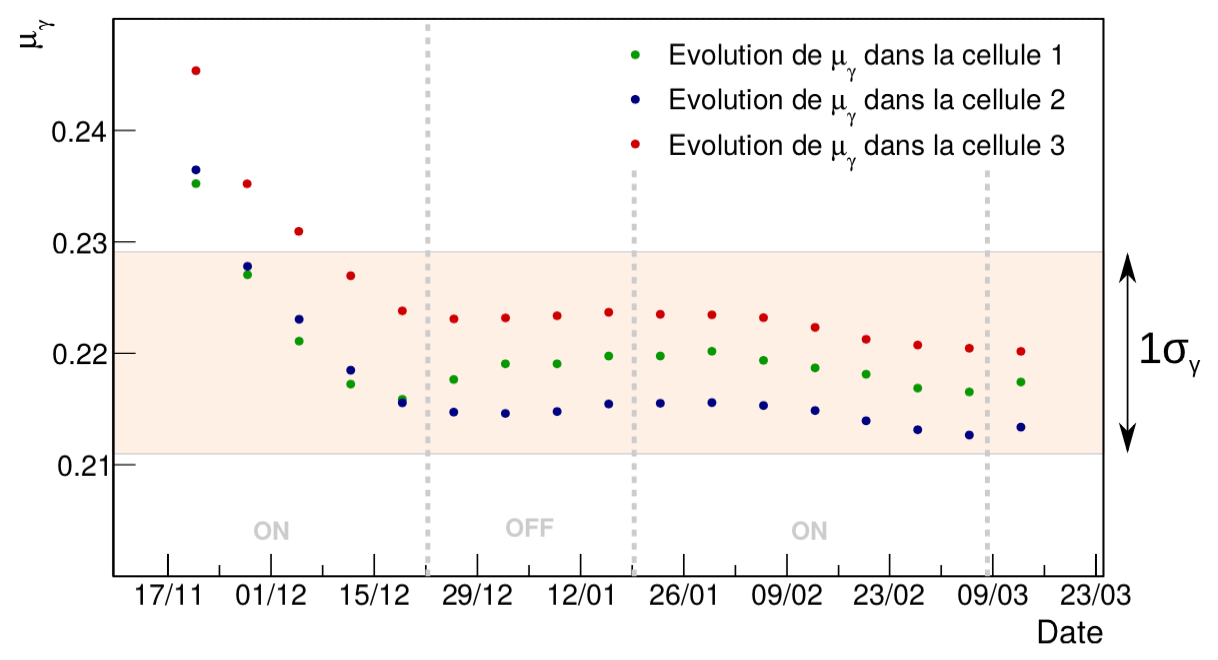
\includegraphics[width=0.8\textwidth]{images/PSD_vs_LL.png}
\caption[Évolution de la PSD dans le temps.]{Évolution pendant la phase 1 de la PSD moyenne $\mu_\gamma$ des événements Simples dans un intervalle en énergie de $\SI{500}{keV}$ centré sur $\SI{3.875}{MeV}$. Chaque point rassemble 1 semaine de prise de données. La dérive en début de période coïncide avec le développement des fuites de lumière dans le détecteur. L'amplitude de variation est à comparer avec la déviation standard des distributions de PSD ($\sigma_\gamma$) représenté par une bande colorée.}
\label{fig:PSD_vs_LL.png}
\end{figure}

\begin{figure}[h!]
\centering
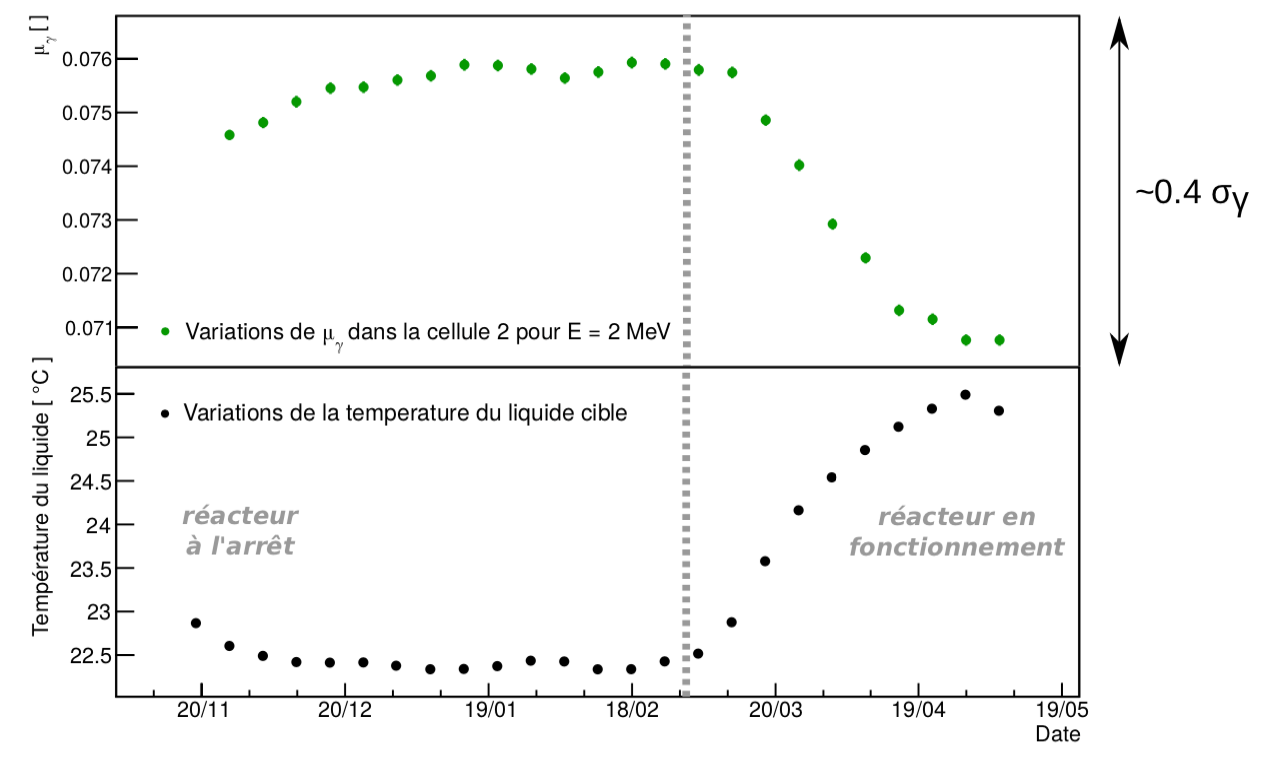
\includegraphics[width=0.9\textwidth]{images/PSD_vs_temperature.png}
\caption[Corrélation entre la PSD et la température du liquide.]{Corrélation entre la PSD moyenne $\mu_\gamma$ des événements Simples et la température du liquide pendant la phase 2. Les événements Simples sont choisis dans un intervalle de $\SI{500}{keV}$ centré sur $\SI{1.875}{MeV}$ et identifiés dans la cellule 2.}
\label{fig:PSD_vs_temperature.png}
\end{figure}

%\begin{figure}[h!]
%\centering
%\begin{subfigure}[b]{0.49\textwidth}
%
%\centering
%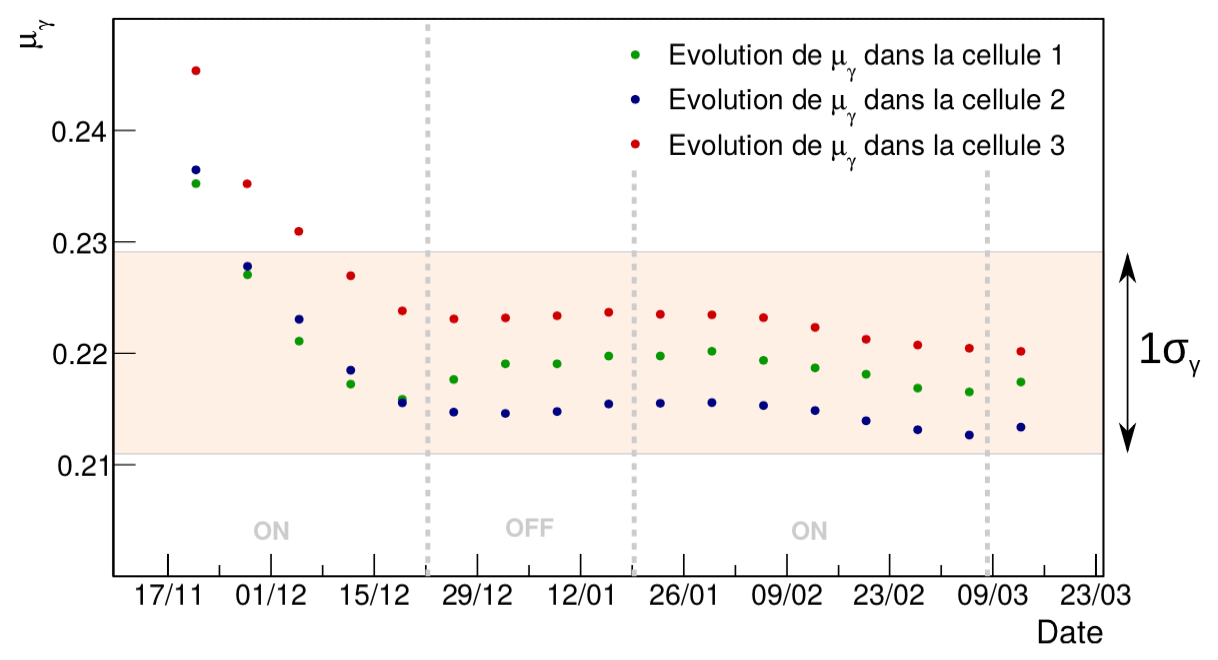
\includegraphics[width=1\textwidth]{images/PSD_vs_LL.png}
%\captionof{figure}{}
%\label{fig:PSD_vs_LL.png}
%
%\end{subfigure}
%~ % attention ! space sensitive
%\begin{subfigure}[b]{0.49\textwidth}
%
%\centering
%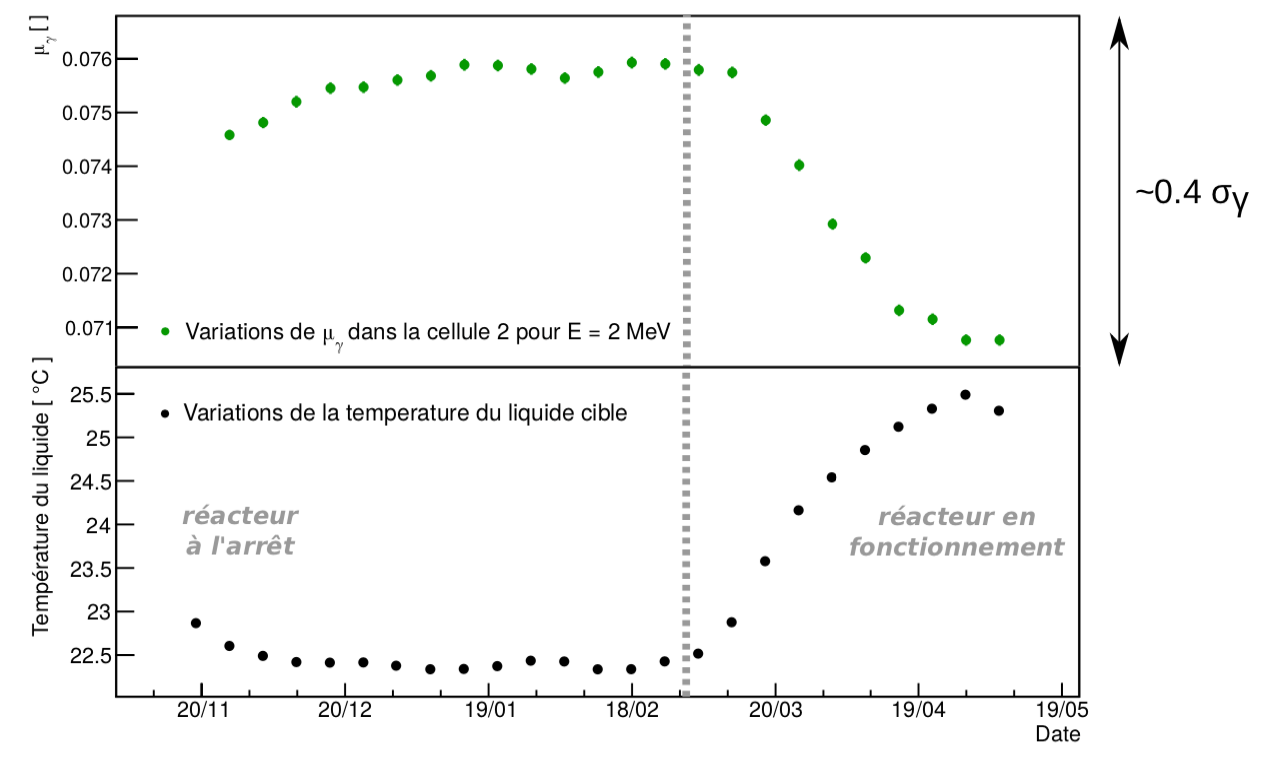
\includegraphics[width=1\textwidth]{images/PSD_vs_temperature.png}
%\captionof{figure}{}
%\label{fig:PSD_vs_temperature.png}
%
%\end{subfigure}
%%\captionof{figure}{Test}
%\caption{Test}
%\label{fig:PSD_vs_time}
%\end{figure}

\begin{figure}[h!]
\centering
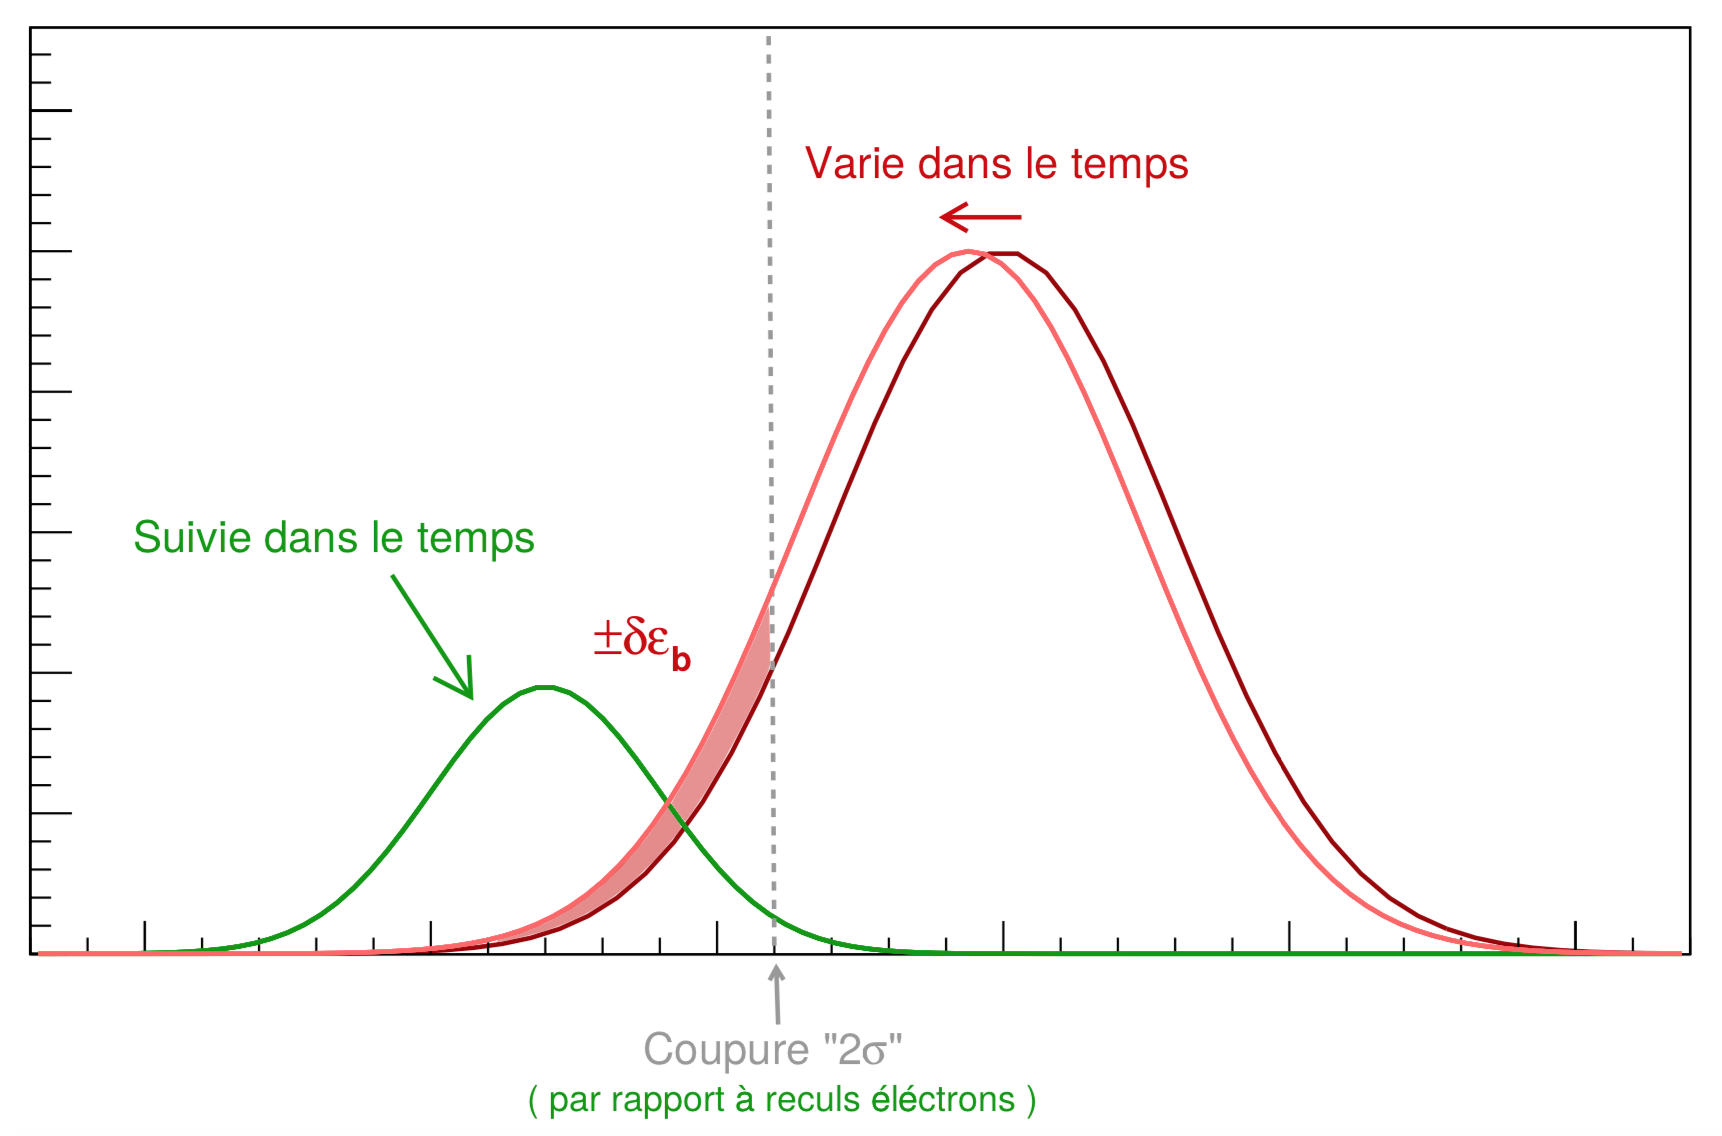
\includegraphics[width=0.8\textwidth]{images/no_cut_on_PSD.png}
\caption[Effet des variations relatives entre la PSD des reculs électroniques et la PSD des reculs de protons sur la procédure de soustraction.]{Effet des variations relatives entre la PSD des reculs électroniques et la PSD des reculs de protons sur la procédure de soustraction. Bien que la composante neutrino soit suivi dans le temps (vert), les variations relatives des protons de reculs entrainent un biais sur l'extraction du taux de comptages neutrino $\delta \varepsilon_b$.}
\label{fig:no_cut_on_PSD.png}
\end{figure}

\clearpage

}



%\begin{itemize}
%    \item Pourquoi pas de coupure stricte ?
%    \item Dépendance avec température
%    \item Correction JS
%\end{itemize}

\subsection{Extraction des taux de neutrinos dans chaque cellule et bin en énergie}
\label{sec:nu_extraction}

La reconstruction des spectres neutrino est accomplie en soustrayant le taux de  paires corrélées lorsque le réacteur est ON du taux obtenu lorsque le réacteur est OFF. Pour ce faire, les distributions de PSD sont isolées sur chaque plage en énergie reconstruite $\left[E, E+ \Delta E\right]$ et les figures de PSD en ON sont soustraites des distributions en OFF associées. L'intégrale des distributions soustraites fournit le nombre de neutrinos mesurés dans chaque bin en énergie.\\

L'utilisation d'une coupure sur la PSD s'avère nécessaire pour réduire l'incertitude sur la quantité de neutrinos extraite. Or, les variations de la PSD avec le temps rendent la tâche plus difficile à maitriser. Lorsqu'une coupure $\kappa$ sur la PSD est imposée telle que :

\begin{equation}
\label{eq:hard_PSD_cut}
    Q_\textrm{tail}/Q_\textrm{tot} < \mu_\gamma(t) + \kappa \sigma_\gamma(t),
\end{equation}

\bigbreak

le taux de neutrino extrait présente des variations résiduelles dépendantes de $\kappa$. La contamination de la composante des protons de recul est alors différente entre périodes ON et OFF, et la soustraction n'est donc plus valide. Ce phénomène est illustré sur la figure \ref{fig:no_cut_on_PSD.png}.\\

\subsubsection*{Méthode d'extraction des neutrinos par modélisation gaussienne des composantes PSD}
\label{sec:aurelie_nu_extraction}

Pour s'affranchir des évolutions du spectre PSD, un première méthode d'extraction des neutrinos a été développée. Celle-ci consiste à modéliser chaque composante de la figure de PSD par des fonctions gaussiennes. Les composantes du bruit de fond sont ajustées avec les données OFF :

\begin{equation}
    M_\textrm{OFF}(t, PSD) = \color{red}\mathcal{A}^{OFF}_p(t) \color{black} \left( \frac{\color{blue}\mathcal{A}^{OFF}_\gamma(t) \color{black}}{\color{red}\mathcal{A}^{OFF}_p(t)\color{black}}\color{blue} \mathcal{M}_\gamma(t, PSD) \color{black} + \color{red} \mathcal{M}_p(t, PSD)\color{black}\right),
\end{equation}

\bigbreak

avec les termes en rouge qui représentent la composante protons de recul du bruit de fond et en bleu les gammas. La forme des distributions est encodée dans les densités de probabilité (gaussiennes) notées $\mathcal{M}_i$, et $\mathcal{A}_i$ désigne l'intensité de chaque composante. Puisque la nature des bruits de fond corrélés est la même pendant les périodes ON, le rapport $\color{orange}\mathcal{A}_\gamma / \mathcal{A}_p\color{black}$ est une constante. Les données réacteur OFF mesurent donc cette valeur et elle seule est propagée dans le modèle de PSD réacteur ON:

\begin{equation}
    M_{ON}(t, PSD) = \color{red}\mathcal{A}^{ON}_p(t) \color{black} \left( \color{orange}\frac{\mathcal{A}_\gamma(t)}{\mathcal{A}_p(t)} \color{black} \color{blue} \mathcal{M}_\gamma(t, PSD) \color{black} + \color{red} \mathcal{M}_p(t, PSD)\color{black}\right) + \color{black!30!green} \mathcal{A}_\nu(t) \mathcal{M}_\nu(t, PSD) \color{black},
\end{equation}

\bigbreak

où $\color{black!30!green} \mathcal{A}_\nu \color{black}$ et $\color{black!30!green} \mathcal{M}_\nu \color{black}$ sont respectivement l'intensité et la forme du signal neutrino. La bosse proton étant toujours distincte de celle des neutrinos, son intensité, sa moyenne et son écart type restent ajustables en ON. La position et la largeur de la gaussienne gamma du bruit de fond sont eux connus par les accidentels, dominés par les gammas. Ainsi le bruit de fond $\gamma$ caché sous les neutrinos pendant les périodes ON est parfaitement contraint. Finalement, la valeur $\color{black!30!green}\mathcal{A}_\nu\color{black}$ ajustée donne le taux de neutrinos contribuant à la plage en énergie sélectionnée. Notons que contrairement à l'utilisation d'une coupure brute (Eq. \ref{eq:hard_PSD_cut}), cette procédure autorise les variations de $\mu_p$ entre les périodes ON et OFF. La seule hypothèse en jeu est la constance du rapport $\color{orange}\mathcal{A}_\gamma / \mathcal{A}_p\color{black}$.\\

La stabilité du rapport $\color{orange}\mathcal{A}_\gamma/\mathcal{A}_p \color{black}$ a été vérifiée sur l'ensemble de la phase 1 comme le montre la figure \ref{fig:Ag_Ap_stability.png}. Ensuite $M_{ON}$ est ajusté sur les données réacteur ON en fixant cette fois le rapport $\color{orange}\mathcal{A}_\gamma/\mathcal{A}_p \color{black}$ mesuré en OFF. Les paramètres de la gaussienne neutrino $\mathcal{M}_\nu$ sont ajustés et la valeur $\color{black!30!green}\mathcal{A}_\nu\color{black}$ obtenue donne le taux de neutrinos mesuré dans le bin en énergie $\left[E, E+\Delta E\right]$ d'une des 6 cellules.\\

Bien qu'a priori la composante gamma du bruit de fond corrélé soit de même nature que les accidentelles, des déviations significatives sont observées notamment entre 5 à $\SI{6}{MeV}$ en énergie reconstruite. En effet, dans cette région en énergie une partie des signaux Prompt associés aux bruits de fond proviennent de la diffusion de neutrons rapides sur le Carbone 12 : $\ce{^{12}C}(n, n^* \gamma)\ce{^{12}C}$. Ces événements sont donc le fruit d'un empilement d'énergies déposées à la fois par des gammas et par des neutrons, hybridant leur PSD. Pour tenir compte de cet effet, la déviation relative par rapport à $\mu_\textrm{gamma}$ est mesurée en OFF pour être propagée en ON.\\

Par ailleurs, la présence d'une épaule à haute PSD (supérieure à la moyenne proton) a été remarquée avec la statistique accrue de la phase 2. Plusieurs études ont été entreprises pour tenter d'identifier la nature de ces événements, mais aucune n'a pu la déduire. En revanche, cette nouvelle composante est prise en compte par l'ajout d'une nouvelle gaussienne proton à côté de l'originale et ses paramètres sont ajustés en OFF et en ON.\\

Les figures de PSD sont en définitive séparées par cellule, bin en énergie et bin en temps, donc la statistique traitée est relativement faible. Un formalisme de vraisemblance est utilisé pour adapter les modèles $M_{OFF}$ et $M_{ON}$ en considérant les erreurs statistiques suivant des lois de Poisson. Remarquons qu'en pratique, la composante accidentelle est ajoutée dans $M_{OFF}$ et $M_{ON}$, car l'utilisation des distributions de PSD déjà soustraites peuvent faire intervenir des taux de comptage négatifs, non interprétables avec la statistique de Poisson. Ses paramètres sont en revanche ajustés indépendamment, car sa figure de PSD des accidentelles est mesurée à l'aide de la méthode des portes décalées en temps (présentée dans la section \ref{seq:acc_subtraction}).\\

Finalement, la minimisation du logarithme de la vraisemblance permet d'ajuster les paramètres d'intérêt sur les figures de PSD réacteur OFF ou ON:

\begin{equation}
    - ln(\mathcal{L}_0) = - ln(\mathcal{L}_\textrm{acc}) - ln(\mathcal{L}_\textrm{corr+acc}),
\end{equation}

\bigbreak

où $ln(\mathcal{L}_\textrm{acc})$ est le logarithme de la vraisemblance du modèle des accidentels et $ln(\mathcal{L}_\textrm{corr+acc})$ le logarithme de la vraisemblance du modèle $M_{ON}$ ou $M_{OFF}$ incluant les accidentelles. Un exemple d'ajustement est disposé sur la figure \ref{fig:20180525_Fit_20180405_Cell1_Bin4.pdf}.\\

\afterpage{

\begin{figure}[h!]
\centering
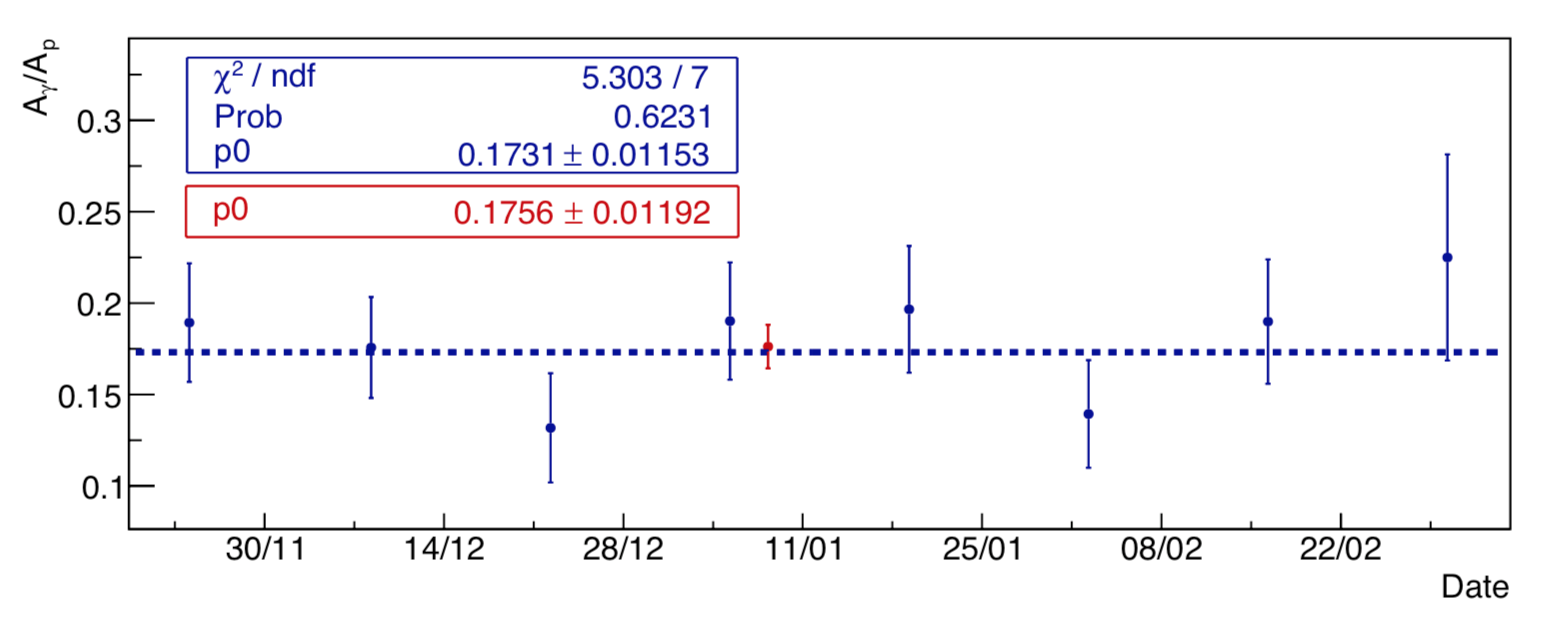
\includegraphics[width=0.8\textwidth]{images/Ag_Ap_stability.png}
\caption[Évolution du rapport $\mathcal{A}_\gamma/\mathcal{A}_p$ pendant la phase 1.]{Évolution du rapport $\mathcal{A}_\gamma/\mathcal{A}_p$ pendant la phase 1 pour la cellule 4 à $\SI{2.875}{MeV}$. Les points en bleu représentent des groupes de données de 14 jours alors que le point rouge est le résultat de l'ajustement du modèle avec toutes les données regroupées.}
\label{fig:Ag_Ap_stability.png}
\end{figure}

\begin{figure}[h!]
\centering
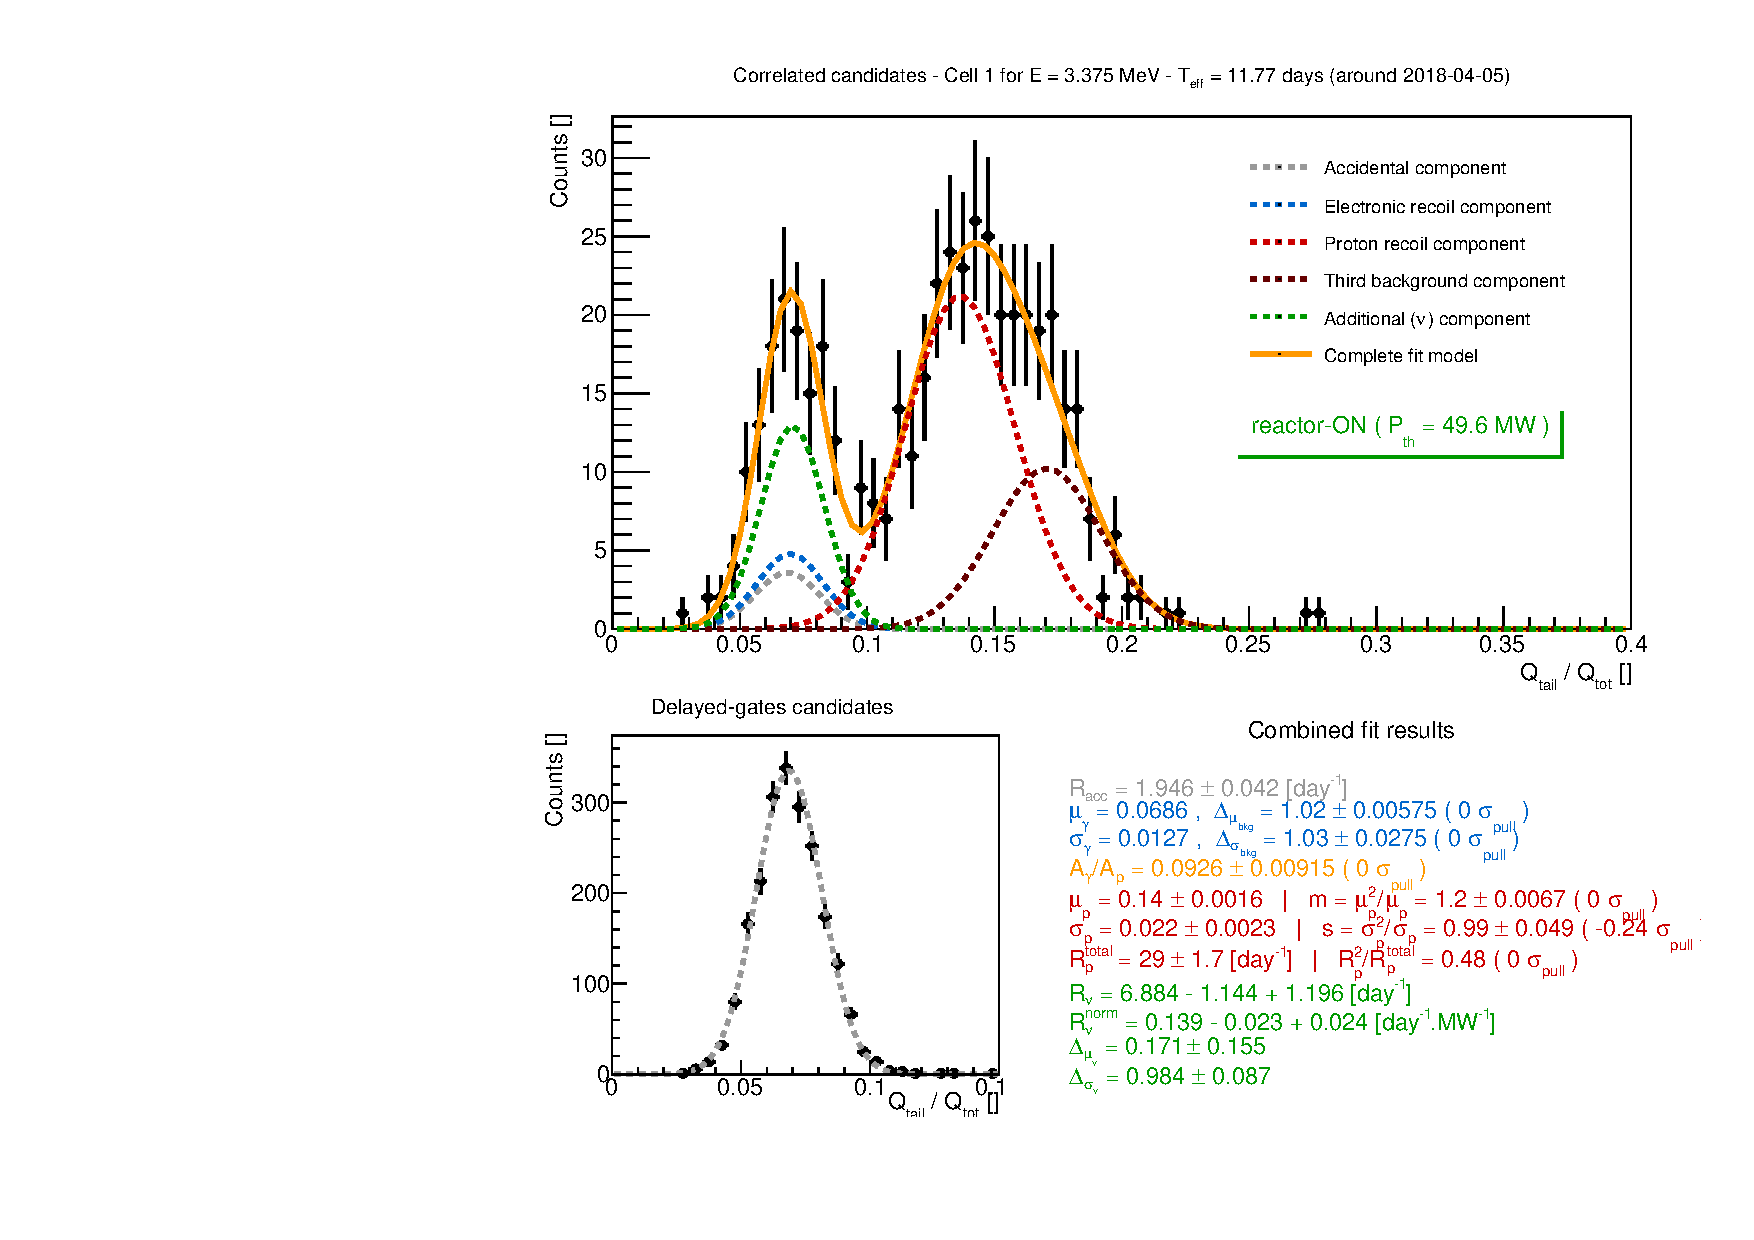
\includegraphics[width=0.8\textwidth]{images/20180525_Fit_20180405_Cell1_Bin4.pdf}
\caption[Exemple d'extraction du taux de candidats neutrinos par la méthode de modélisation gaussienne des composantes PSD]{Exemple d'extraction du taux de candidats neutrinos dans la cellule 1 et bin en énergie centré sur $\SI{3.375}{MeV}$, par la méthode de modélisation gaussienne des composantes PSD. L'ajustement du modèle (orange) est établi par les composantes : neutrino (vert), bruit de fond accidentel (gris), corrélé gamma (bleu), corrélé proton (rouge) et corrélé 2nd proton (bordeaux). Seul le paramètre $\mathcal{A}_\gamma / \mathcal{A}_p$ est propagé depuis l'ajustement sur les données OFF. (source : \cite{docdb665})}
\label{fig:20180525_Fit_20180405_Cell1_Bin4.pdf}
\end{figure}

}


%La procédure d'extraction de $\color{black!30!green}\mathcal{A}_\nu\color{black}$ se déroule dans un premier temps par la mesure du rapport $\color{orange}\mathcal{A}_\gamma/\mathcal{A}_p \color{black}$ en ajustant $M_{OFF}$ sur les données. Les paramètres de la gaussienne $\mathcal{M}_p$, $\mu_p$ et $\sigma_p$, ainsi que l'amplitude $\mathcal{A}_p$ sont ajustés librement sur la figure de PSD, alors que  la gaussienne $\mathcal{M}_\gamma$ est ajustée par rapport aux accidentelles: $\mu_\gamma/\mu_\textrm{acc}$ et $\sigma_\gamma/\sigma_\textrm{acc}$. Bien qu'a priori la composante gamma du bruit de fond corrélé soit de même nature que les accidentelles, des déviations significatives sont observées notamment entre 5 à $\SI{6}{MeV}$ en énergie reconstruite. En effet, dans cette région en énergie une partie des signaux Prompt associés aux bruits de fond proviennent de la diffusion de neutrons rapides sur le Carbone 12 : $\ce{^{12}C}(n, n^* \gamma)\ce{^{12}C}$. Ces événements sont donc le fruit d'un empilement d'énergies déposées à la fois par des gammas et par des neutrons, hybridant leur PSD. Cette effet est pris en compte dans la procédure de fit en autorisant $\mu_gamma$ à varier autour de $\mu_\textrm{acc}$.\\

% La stabilité du rapport $\color{orange}\mathcal{A}_\gamma/\mathcal{A}_p \color{black}$ a été vérifiée sur l'ensemble de la phase 1 comme le montre la figure \ref{fig:Ag_Ap_stability.png}. Ensuite $M_{ON}$ est ajusté sur les données réacteur ON en fixant cette fois le rapport $\color{orange}\mathcal{A}_\gamma/\mathcal{A}_p \color{black}$ mesurés en OFF. Les paramètres de la gaussienne neutrino $\mathcal{M}_\nu$ sont ajustés et la valeur $\color{black!30!green}\mathcal{A}_\nu\color{black}$ obtenue donne le taux de neutrinos mesuré dans le bin en énergie $\left[E, E+\Delta E\right]$ d'une des 6 cellules.\\

Avec cette méthode, la forme des densités de probabilités de chaque composante $\mathcal{M}_i$ a été approximée avec un modèle gaussien. L'évolution des moyennes $\mu_p$ et $\mu_e$ avec le temps contraint la procédure d'extraction à n'être appliquée que sur des plages en temps réduits $\left[T, T+\Delta T\right]$ pour s'assurer de la validité de la modélisation. Par ailleurs, les effets de volume sur la collection de lumière dispersent les temps d'arrivée des photons sur les PMs, et élargissent par cet effet les gaussiennes de PSD. Des études complémentaires ont été menées dans le cadre de cette thèse pour estimer les erreurs systématiques induites par l'utilisation de modèles gaussiens. Cette tâche a été effectuée en introduisant des modèles dits par \og \textit{templates} \fg{}, tenant compte des effets haut-bas sur la PSD. Ces derniers sont construits en tirant la PSD de chaque événement dans une gaussienne dont la moyenne $\mu_i$ et la largeur $\sigma_i$ sont choisies en amont suivant une densité de probabilité. La forme de ces densités de probabilité est générée en établissant la correspondance entre la hauteur Z dans le volume et les paramètres associés $\mu(Z)$ et $\sigma(Z)$. Les évolutions de $\mu(Z)$ et $\sigma(Z)$ ont été mesurées à l'aide de sources de calibration gamma. Un exemple d'échantillonnage de $\mu_\gamma(Z)$ avec la source de $\ce{^{54}Mn}$ est présenté sur la figure \ref{fig:Mean_Graph_PSD_vs_Z.pdf}. Un \textit{template} est généré suivant la procédure suivante:\\

\afterpage{

%

\begin{figure}[h!]
\centering
%\begin{minipage}[c]{.49\linewidth}
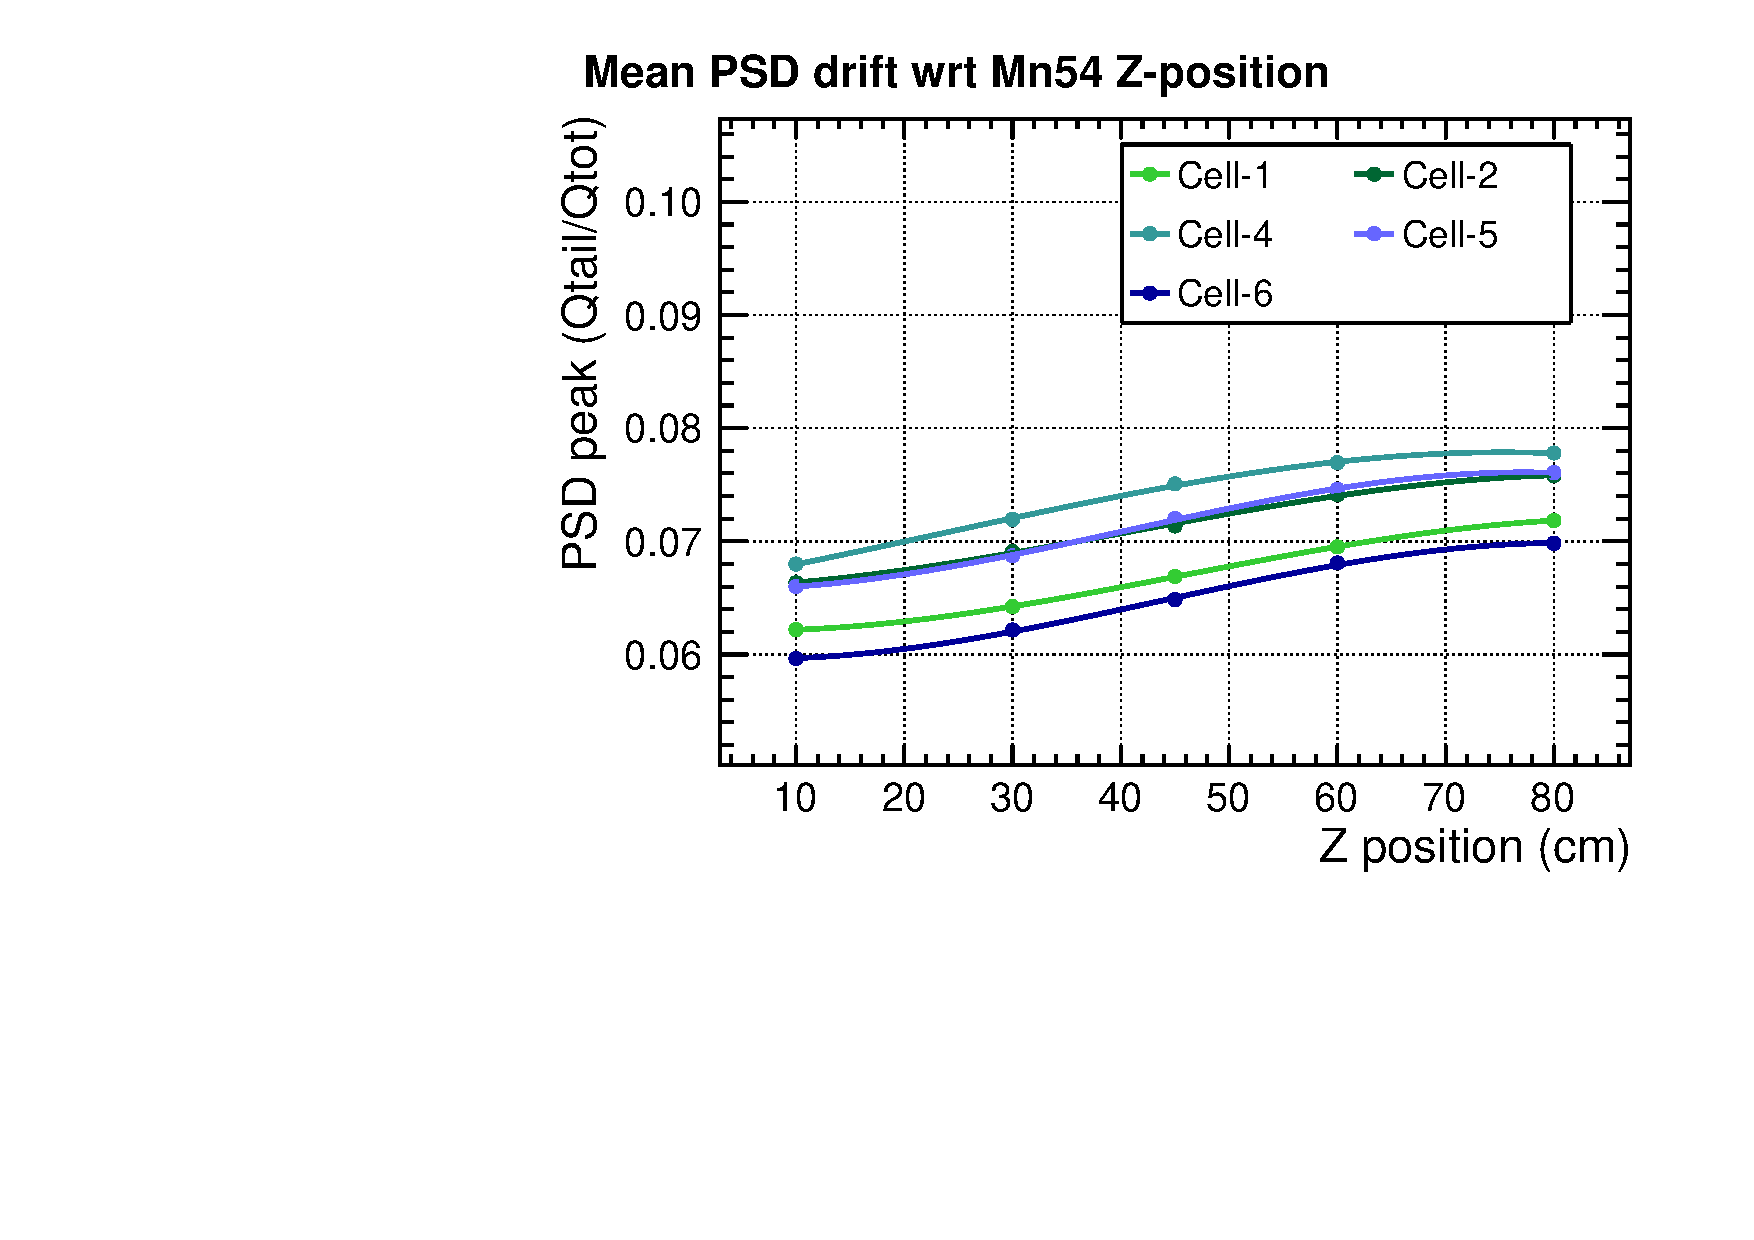
\includegraphics[width=0.8\textwidth]{images/Mean_Graph_PSD_vs_Z.pdf}
\caption[Evolution de la PSD moyenne en fonction de la hauteur]{Evolution de la PSD moyenne en fonction de la hauteur mesurée avec les runs source du $\ce{^{54}Mn}$. Ces distributions ont été exploitées en vue d'améliorer les modèles gaussiens utilisés dans l'extraction des taux de comptage neutrino.}
\label{fig:Mean_Graph_PSD_vs_Z.pdf}
%\end{minipage} \hfill
%\begin{minipage}[c]{.49\linewidth}
%    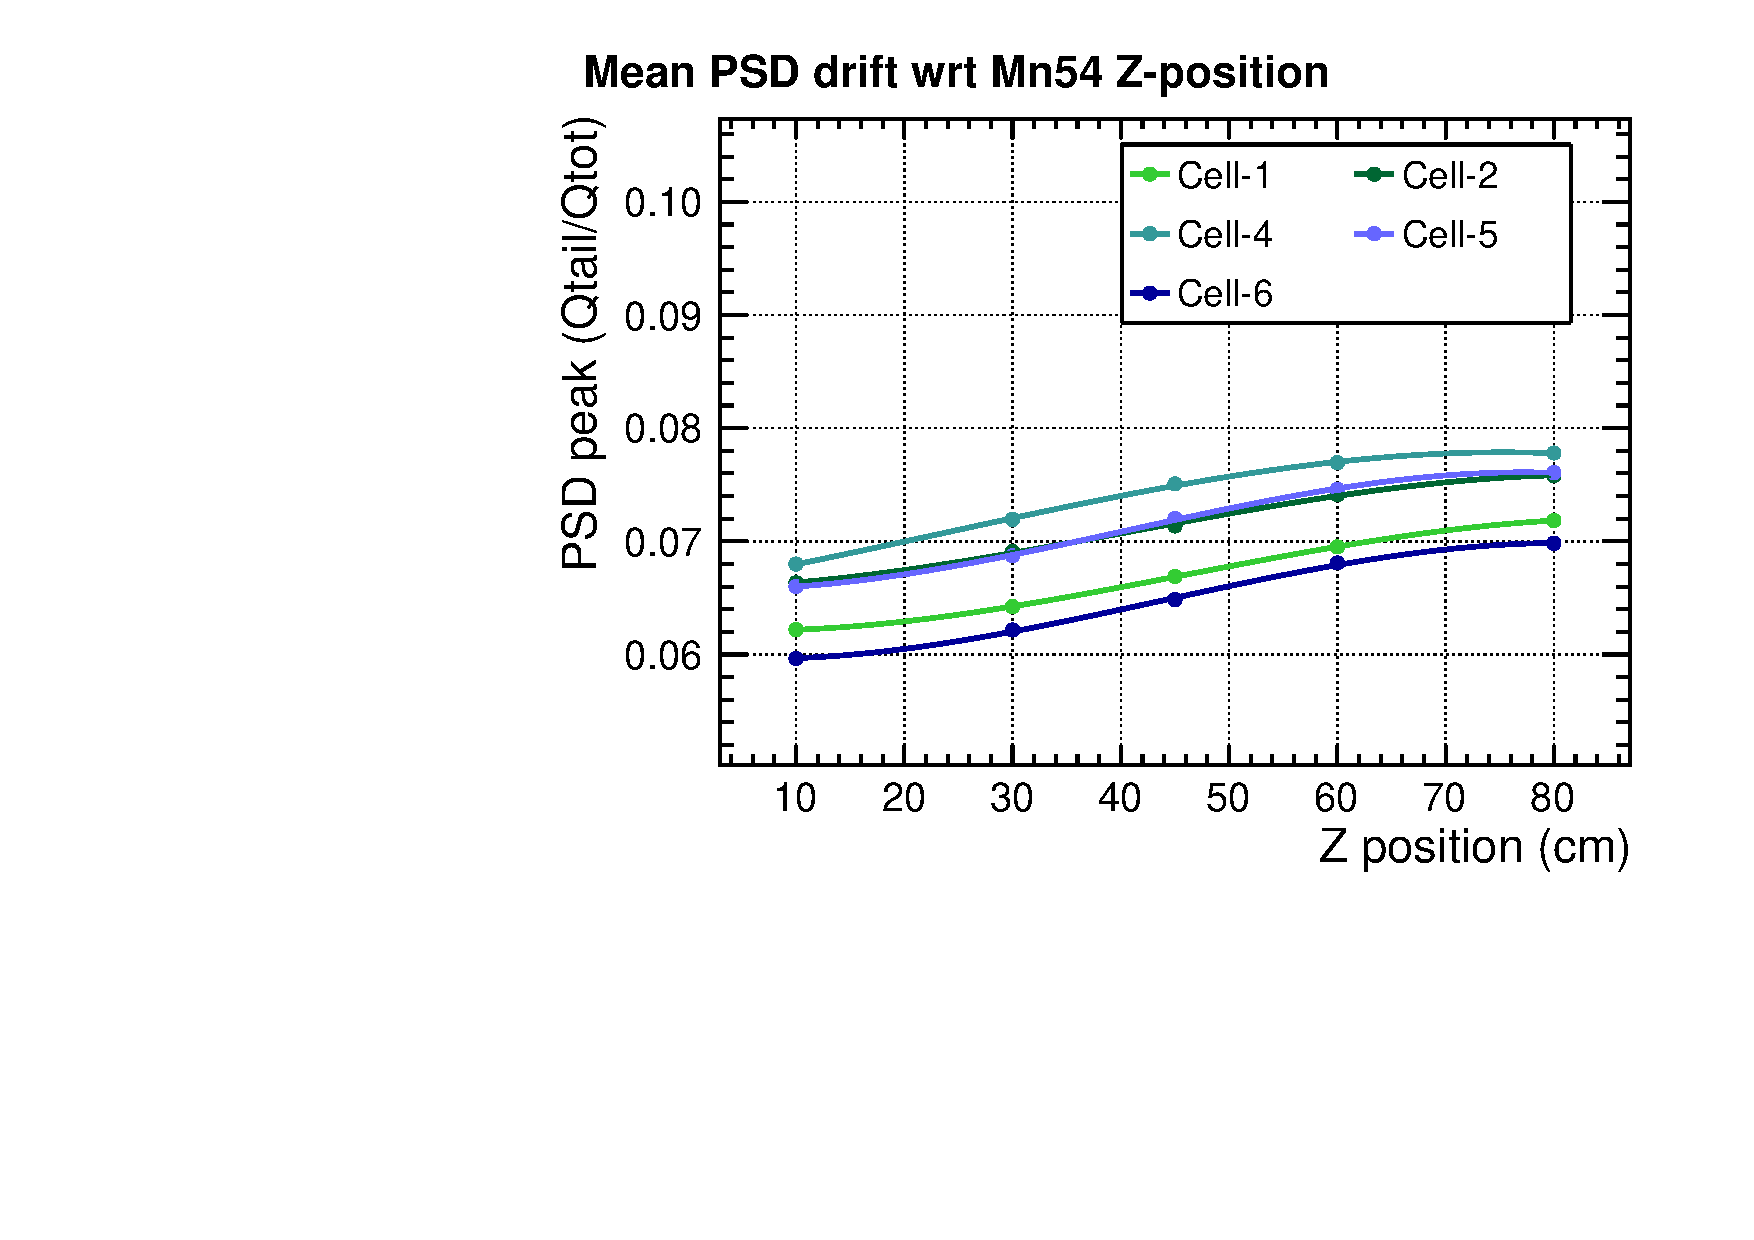
\includegraphics[width=0.9\textwidth]{images/Mean_Graph_PSD_vs_Z.pdf}
%\caption[Evolution de la PSD moyenne en fonction de la hauteur]{Evolution de la PSD moyenne en fonction de la hauteur mesuré avec les runs source du $\ce{^{54}Mn}$. Ces distributions ont été exploitées en vue d'améliorer les modèles gaussiens utilisés dans l'extraction des taux de comptage neutrino.}
%\label{fig:Mean_Graph_PSD_vs_Z.pdf}
%\end{minipage}



\end{figure}

}

\begin{itemize}[label=$\bullet$]
    \item (0) Une distribution d'événements en Z est choisie \textit{a priori} : par exemple homogène en Z pour les neutrinos, ou piqué au fond du détecteur pour les neutrons rapides,
    \item (1) Une valeur de Z est tirée aléatoirement suivant la densité de probabilité considérée,
    \item (2) Les paramètres de la gaussienne en PSD $\mu(Z)$ et $\sigma(Z)$ sont déduits,
    \item (3) Une valeur de PSD est tirée aléatoirement selon la gaussienne paramétrée par $\mu(Z)$ et $\sigma(Z)$,
    \item (4) La procédure est répétée depuis (1) pour remplir un histogramme formant le \textit{template} PSD associé à la distribution de vertex choisie \textit{a priori}.
\end{itemize}

\bigbreak

En comparant l'intégrale des deux modèles, gaussien et \textit{template}, ajustés sur une distribution de PSD mesurée avec une source gamma sur 5 hauteurs en Z, l'amplitude des erreurs systématiques est bornée entre: $0,1\% < \delta R/R = |R_\textrm{gaus} - R_\textrm{temp}|/R_\textrm{gaus} < 0,5\%$ \cite{docdb642}.\\

Par ailleurs, les variations de température et de fuites de lumière avec le temps élargissent aussi les distributions de PSD. Cependant, les biais induits par l'utilisation de gaussiennes pour extraire $\color{orange}\mathcal{A}_\gamma/\mathcal{A}_p\color{black}$ ne sont significatifs qu'à partir d'une dérive de la moyenne $\mu_\gamma$ d'amplitude supérieure à 2 $\sigma$ \cite{docdb717}, soit plus de 6 fois l'amplitude les dérives réellement observées. Les incertitudes systématiques liées à la modélisation par des gaussiennes sont en définitive négligées.\\

\subsubsection*{Correction des effets de dérives de la PSD}

\afterpage{

%
\begin{figure}[h!]
\centering
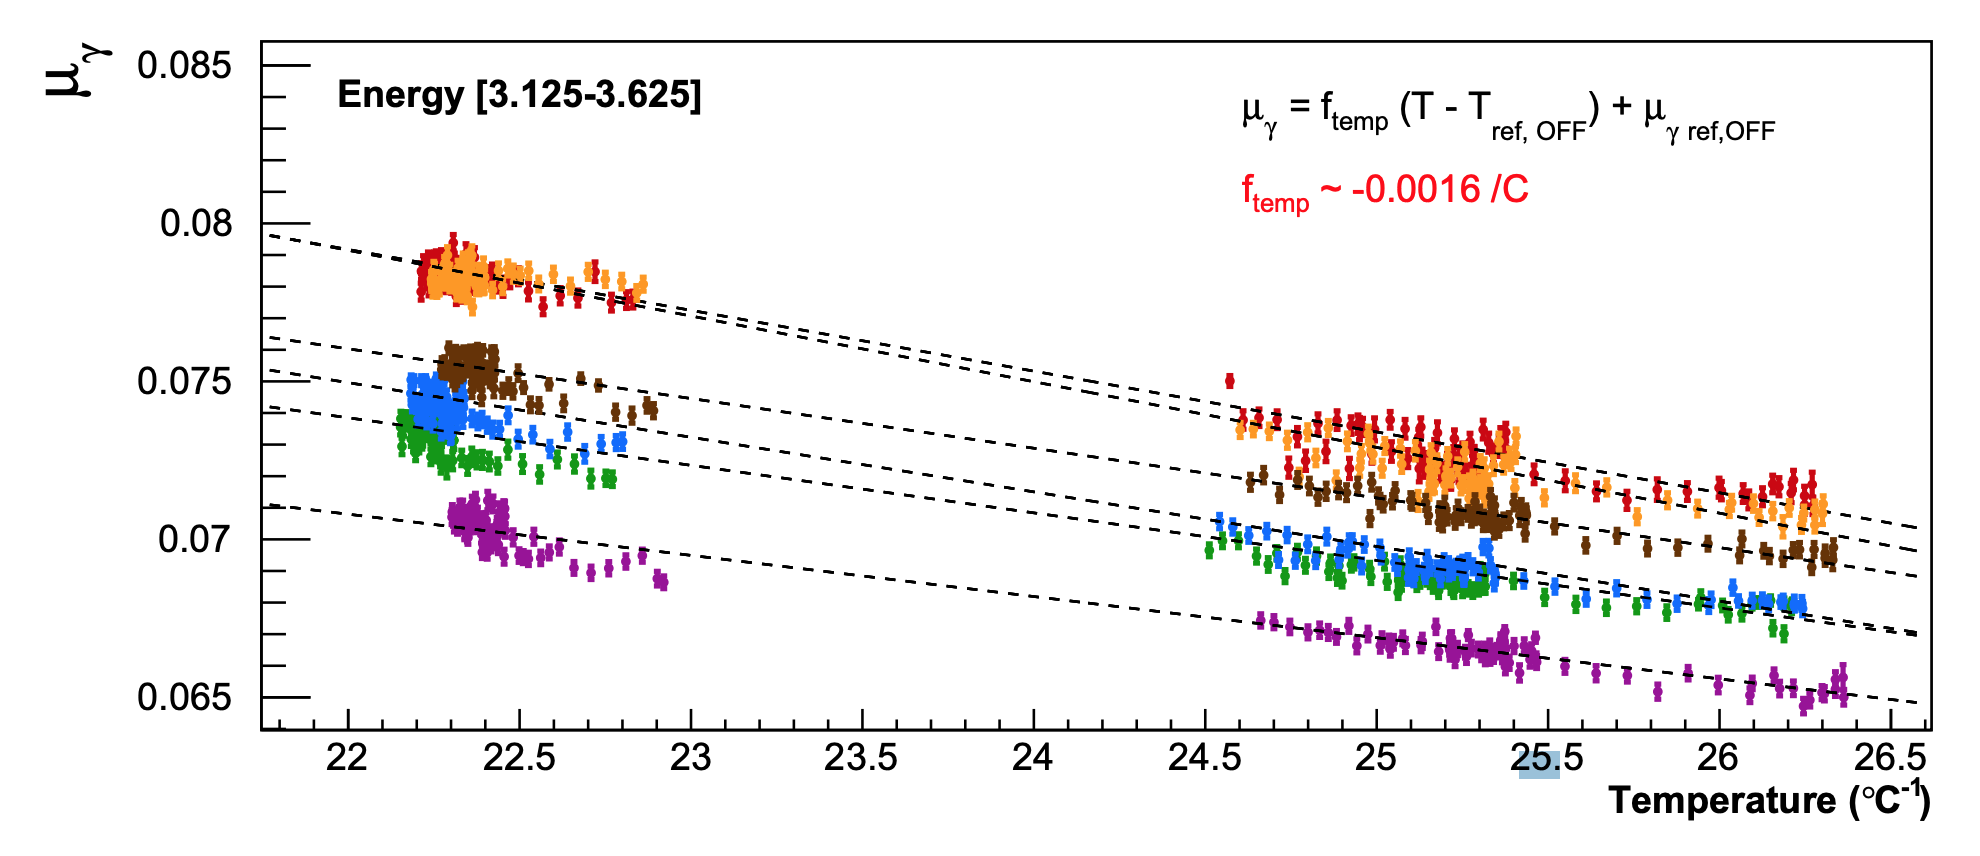
\includegraphics[width=0.8\textwidth]{images/PSD_vs_temp.png}
\caption[Corrélation de la PSD avec la température.]{Corrélation de la PSD avec la température. Les données utilisées sont issues des périodes OFF en phase 2. Le bin en énergie considéré ici est $[3.125-3.625]$ MeV, et chaque couleur correspond à une cellule. (source : \cite{docdb722})}
\label{fig:PSD_vs_temp.png}
\end{figure}

}

Les conditions d'acquisition étant plus stables pendant la seconde phase de prise de données, une correction de la PSD run à run a pu être utilisée. La principale cause des variations résiduelles de la PSD en phase 2 est la température. Ces variations sont corrigées en mesurant le coefficient de corrélation entre la PSD moyenne des événements Simples $\mu_\gamma$ et la température (voir figure \ref{fig:PSD_vs_temp.png}). À chaque run, le biais moyen $\delta PSD$ est calculé en fonction de la température :

\begin{equation}
    \delta PSD = (T_\textrm{ref} - T_\textrm{run}) f_\textrm{temp},
\end{equation}

\bigbreak

où $f_\textrm{temp}$ est le coefficient de corrélation et $T_\textrm{ref}$ est une température de référence choisie arbitrairement et commune à tous les runs. En appliquant ce décalage à chaque événement, $PSD^* = PSD + \delta PSD$, les dérives sont corrigées au premier ordre. Cependant la PSD des périodes ON et OFF ne présente pas les mêmes corrélations avec la température et des dérives temporelles subsistent, notamment en phase 1 à cause du développement des fuites de lumière. Pour régulariser ces biais résiduels, $\delta PSD$ est calculé itérativement, en mesurant la corrélation avec la température puis avec le temps à tour de rôle, jusqu'à ce que sa valeur converge, soit après une quinzaine d'itérations tout au plus \cite{docdb735}. Des études complémentaires avec la source d'AmBe ont montré que la correction de PSD exécutée sur les événements simples $\mu_\gamma$ se propage de la même manière sur la composante protons de recul $\mu_p$ \cite{docdb761}.\\

\subsubsection*{Méthode d'extraction des neutrinos par soustraction directe du bruit de fond}
\label{sec:laura_nu_extraction}

Cette procédure de décorrélation de la PSD a non seulement permis de s'affranchir de la segmentation en temps des données dans la première méthode d'extraction du signal neutrino, mais elle a aussi permis le développement d'une nouvelle méthode d'extraction exploitant directement la forme en PSD du bruit de fond mesuré pendant les périodes OFF. Les ingrédients de cette méthode se composent de :

\begin{itemize}[label=\textbullet]
    \item La PSD recalée des candidats corrélés + accidentels pendant les périodes réacteur ON: $\color{blue} ON \color{black}$,
    \item La PSD recalée des candidats corrélés + accidentels pendant les périodes réacteur OFF: $\color{red} OFF \color{black}$,
    \item La figure de PSD recalée des paires accidentelles mesurées avec la méthode des portes décalées pendant la période ON: $\color{darkgray} ON^\textrm{acc} \color{black}$,
    \item La figure de PSD recalée des paires accidentelles mesurées avec la méthode des portes décalées pendant la période OFF: $\color{darkgray} OFF^\textrm{acc} \color{black}$,
    \item Une gaussienne représentant la figure de PSD recalée des neutrinos: $\color{black!30!green} \mathcal{M}^\nu \color{black}$.
\end{itemize}

\bigbreak

\afterpage{

% FitPressure_relative.pdf
\begin{figure}[h!]
\centering
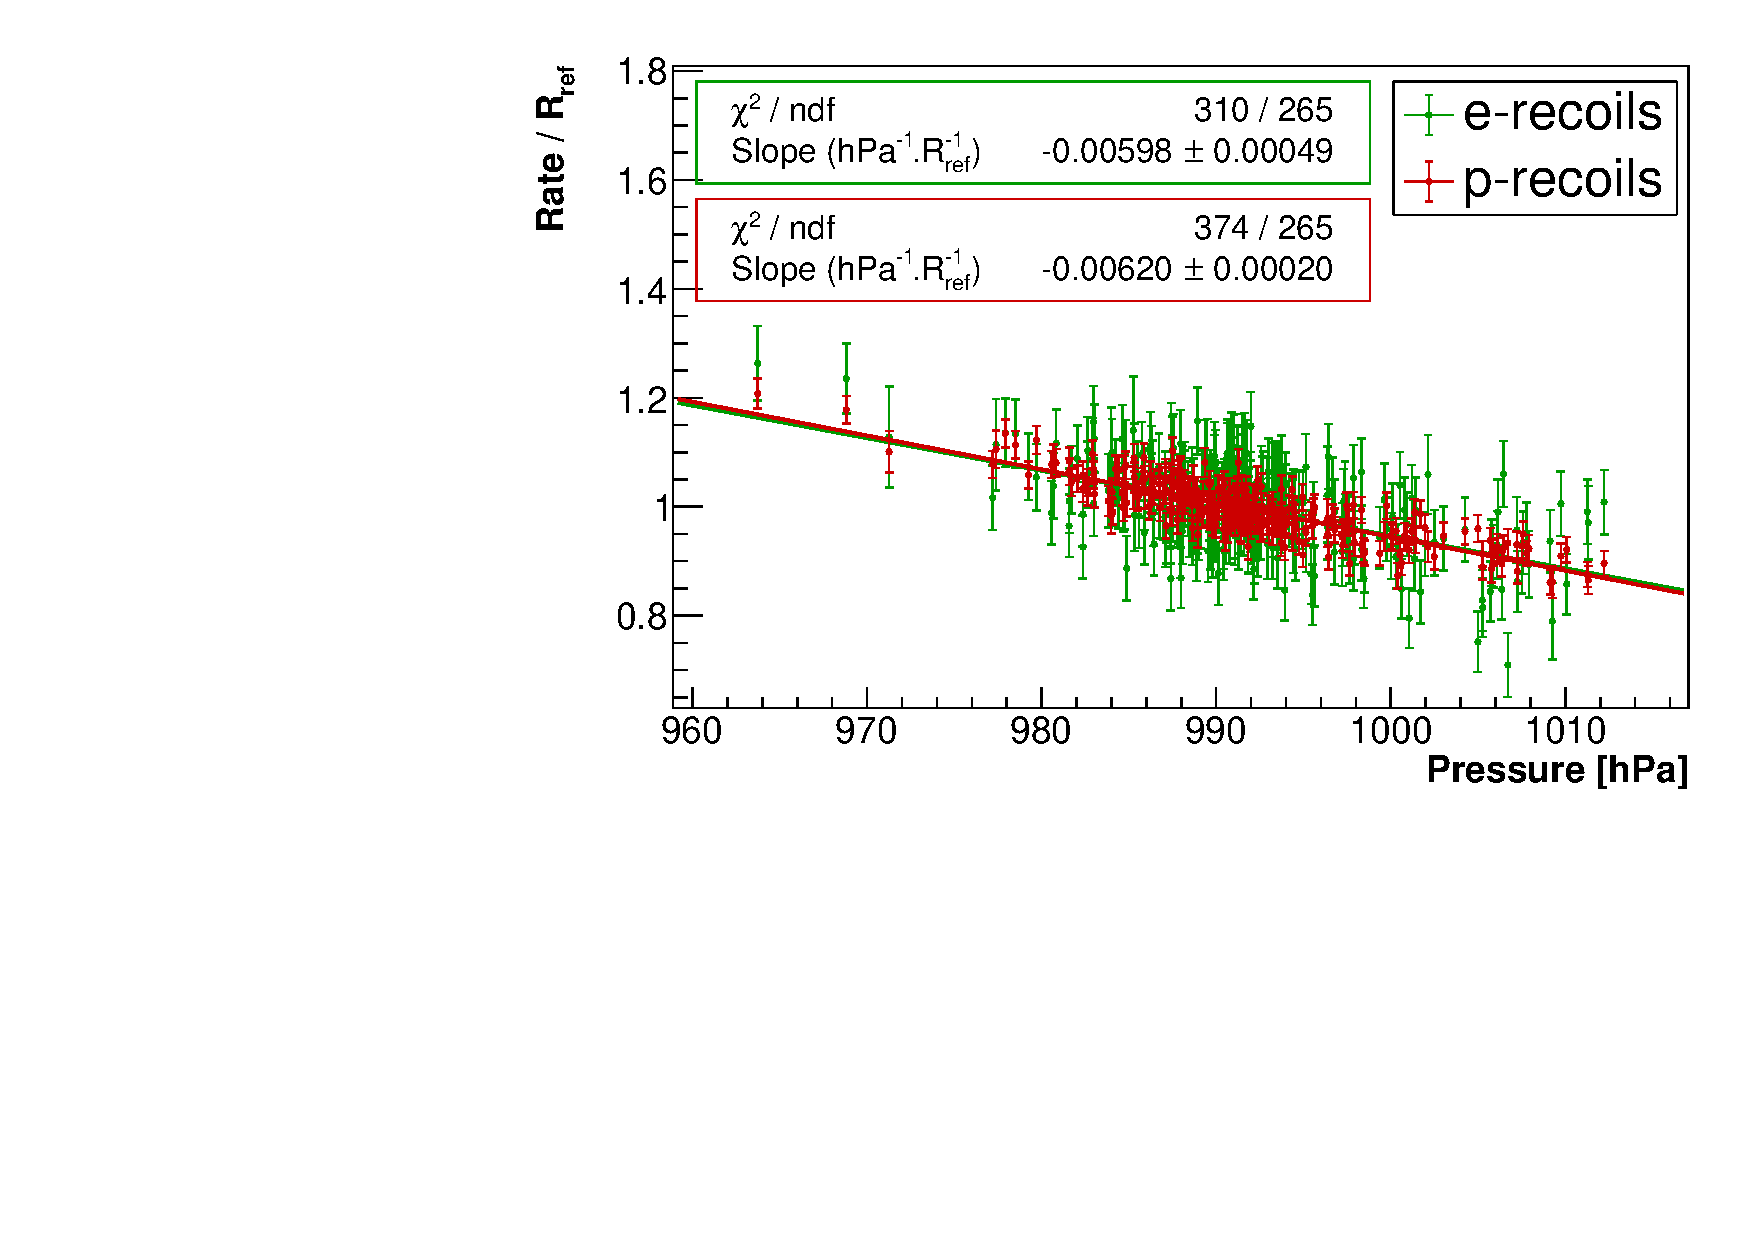
\includegraphics[width=0.7\textwidth]{images/FitPressure_relative.pdf}
\caption[Corrélation entre la pression atmosphérique et le taux de paires corrélées]{Corrélation entre la pression atmosphérique et le taux de paires corrélées pendant les périodes réacteur OFF. En vert est représentée la composante électrons de recul ($PSD < \mu_\gamma + 2\sigma_\gamma$) et en rouge les protons de reculs ($PSD > \mu_\gamma + 2\sigma_\gamma$). Les taux de contages ont été renormalisés par une valeur de référence $R_{ref}$ (une pour les électrons et une pour les protons) correspondante à la moyenne sur toute la période.}
\label{fig:FitPressure_relative.pdf}
\end{figure}

}

Le principe de cette méthode consiste à ajuster un modèle décrivant la figure de PSD $\color{blue} ON \color{black}$ à l'aide des contraintes offertes par $\color{red} OFF \color{black}$, $\color{darkgray} ON^\textrm{acc} \color{black}$, $\color{darkgray} OFF^\textrm{acc} \color{black}$. Chaque composante est autorisée de varier dans ses barres d'erreurs statistiques, et les contraintes sont formalisées avec des termes de traction (\og\textit{pull-terms}\fg{}).


% Le $\chi^2$ à minimiser a donc la forme suivante:

%\begin{align}
%    \chi^2 = \sum_i^\textrm{PSD bin}\left(\frac{\color{blue} ON_i \color{black} - \color{blue} \mathcal{M}_i^{ON} \color{black} (\color{red} \mathcal{M}_i^{OFF}\color{black}, \color{darkgray} \mathcal{M}_i^{OFF^\textrm{acc}} \color{black}, \color{darkgray} \mathcal{M}_i^{ON^\textrm{acc}} \color{black}, \color{black!30!green} \mathcal{M}^\nu_i \color{black})} {\color{blue}\sigma_i^\textrm{ON} \color{black}}\right)^2 \\
%    +  \left(\frac{\color{red} OFF_i \color{black} - \color{red} \mathcal{M}_i^{OFF} \color{black}(\color{darkgray} \mathcal{M}_i^{OFF^\textrm{acc}} \color{black})}{\color{red}\sigma_i^\textrm{OFF}\color{black}}\right)^2 \\
%    + \left(\frac{\color{darkgray} OFF_i^\textrm{acc} \color{black} - \color{darkgray} \mathcal{M}_i^{OFF^\textrm{acc}} \color{black}}{ \color{darkgray} \sigma_i^{OFF^\textrm{acc}} \color{black} }\right)^2\\
%    + \left(\frac{\color{darkgray} ON_i^\textrm{acc} \color{black} - \color{darkgray} \mathcal{M}_i^{ON^\textrm{acc}} \color{black}}{ \color{darkgray} \sigma_i^{ON^\textrm{acc}} \color{black} }\right)^2,
%\end{align}

\bigbreak

Dans le cas des accidentelles les modèles sont simplement des paramètres libres notés $\color{darkgray}m_i^{ON^\textrm{acc}}\color{black}$ et $\color{darkgray}m_i^{OFF^\textrm{acc}}\color{black}$. Le modèle OFF est constitué d'un paramètre libre représentant le bruit de fond corrélé et de $\color{darkgray}m_i^{OFF^\textrm{acc}}\color{black}$ : $\color{red}\mathcal{M}_i^{OFF} \color{black} \doteq \color{red}m_i^{OFF}\color{black} + \color{darkgray}m_i^{OFF^\textrm{acc}}\color{black}$. Enfin le modèle ON $\color{blue}\mathcal{M}_i^{ON} \color{black}$ contient à la fois le bruit de fond corrélé $\color{red} m_i^{OFF}\color{black}$, les accidentelles en ON $\color{darkgray}m_i^{ON^\textrm{acc}}\color{black}$ et la gaussienne neutrino $\color{black!30!green} \mathcal{M}^\nu_i \color{black} \doteq \color{black!30!green}A_\nu g_i(\mu_\nu, \sigma_\nu)\color{black}$ où $g_i$ est une gaussienne normalisée et $A_\nu$ le taux de comptage neutrino.\\

Puisque le bruit de fond corrélé est principalement constitué d'événements cosmogéniques, leur flux varie en fonction de la pression atmosphérique. La corrélation entre le taux de bruits de fond corrélés et la pression atmosphérique est présentée sur la figure \ref{fig:FitPressure_relative.pdf}. Afin de prendre en compte cet effet, un facteur de normalisation $\color{orange} a \color{black}$ est ajouté dans l'expression du modèle de PSD ON: $\color{blue}\mathcal{M}_i^{ON} \color{black} = \color{orange} a \color{black}\color{red} m_i^{OFF}\color{black} + \color{darkgray}m_i^{ON^\textrm{acc}}\color{black} + \color{black!30!green}A_\nu g_i(\mu_\nu, \sigma_\nu)\color{black}$. Ainsi les paramètres $\color{darkgray}m_i^{ON^\textrm{acc}}\color{black}$, $\color{darkgray}m_i^{OFF^\textrm{acc}}\color{black}$, $\color{red} m_i^{OFF}\color{black}$, $\color{orange} a \color{black}$, $\color{black!30!green}\mu_\nu\color{black}$, $\color{black!30!green}\sigma_\nu\color{black}$ et $\color{black!30!green}A_\nu\color{black}$ sont ajustés en minimisant le $\chi^2$ suivant:

\begin{align}
        \chi^2 = \sum_i^\textrm{PSD bin}\left(\frac{\color{blue} ON_i \color{black} - (\color{orange} a \color{red} m_i^{OFF}\color{black} + \color{darkgray}m_i^{ON^\textrm{acc}}\color{black} + \color{black!30!green}A_\nu g_i(\mu_\nu, \sigma_\nu)\color{black})} {\color{blue}\sigma_i^\textrm{ON} \color{black}}\right)^2 \\
    +  \left(\frac{\color{red} OFF_i \color{black} - (\color{red} m_i^{OFF} \color{black} + \color{darkgray}m_i^{OFF^\textrm{acc}}\color{black})}{\color{red}\sigma_i^\textrm{OFF}\color{black}}\right)^2 \\
    + \left(\frac{\color{darkgray} OFF_i^\textrm{acc} \color{black} - \color{darkgray}m_i^{OFF^\textrm{acc}}\color{black}}{ \color{darkgray} \sigma_i^{OFF^\textrm{acc}} \color{black} }\right)^2\\
    + \left(\frac{\color{darkgray} ON_i^\textrm{acc} \color{black} - \color{darkgray}m_i^{ON^\textrm{acc}}\color{black}}{ \color{darkgray} \sigma_i^{ON^\textrm{acc}} \color{black} }\right)^2.
\end{align}

\bigbreak

\afterpage{

\begin{figure}[h!]
\centering
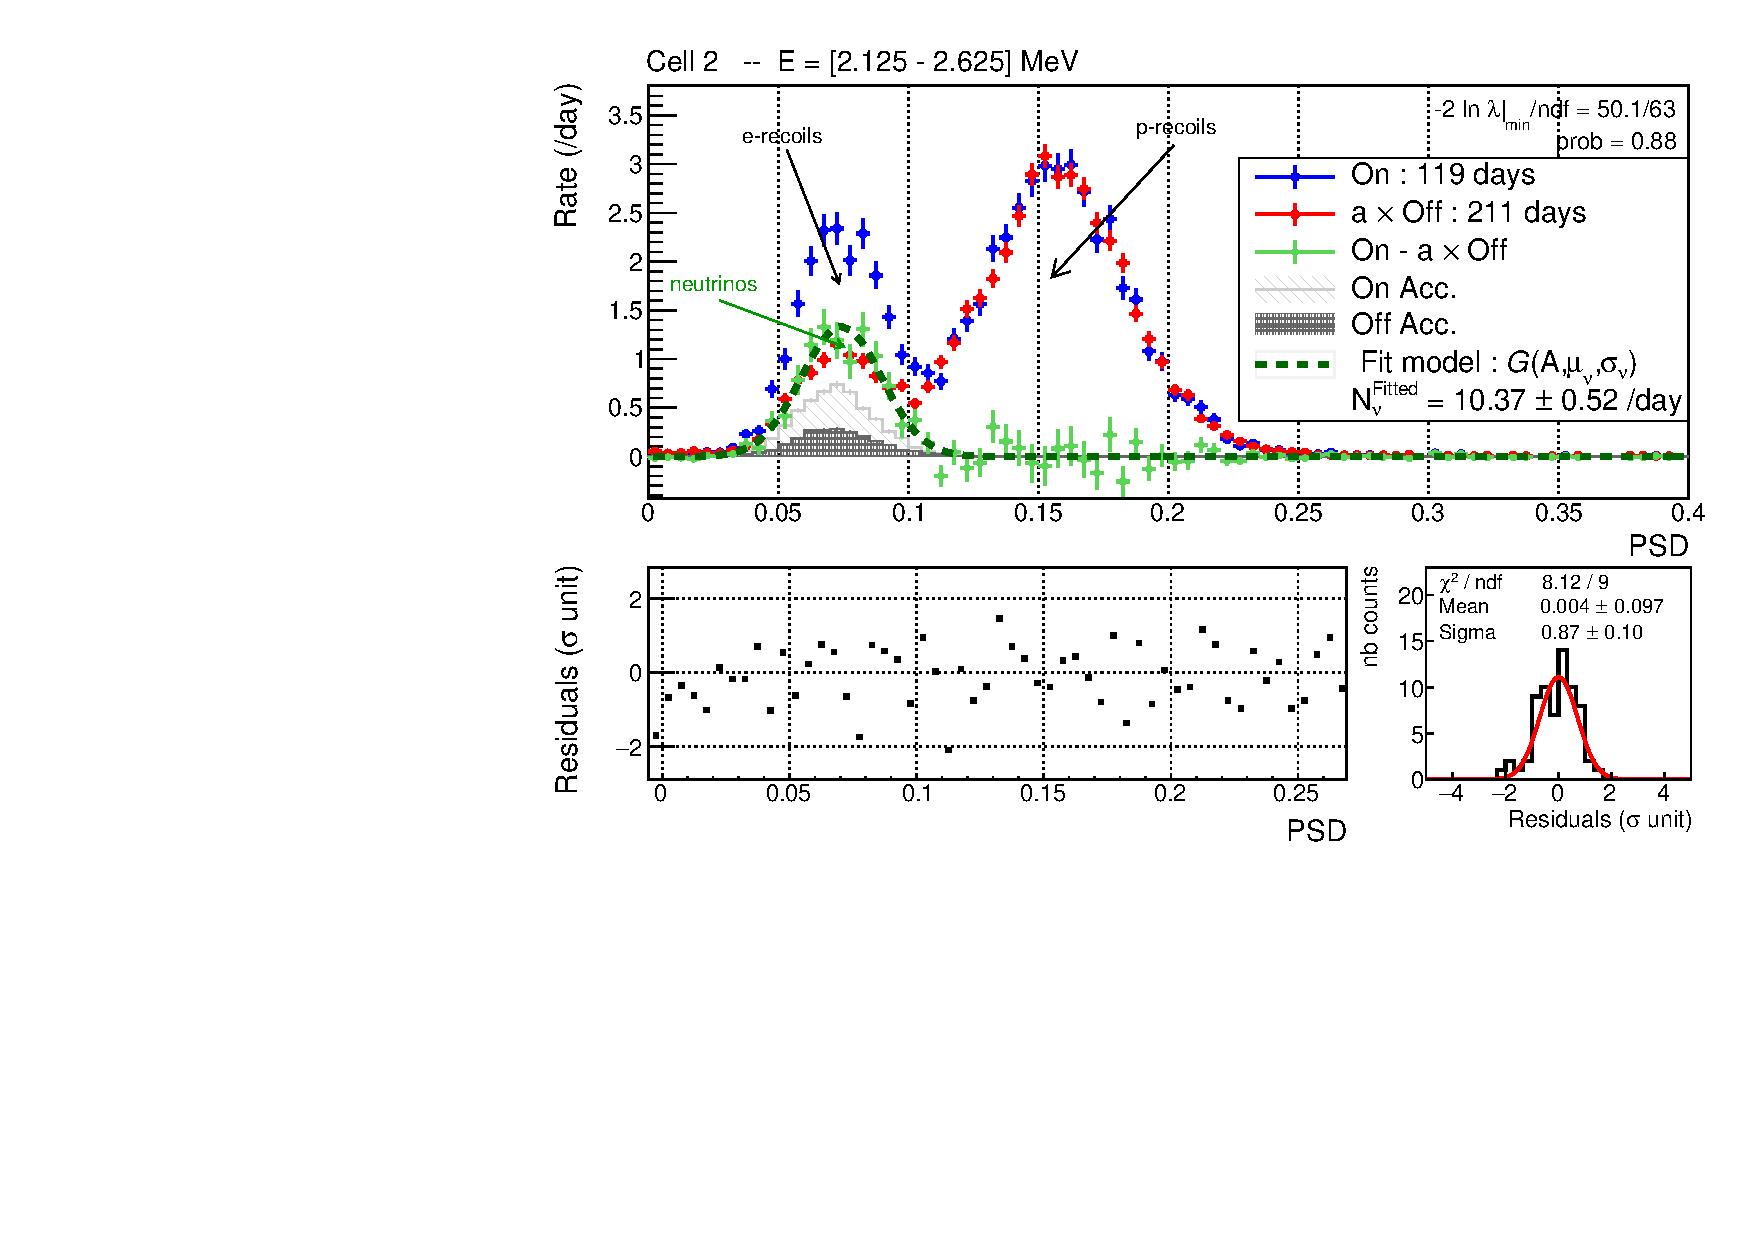
\includegraphics[width=0.9\textwidth]{images/NuExtractionResiduals_Cell2_Ebin2125_P2.pdf}
\caption[Exemple d'extraction du taux de candidats neutrinos par soustraction directe du bruit de fond]{Exemple d'extraction du taux de candidats neutrinos dans la cellule 2 et bin en énergie centrée sur $\SI{2.325}{MeV}$, par soustraction directe du bruit de fond. Les données OFF sont en rouge et les données ON sont en bleu. L'histogramme en vert représente la soustraction effectuée par le $\chi^2$. L'intégrale du modèle neutrino (vert foncé en pointillé) donne le taux de comptage associé à la cellule et au bin en énergie. (source : \cite{docdb966})}
\label{fig:NuExtractionResiduals_Cell2_Ebin2125_P2.pdf}
\end{figure}

}

En pratique un logarithme de vraisemblance est employé pour tenir compte des bins de PSD avec peu de statistique. Ce dernier est écrit sous la forme suivante:

\begin{equation}
    - ln(\mathcal{L}) = - ln(\mathcal{L}(\color{blue}ON_i\color{black})) - ln(\mathcal{L}(\color{red}OFF_i\color{black})) - ln(\mathcal{L}(\color{darkgray}ON_i^\textrm{acc}\color{black} )) - ln(\mathcal{L}(\color{darkgray}OFF_i^\textrm{acc} \color{black})).
\end{equation}

\bigbreak

Comme précédemment, le taux de comptage $\color{black!30!green}A_\nu\color{black}$ est extrait pour chaque bin en énergie et chaque cellule. Un exemple d'ajustement est présenté sur la figure \ref{fig:NuExtractionResiduals_Cell2_Ebin2125_P2.pdf}.\\

L'hypothèse nécessaire pour appliquer cette méthode concerne la stabilité de la forme du bruit de fond. En guise de test de robustesse, les données OFF ont été séparées en deux groupes de dates : haute pression (OFF1) et basse pression (OFF2). Si les formes des distributions en PSD ne changent pas malgré les variations de pression, alors les deux jeux de données peuvent être superposés en appliquant un facteur d'échelle $a$ : $OFF1_i = a \times OFF2_i$ où $i$ représente le bin de PSD. Ce paramètre a été laissé libre pour minimiser le $\chi^2$ entre les deux distributions:

\begin{equation}
    \chi^2 = \sum_i^{PSD} \frac{\left(OFF1_i - a \times OFF2_i\right)^2}{\sigma^2_i(OFF1) + \sigma^2_i(OFF2)}
\end{equation}

\afterpage{

% PSDfigures_pressure_Target.pdf
\begin{figure}[h!]
\centering
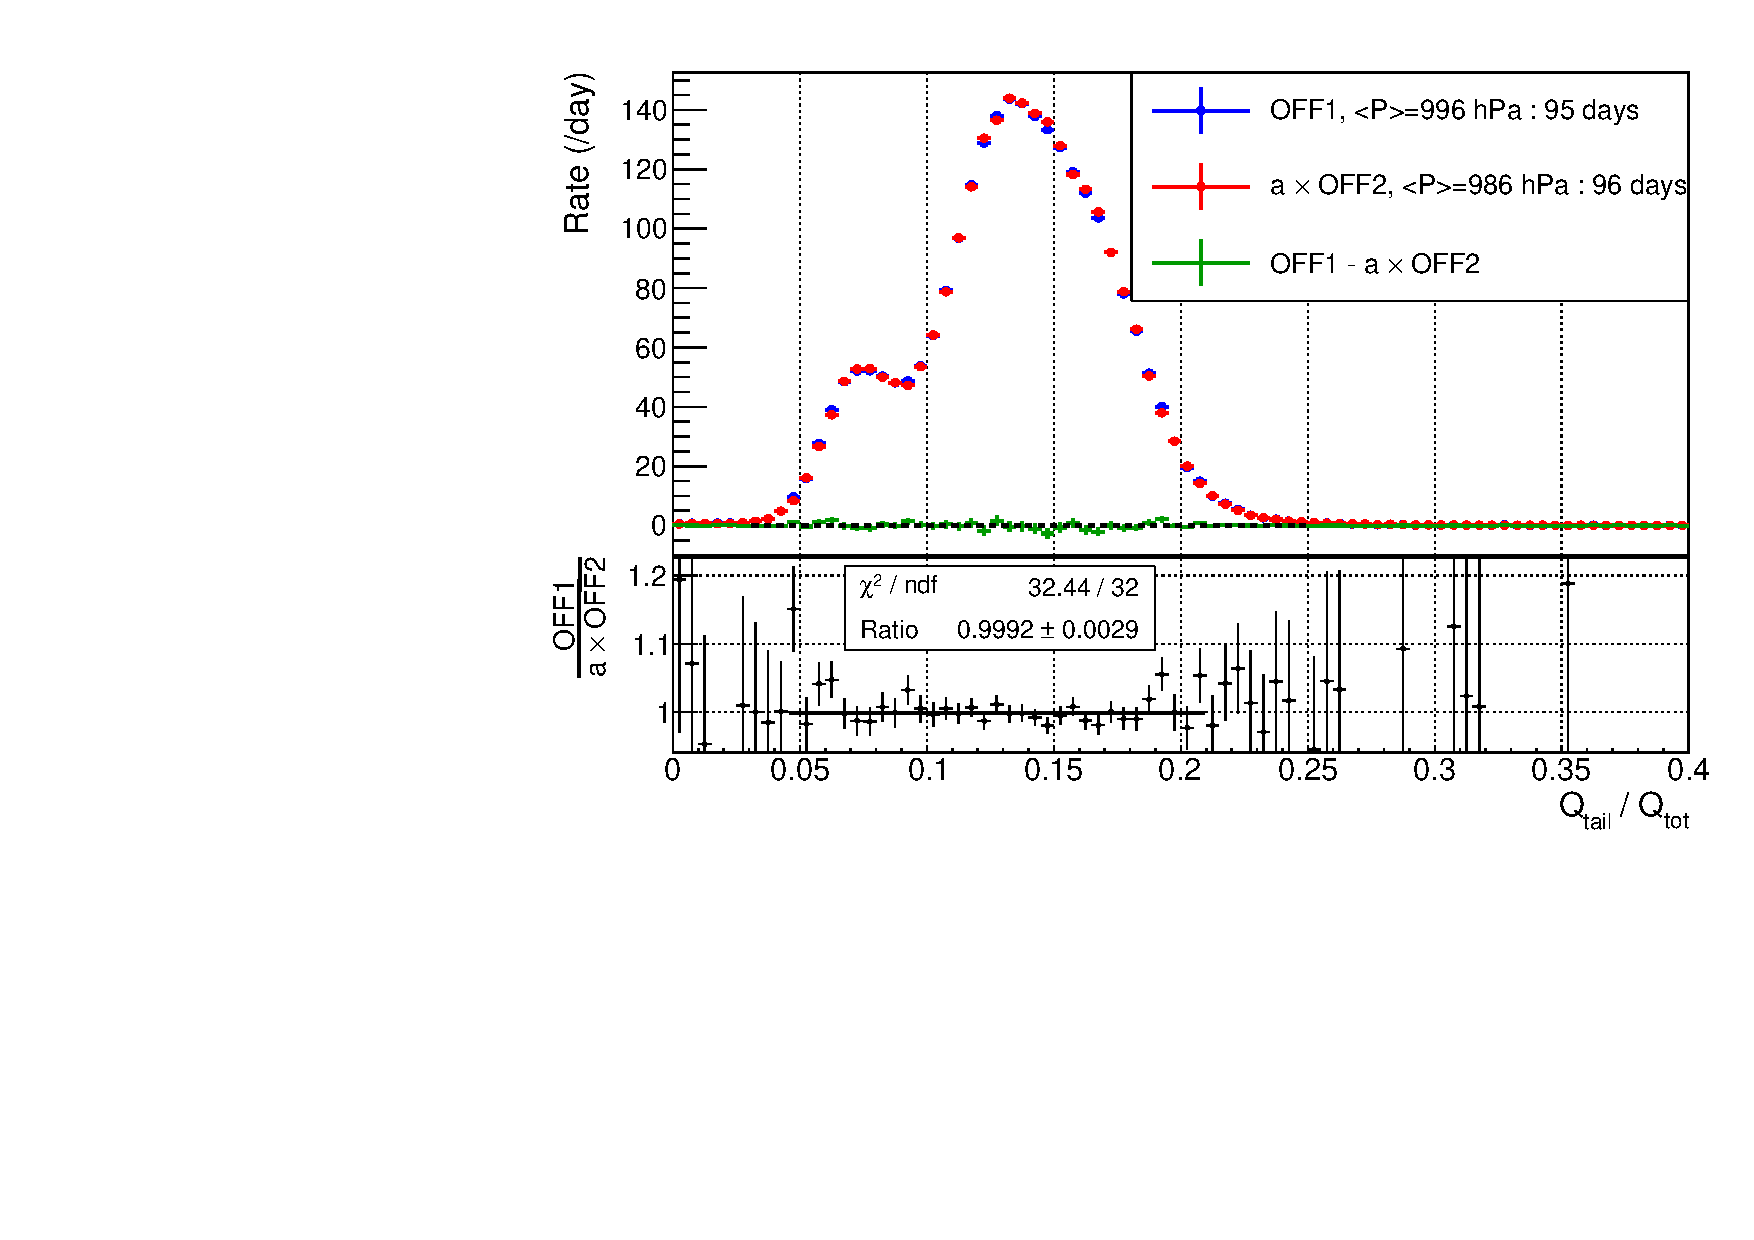
\includegraphics[width=0.8\textwidth]{images/PSDfigures_pressure_Target.pdf}
\caption[Test de stabilité de la forme en PSD du bruit de fond]{Test de stabilité de la forme en PSD du bruit de fond. Les données OFF ont été découpées en deux groupes : haute pression et basse pression. En appliquant un facteur d'échelle sur les données basse pression, les deux distributions montrent un très bon accord. (source : \cite{docdb849})}
\label{fig:PSDfigures_pressure_Target.pdf}
\end{figure}

\begin{figure}[h!]
\centering
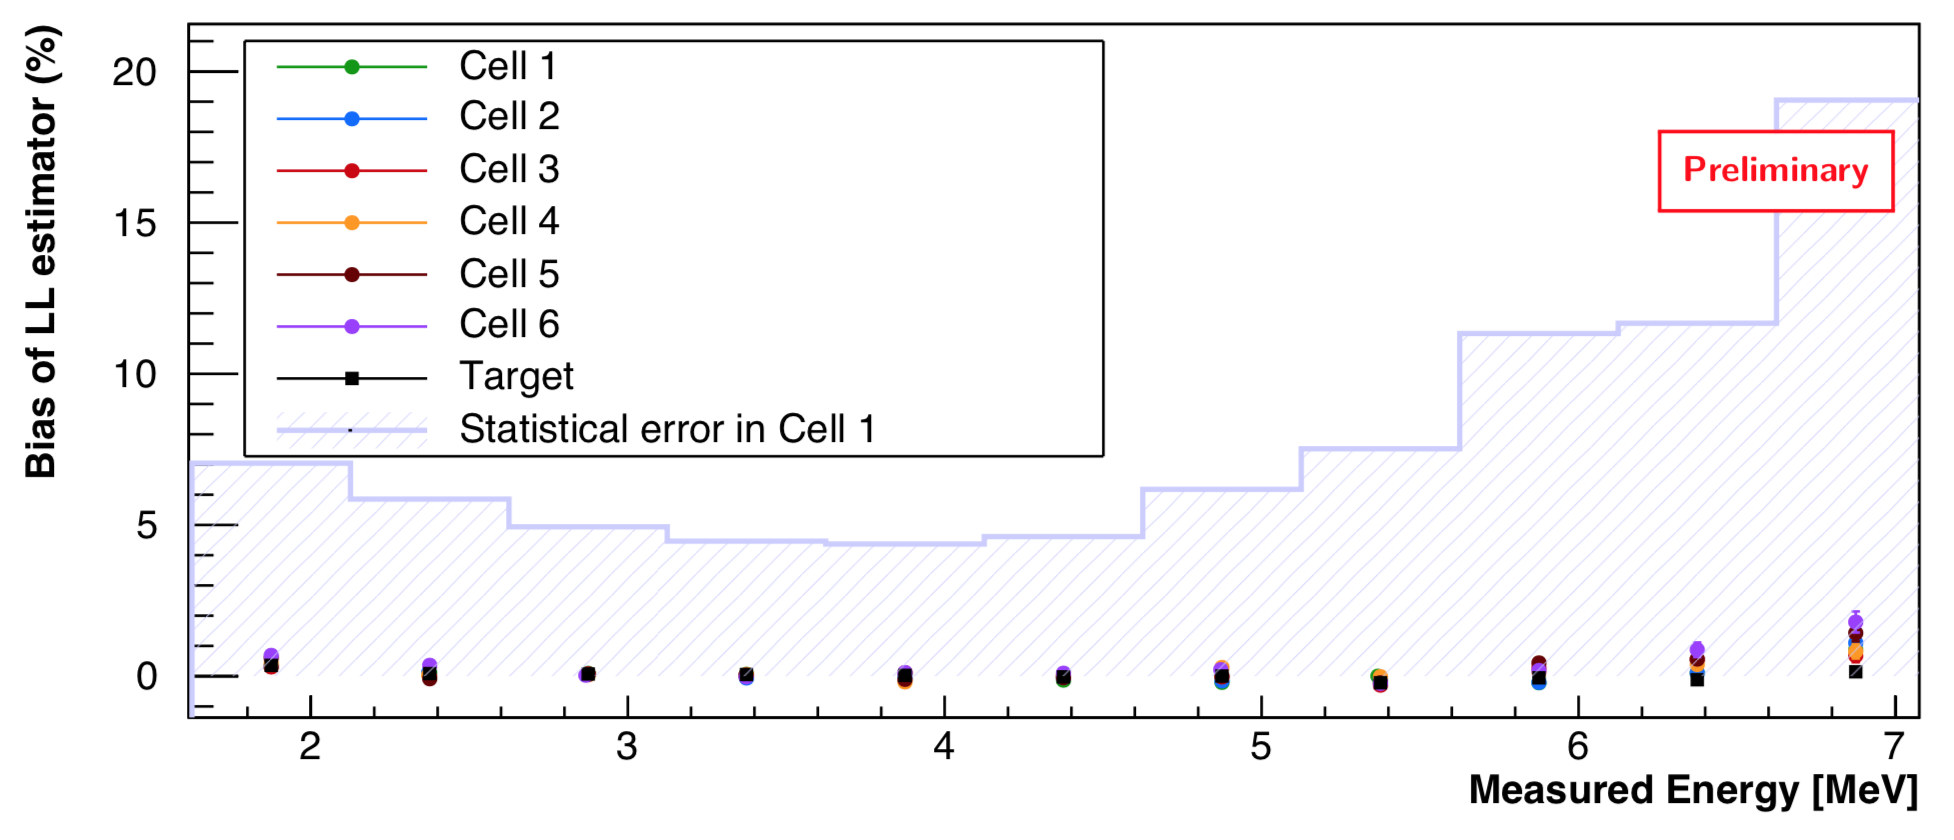
\includegraphics[width=0.8\textwidth]{images/biaisLL_vs_stat.png}
\caption[Biais de l'estimateur vraisemblance sur la mesure du taux de neutrino dans chaque bin en énergie]{Biais de l'estimateur vraisemblance sur la mesure du taux de neutrino dans chaque bin en énergie. L'erreur statistique de la cellule 1 est représentée par la zone hachurée. (source : \cite{docdb849})}
\label{fig:biaisLL_vs_stat.png}
\end{figure}

}

\bigbreak

où $\sigma^2_i(OFF1)$ et $\sigma^2_i(OFF2)$ représentent l'erreur statistique associée à OFF1 et OFF2 respectivement. Le résultat de l'ajustement de $a$ est présenté sur la figure \ref{fig:PSDfigures_pressure_Target.pdf} avec les résidus dans chaque bin en PSD. Le $\chi^2$ minimisé (avec $a$ ajusté) a une valeur de 32,44 pour 32 degrés de liberté, qui s'interprète avec une \textit{p-value} de $\sim 45\%$, témoigne du très bon accord en forme des deux distributions. De plus, le paramètre $a$ peut être prédit d'après les coefficients de corrélation entre la pression et le taux de bruit de fond (noté $a_{corr}$). Là aussi, la valeur estimée est en accord avec celle ajustée : $a_{fit} = (93,3 \pm 0,26) \%$ et $a_{corr} = (93,8 \pm 0,3) \%$.\\

Par ailleurs, le niveau d'eau de la piscine de stockage située juste au-dessus de \textsc{Stereo} affecte le flux de bruit de fond. Comme pour les études avec la pression, les données sont séparées en deux groupes : lorsque le niveau est bas (\SI{7}{m}) et quand le niveau est haut (\SI{15}{m}). Ici aussi le résultat de l'ajustement est très satisfaisant : $\chi^2/\textrm{ndf} = 27/32$.\\

Enfin il est important de noter qu'à très basse statistique la maximisation de la vraisemblance est un estimateur dont le biais croit comme l'inverse du taux de comptage neutrino \cite{CIS-6239} :

\begin{equation}
    \textrm{bias}(A_\nu) \propto \frac{\kappa}{A_\nu} + \mathcal{O}\left(\frac{1}{A_\nu^2} \right).
\end{equation}

où $\kappa$ est une constante donc l'expression dépend la vraisemblance. Ces biais sont estimés à l'aide de \og pseudo-expériences \fg{} qui consistent à générer des distributions de PSD (selon la taille des erreurs statistiques) et d'extraire le taux de neutrinos qui a été injecté. La méthode est détaillée dans le Chapitre \ref{chap:chapitre_stat}.  En choisissant des bins en énergie de largeur $\SI{500}{keV}$, les biais ne dépassent pas 2 \% et restent très faibles comparés à l'erreur statistique comme le montre la figure \ref{fig:biaisLL_vs_stat.png}. Ces biais sont finalement corrigés après avoir extrait les spectres neutrino.

\bigbreak

\subsubsection*{Vérification croisée des deux méthodes}

Les résultats obtenus par les deux méthodes d'extraction des spectres neutrinos ont été comparés pour identifier d'éventuelles erreurs. D'abord, puisque les analyses exploitent des algorithmes de recherche de paires corrélées en temps différents, le calcul du temps effectif est achevé par des procédures indépendantes. Néanmoins, les temps d'acquisition en ON et en OFF pour la phase 2 mesurés par les deux méthodes sont en accord à $\pm 0.1 \%$ \cite{docdb936}. Aussi, les taux de comptage neutrino total sont en accord à $\pm 1.6\sigma$ :

\begin{align}
    A_\nu^{LPSC} = 365.7 \pm 3.2 \SI{}{\nu/day}\\
    A_\nu^{Saclay} = 370.0 \pm 3.3 \SI{}{\nu/day}
\end{align}

\bigbreak

où $A_\nu^{LPSC}$ est le taux de neutrino mesuré par la méthode de soustraction directe du bruit fond (mené par l'équipe de Grenoble au LPSC) et $A_\nu^{Saclay}$ celui obtenu par la méthode de modélisation gaussienne des composantes PSD (effectué au CEA Saclay). La différence peut être due au fait que la méthode de Saclay ne corrige pas encore des biais de l'estimateur du maximum de vraisemblance. Au moment de l'écriture de ce manuscrit, des études sont en cours pour prendre en compte cet effet.\\

\bigbreak

% TODO FM : Conclusion ch5 (et ch4)


%\begin{itemize}
%    \item Coupure PSD et contrôle de l'efficacité
%    \item Présentation méthode Aurélie/Vladimir
%    \item Méthode Laura pour phase2
%    \item tests de stabilité
%\end{itemize}

%\subsection{Tests de robustesse}
%
%\begin{itemize}
%    \item Mesures de l'évolution de la PSD
%    \item Convolution des figures de PSD
%    \item Biais sur l'extraction des rates
%\end{itemize}
%
%\subsection{Comparaison signal et bruit de fond résiduel}
%
%\begin{itemize}
%    \item Figure comparaison spectres bruit de fond / neutrino
%    \item identification des bruits de fond résiduels
%    \item coupures next-gen et gain potentiel sur la précision
%\end{itemize}
%
%\section{Bruits de fond résiduels et optimisation des coupures}
%
% Les bruits de fond susceptibles d'imiter la signature Prompt-Retardé sont classés en deux natures: accidentels ou corrélés. En effet, les procédures de soustraction de ces types diffèrent et elles ont un impact différent sur les erreurs statistiques attribué au signal neutrino. Dès lors, il convient de séparer chaque composante dans l'une de ces deux catégories.
%
%\bigbreak
%
%\subsection{Bruits de fond non corrélés en temps}
%
%\subsection{Bruits de fond corrélés en temps}
%
%\subsection{Optimisation des coupures}
%
%\begin{itemize}
%    \item Critères d'optimisation ? -> acceptance
%    \item Mesure distorsion spectres neutrinos
%    \item Machine learning ?
%\end{itemize}


%\printbibliography

